\RequirePackage[hyphens]{url}

\documentclass[final,a4j,12pt]{jreport}

% 新しいfontの定義? なんだろうこれ
\newfont {\boldmathl}{cmmib10 scaled\magstep1}

% 命令の定義{命令の名前}[引数の個数]
% https://qiita.com/zr_tex8r/items/5067307890d36c0e4882

% \bmを文章中でも使えるように?
\newcommand{\bm}[1]{\mbox{\boldmathl #1}}

% smashは高さを潰す?よくわからん
\newcommand{\lw}[1]{\smash{\lower2.0ex\hbox{#1}}}

% マルチカラムを使うときに必要(だと思う)
\usepackage{multicol}
\usepackage{multirow}

% 数式系を使うときに必要(だと思う)
\usepackage{amsmath,amssymb}

% これを入れておくと画像等の位置指定をするときに強制的にその場所へ置きたい場合[H]を指定できる
\usepackage{here}

% 数式中でベクトルを太字で表現するときに必要
\usepackage{bm}

% 画像の読み込みに必要
\usepackage[dvipdfmx]{graphicx}

% 各種記号
\usepackage{textcomp}

% 部分的に縦書きをするときに必要
\usepackage{plext}

% 番号付き箇条書き(必要なんだっけ?)
\usepackage{enumerate}

% eps形式でもgraphicxを使うのでは?
\usepackage{epsfig}

% コメントアウト環境を使うために必要(必要性が微妙そう?)
\usepackage{comment}

% 長い表を作るときに必要
\usepackage{longtable}

\usepackage{silence}
% Disable all warnings issued by latex starting with "You have..."
\WarningFilter{latex}{You have requested package}

% Japanese Tate Yoko Gosic Minchoの略らしい
% つまり日本語のゴシック、明朝を縦横で使いたいときのパッケージ?
\usepackage{./stylefile/jtygm}

% 参考文献用? コメントアウトしているのはどういうことだろう
% \usepackage{./stylefile/cite}

% 日本語文字と英字が2:1の幅になるverbatimライクな環境 だそうです
% http://konoyonohana.blog.fc2.com/blog-entry-221.html
% \usepackage{./stylefile/jverb}

% hereってえー、これ上のhereと絶対被ってるでしょ
% \usepackage{./stylefile/here}

% 調べても何も出てこない 何?
% ファイルの中身を見たところ卒論用のスタイルファイルだそうです
\usepackage{./stylefile/bpaper}

% epsファイルを使うものらしい graphicxで良くない? コメントアウトされてるしなぁ
% \usepackage{./stylefile/epsbox}

% ページのヘッダーを作るものっぽい
\usepackage{./stylefile/fancyheadings}

% 表の中で斜線を引くためのもの
% \usepackage{./stylefile/slashbox}

% 並べた図に異なる見出しを付ける
% \usepackage{./stylefile/subfigure}

% 参考文献の管理用? よくわからない
\usepackage[backend=bibtex, style=numeric, sorting=none]{biblatex}

% 文字の後にスペースを入れない,という特別扱いをする文字のリストに"'"を追加する
% よくわからないけどbiblatexを使う場合には入れておいた方が良さそう
% https://oku.edu.mie-u.ac.jp/tex/mod/forum/discuss.php?d=2313
\DeclarePrefChars{'-}

% referenceの参照へのパスだろう
% わざわざディレクトリを分ける意味があるのかはわからないが
\addbibresource{./reference/reference.bib}

% 参考文献出力スタイル
% \bibliographystyle{junsrt}

% 置換マクロらしい
% \genfrac{開き括弧}{閉じ括弧}{分数の横棒の太さ}{数式スタイル}{上}{下}
% これ定義する意味あるのか?
\def\frac#1#2{\genfrac{}{}{}{}{\;#1\;}{\;#2\;}}
\def\dfrac#1#2{\genfrac{}{}{}{0}{\;#1\;}{\;#2\;}}
\def\tfrac#1#2{\genfrac{}{}{}{1}{\;#1\;}{\;#2\;}}
\def\sfrac#1#2{\genfrac{}{}{}{2}{\;#1\;}{\;#2\;}}
\def\ssfrac#1#2{\genfrac{}{}{}{3}{\;#1\;}{\;#2\;}}

% いろいろできる表
\usepackage{tabularx}
% これらは何
\newcolumntype{Y}{>{\centering\arraybackslash}X}
\newcolumntype{Z}{>{\raggedleft\arraybackslash}X}

% URLをそのまま書くとチルダとかが無視されるので\url{http://~~}などと書く
\usepackage{url}
% \renewcommand{\url}{\begingroup \def\UrlLeft{}\def\UrlRight{}\urlstyle{rm}\Url}
\PassOptionsToPackage{hyphens}{url}

% 数式とかで使うのか
\def\so{.\raisebox{1ex}{.}.\quad}
% これ三点のこと? それはamsmathがあれば使えそうだけど
\def\because{\raisebox{1ex}{.}.\raisebox{1ex}{.}\quad}

% 超いらなそう……
\def\Omicron{O}
\def\omicron{o}

% 微分記号ですか dy/dxみたいな
\newcommand{\pdif}[2]{\frac{\partial #1}{\partial #2}}

% 見出し番号の深さを6までに指定
\setcounter{secnumdepth}{6}

% プリアンブルの定義・再定義の開始に用いる
% 特に"@"を含むものについて?
\makeatletter

% subsubsubsectionを定義しているのか
\newcommand{\subsubsubsection}{\@startsection{paragraph}{4}{\z@}
  {1.5\Cvs \@plus.5\Cdp \@minus.2\Cdp}
  {.5\Cvs \@plus.3\Cdp}
  {\reset@font\normalsize\sffamily}
}

% argmaxとargminの定義
\newcommand{\argmax}{\mathop{\rm arg~max}\limits}
\newcommand{\argmin}{\mathop{\rm arg~min}\limits}

% 複数行を枠で囲むため
\usepackage{ascmac}

% pandas.DataFrame.to_latexのため
\usepackage{booktabs}

% for 'subtable' environment
\usepackage{subcaption}

% これはエイリアスっぽい
\def\bs#1{\boldsymbol{#1}}
\def\quot#1{``#1''}
\def\ggn{Google {\it N}-gram}

% ページ上部のマージン
\addtolength{\topmargin}{-15mm}
% ページ左側のマージン
\addtolength{\oddsidemargin}{-15mm}

% ここから文書
\begin{document}
\begin{titlepage}
\thesis
{文脈を考慮した一般単語の感情推定}
{Context-sensitive Emotion Estimation for Japanese Words}
{萩原 将文 教授}
% {杉本 麻樹 教授}
{4}
{学籍番号 61914694}
{長澤 尚武}
\end{titlepage}
\pagenumbering{roman}

% 目次
\contents

\pagenumbering{arabic}

\abstract
自然言語処理の分野において,対話応答システムに関する研究は盛んに行われているが,
ユーザに共感し,寄り添うことのできる対話システムの実現には至っていない.
それを実現するための方法として,ユーザの抱いている感情を推定するといったことがあげられる.

そこで本研究では,ユーザの発話に対してその文脈を考慮しながら,
発話内に含まれる単語の感情情報を推定する手法を提案する.
単語を感情に密接に関わる感性語,それ以外の一般単語にわけ,
感性語との共起性をもとに一般単語の感情情報を推定する手法はすでに存在する.
本手法では,ここへ文脈考慮性を導入するために,事前学習モデルの BERT から得られる分散表現を利用した.

BERT は周辺の単語の影響を加味した単語分散表現を出力することが可能である.
この単語分散表現から 10 種類の感情を扱う感情ベクトルを出力するにあたり,
非常にシンプルなニューラルネットワークを採用し,学習を行った.
学習に用いるテキストデータそのものには感情情報に関するラベルを必要としておらず,
感情表現辞典により取得できる感性語とその周辺の一般単語を自動的に抽出して学習することが可能である.
また,出力可能な語彙は BERT で扱うことのできる語彙と同等であるため,
従来の辞書構築型アプローチに比べて対応可能語彙数は大幅に増加した.

これらの性質を利用することにより,同一単語であってもその単語が出現した文脈に応じて,
取得できる感情情報を変化させることができる.
評価実験により,提案手法による単語感情推定の妥当性・文脈考慮性の向上が確認された.


\chapter{はじめに}
自然言語処理の分野において,対話応答システムの研究は盛んにおこなわれている.
身の回りにあるスマートフォンや各種家電といった,様々な製品に搭載されるなど実用化も進み,
人々の生活へ急速に浸透してきている.
しかし,その応答がユーザに寄り添っているようなシステムの実現については,
研究されているもののいまだ課題が残っている.
ユーザに寄り添った対話応答システムが実現することにより,
雑談や気遣いのある応答を行うことが可能になると考えられる.
人々の生活に対話応答システムがより一層浸透し,
人間とコンピュータの連携がより深く円滑に行われることで,
情報化社会の進行に伴う諸問題の解決がより一層促されることが予想される.

ユーザに寄り添った対話応答システムに関する研究の方向性の一つとして,
ユーザの感情推定を行うというものがあげられる.
高村らの研究\cite{spin_kyokusei}では,単語の感情極性,
すなわち単語がポジティブとネガティブのどちらのニュアンスを持つのかを,
電子のスピンの方向に見立てることで推定する手法を提案している.
しかし,人間が抱く複雑な感情を表現するのに2成分では情報量が少ないといえる.
武内らの研究\cite{takeuchi}では,多数の単語に対する感情表現辞書を作成した.
単語が持つ複数の感情情報を取得しているが,
一つの単語に対して一対一で感情情報が保存されているため,
単語がどのように使われているのかという点に対する考慮がなされていない.
Kajiwaraらの研究\cite{kajiwara-wrime}では,SNSへ投稿されたテキストに対し感情情報のラベルを付与し,
投稿者の性格情報と組み合わせることにより文章に対する感情情報を推定している.
しかし,この研究で生成されたデータセットは43200件ほどであり,
より高精度な文感情推定を行う上で更なる拡充を行うには,多大なコストが発生すると考えられる.

そこで本研究では,ラベルのないテキストデータからでもデータセットが生成可能な,
文脈考慮性をもった単語感情推定手法を提案する.
データセットの生成は,感情表現辞典\cite{kanjou_hyogen_jiten}を用いて
感情と密接にかかわる単語(以下,感性語とよぶ)とその単語の持つ感情情報を取得し,
感性語周辺の一般単語を自動的に収集することによりなされる.
そのため,テキストデータに感情情報に関するラベル付けがなされていなくても,
大量の単語感情推定用データセットを生成可能である.
また,事前学習モデルのBERT\cite{BERT}をテキストデータの特徴量抽出機として利用した.
BERTは周囲に存在する単語を考慮した文脈考慮性のある単語分散表現を出力することができる.
例えば,"bank"という単語は同じスペルで"銀行"と"土手"の異なる意味を持つ.
BERTでは,同じ単語だが用いられている意味が異なる場合に
分散表現を変化させることができる,という性質を利用した.


評価実験では,システムへ入力する文章を被験者に作成してもらったうえで,
単語感情推定の妥当性,同一単語を含む文章における感情推定の文脈考慮性を評価した.

以下本論文では,第2章で本研究に関連する研究と知見について述べる.
第3章では提案する文脈を考慮した一般単語感情推定手法について,
第4章では評価実験の内容及び結果について述べる.最後に第5章で結論を述べる.

\chapter{関連する研究と知見}

\section{感情の表現方法}
	感情推定を行う上で,まずは感情の表現方法を定義する必要性がある.
	感情の表現方法の種類として,大きく2種類がある\cite{emotion_analysis_survay}.
	Categorical ModelとDimensional Modelである.

	\subsection{Categorical Model}
		Categorical Modelとは,感情を複数のクラスで表現したものである.
		以下にいくつか例を示す.

		\subsubsection{Ekmanのモデル}
			Ekman\cite{ekman}は怒り,嫌悪,恐れ,喜び,悲しみ,驚きの6つが普遍的な感情であり,生物学的基盤を持つと結論付けている.
			この基準は,異なる文化の人々の表情を読み取ることができるかどうか,である.
			孤立した石器時代の文化で暮らす人々が,他文化の人々の顔の表情を読み取れたかどうかという実験により確認された.

		\subsubsection{Plutchikのモデル}
			Plutchik\cite{plutchik}はEkmanの6感情に加え,信頼と期待を加えた8感情のモデルを提案している.
			本モデルの特徴は喜びと悲しみ,信頼と嫌悪といった形で各感情がそれぞれ対になっている点にある.

		\subsubsection{中村の感情分類}
			中村\cite{kanjou_hyogen_jiten}は,感情表現辞典\cite{kanjou_hyogen_jiten}において,
			言語表現の観点から,感情を「喜, 怒, 哀, 怖, 恥, 好, 厭, 昂, 安, 驚」の10種類に分類している.
			感情表現辞典では,日本の近現代作品の中から様々な感情が入り混じるような微妙な心理を描いた用例を収録している.

	\subsection{Dimensional Model}
		Dimensional Modelとは,感情間の関係を表現するために次元空間を扱うようなモデルのことである.
		感情が連続的であるという仮説の下で表現されたものであり,一般的には2~3次元で表現される.
		主に用いられる次元はvalence(感情価),arousal(覚醒度),dominance(優位性)の3つである.
		valenceは感情が肯定的か否定的かを,arousalは興奮度を,
		dominanceは感情に対する制御度を示している\cite{emotion_model_1}\cite{emotion_model_2}.
		以下にいくつか例を示す.

		\subsubsection{Plutchikの感情の輪}
			Plutchik\cite{plutchik}は,8つの感情をさらに3段階でレベル分けした,
			2次元の感情モデルを提案している.
			次元はvalenceとarousalの2次元である.
			図\ref{fig:plutchik}は,このモデルを図式化したものである.
			\begin{figure}[H]
				\centering
				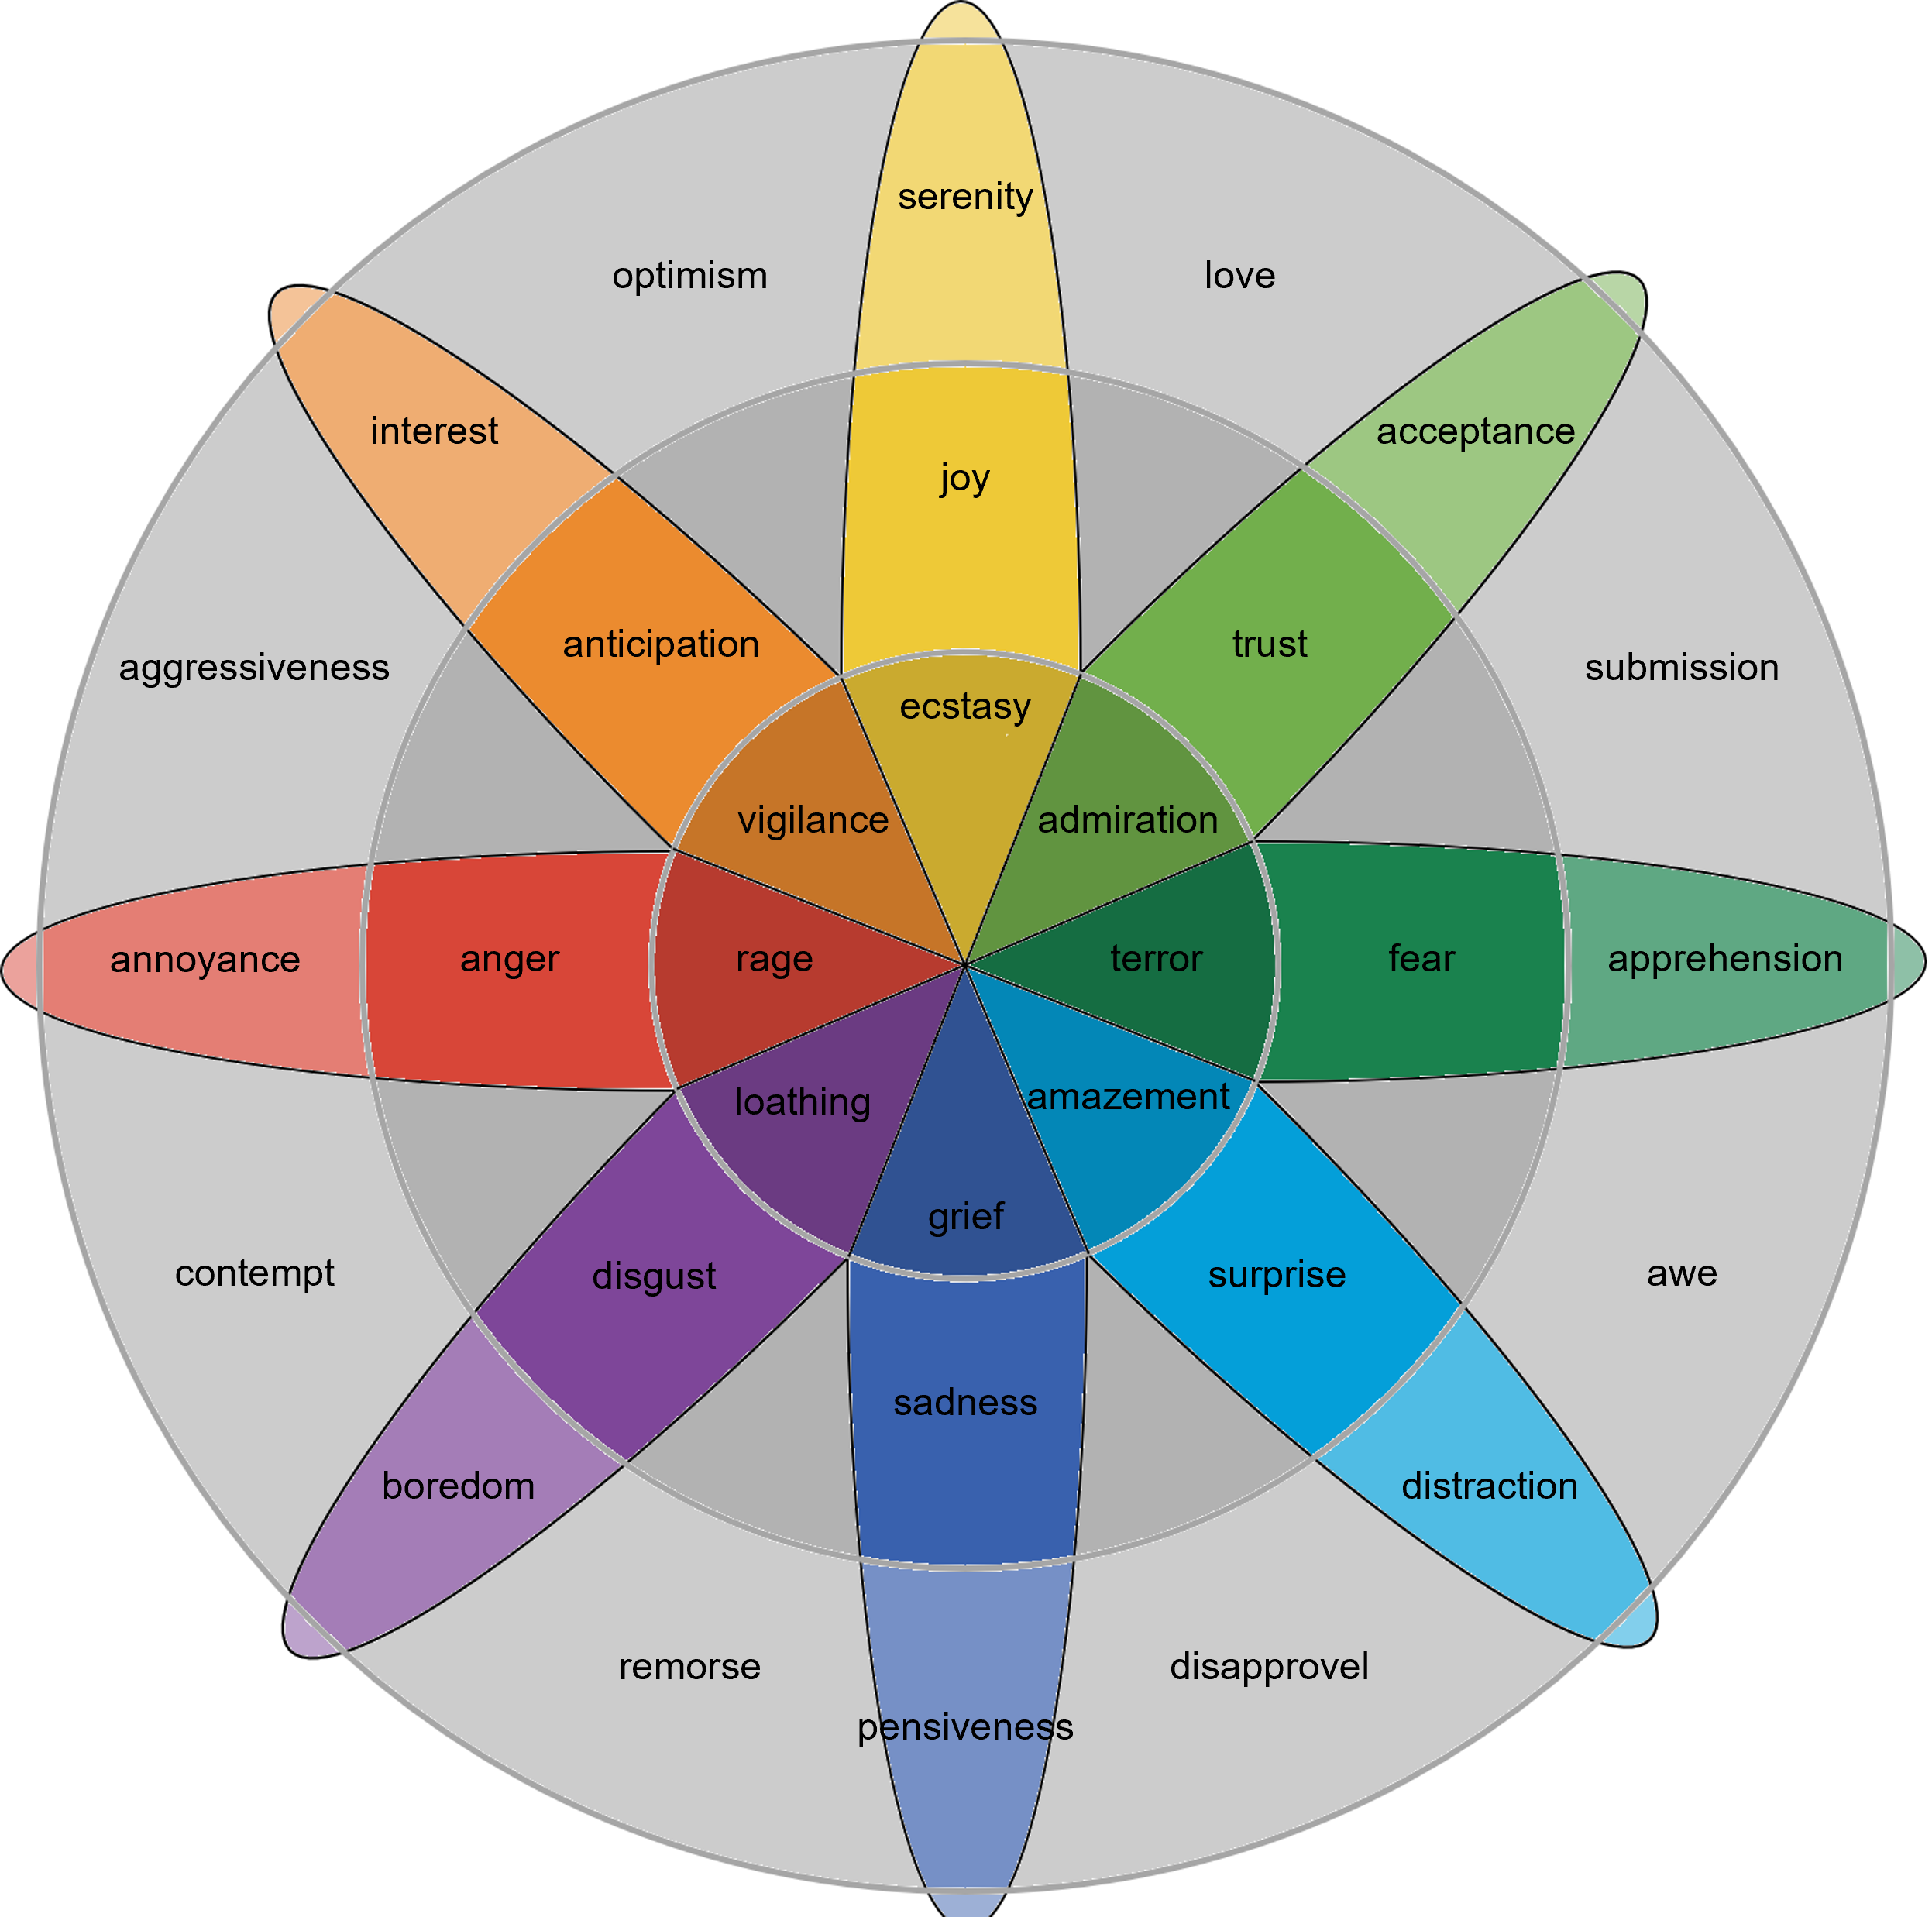
\includegraphics[width=90mm]{./figure/plutchik.png}
				\caption{Plutchikの感情の輪}
				\label{fig:plutchik}
			\end{figure}
			

		\subsubsection{Russellのモデル}
			Russell\cite{russell_2D}は感情をvalence,arousalの2次元で表現する感情モデルを提案した.
			図\ref{fig:russel_2D}は,このモデルを図式化したものである.
			\begin{figure}[H]
				\centering
				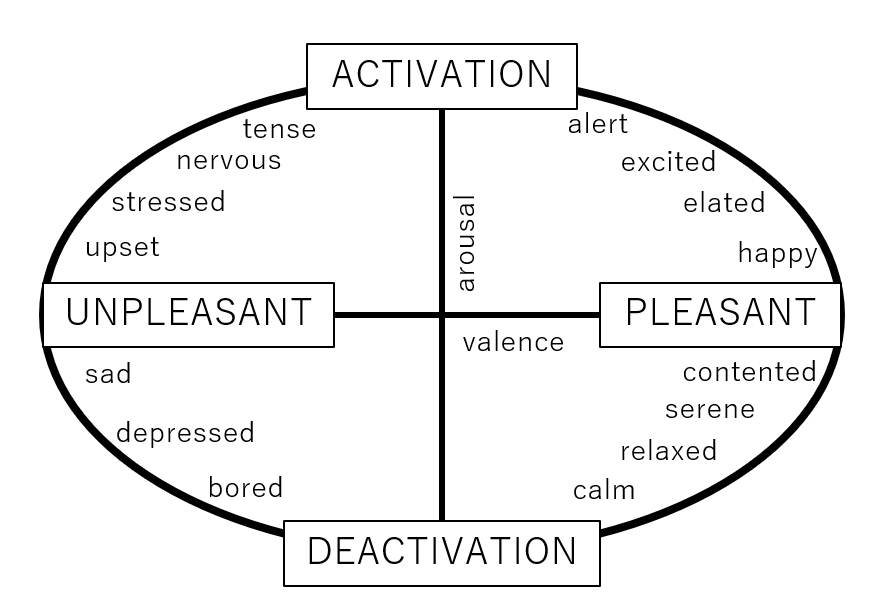
\includegraphics[width=90mm]{./figure/russell.png}
				\caption{Russellのモデル}
				\label{fig:russel_2D}
			\end{figure}

		\subsubsection{Russell, MehrabianのPADモデル}
			RusellとMehrabian\cite{russell_3D}は,Pleasure,Arousal,Dominanceの3次元で表現する感情モデルを提案した.
			PADは各次元の頭文字をとったものである.

\section{コンピュータ上での単語の表現}
	コンピュータは,入力された単語をテキスト情報のまま処理することができない.
	それをかなえるためには,単語のベクトル化が必要となる.

	\subsection{one-hotベクトル}
		one-hotベクトルとは,最も単純な単語のベクトル表現方法である.
		具体的には,語彙内の単語のインデックスに対応した成分だけが1となり,
		その他の成分がすべて0となるようなベクトルである.
		よって,次元数はシステムが扱う語彙数と同数となる.
		図\ref{fig:one-hot-vector}にone-hotベクトルによる表現の例を示す.
		具体的には,サイズが10000語の語彙$V$について,
		語彙内の単語がどのように表現されるのかを表している.
		各単語と対応する語彙内のインデックスが括弧内の数字に対応している.
		各ベクトルは,語彙数と同じ10000次元である.
		\begin{figure}[H]
			\centering
			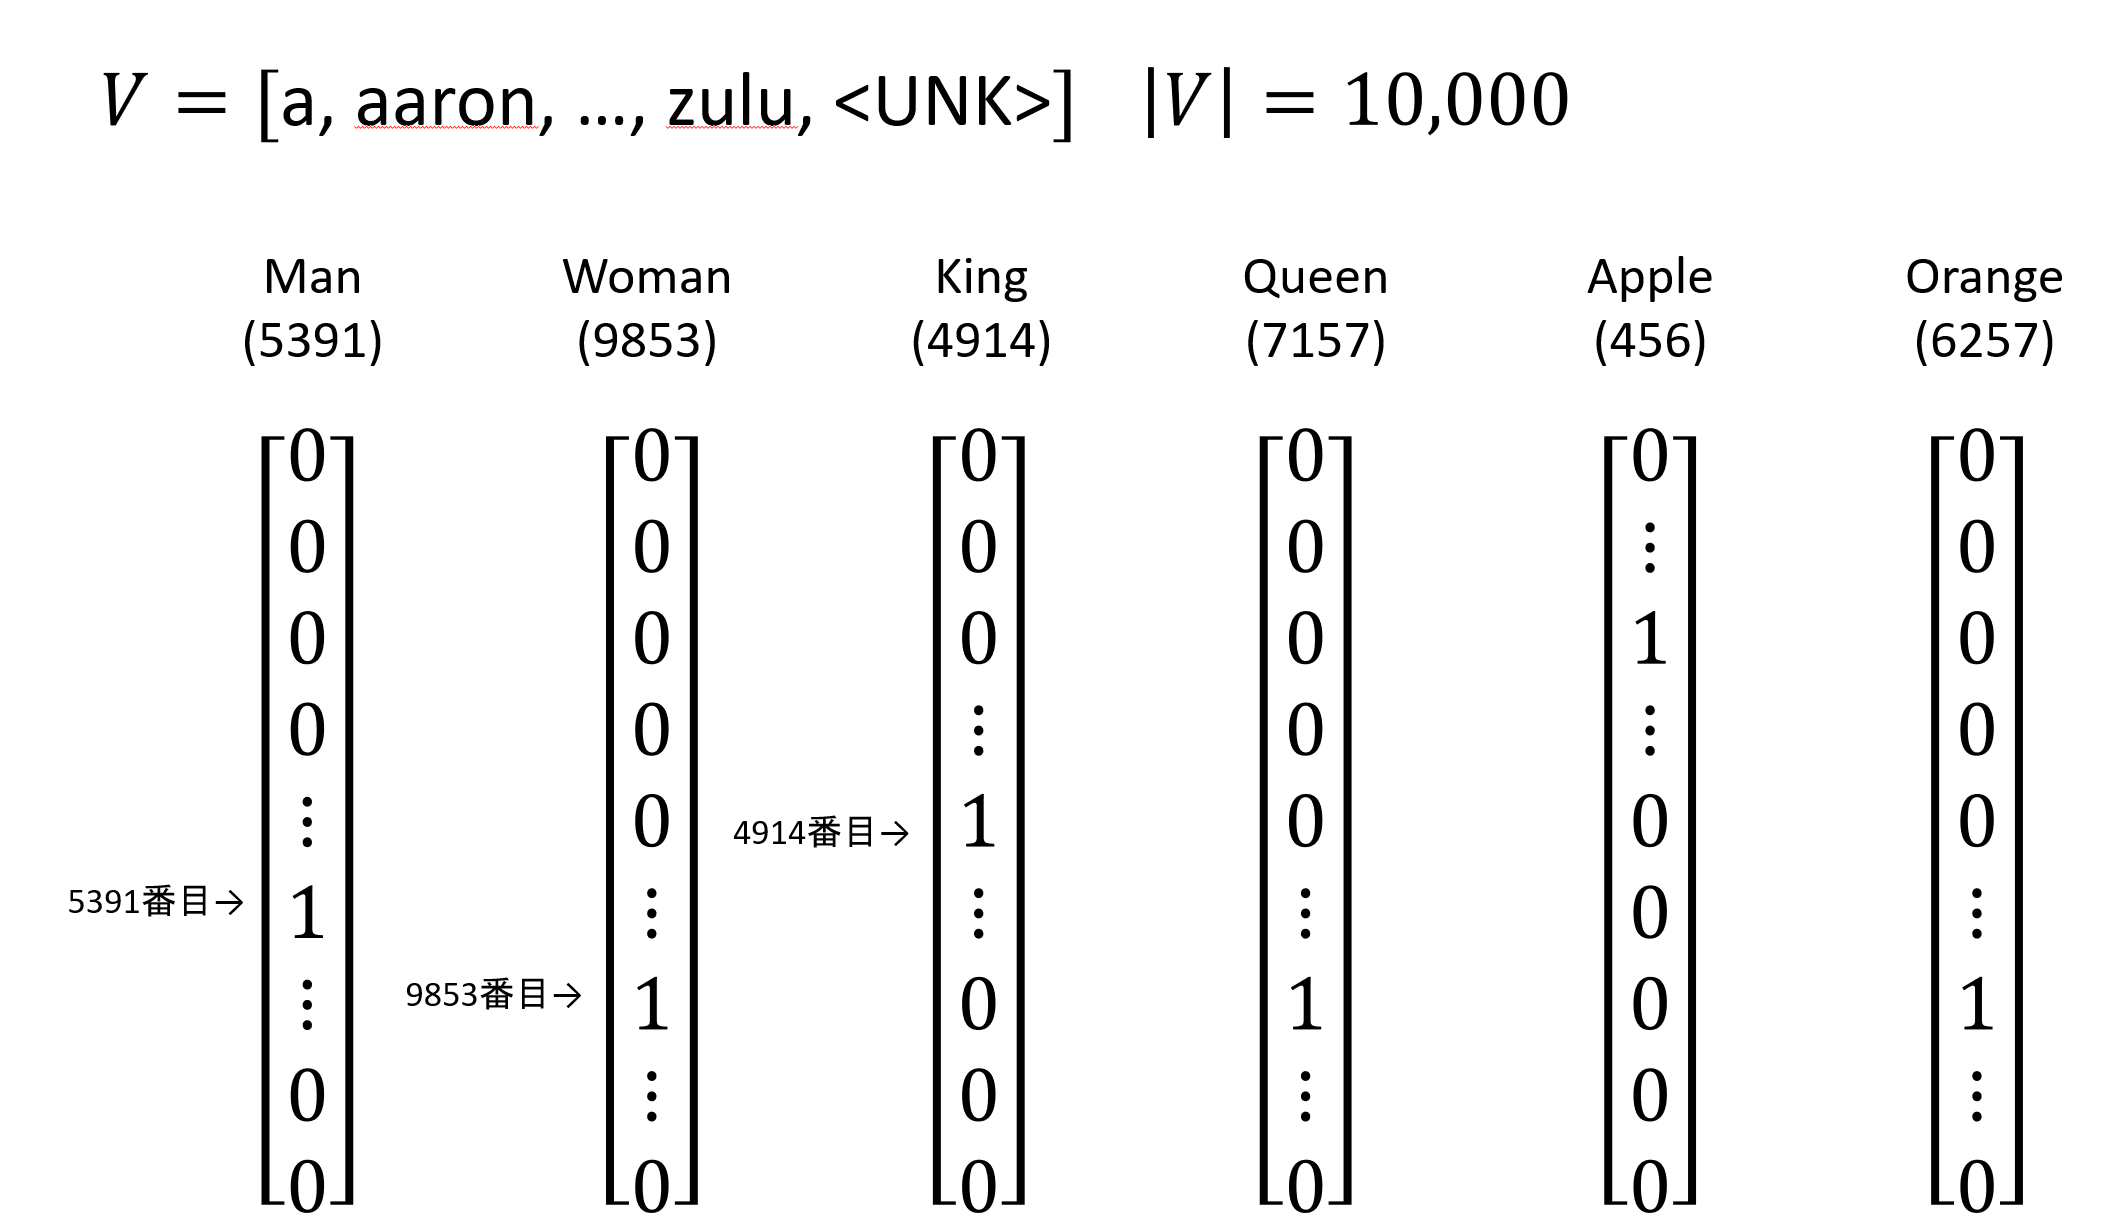
\includegraphics[width=\linewidth]{./figure/one-hot-vector.png}
			\caption{one-hotベクトルの例}
			\label{fig:one-hot-vector}
		\end{figure}

		one-hotベクトルによる単語ベクトルの表現を行う上でのの問題点として,
		システムの扱う語彙数が増えることにより,単語ベクトルの次元数が同量増えてしまうことが挙げられる.
		また,このような非常に次元の高いベクトルであるにもかかわらず,
		ベクトル内の1成分だけが1で他の成分はすべて0となる.
		よって,単語ベクトルが非常に疎なベクトルとなってしまうため,
		消費するリソースのわりに得られる情報量が少ないということも挙げられる

	\subsection{単語分散表現}
		単語分散表現とは,単語をベクトル空間上の一つの点として捉えるような表現方法のことである.
		単語分散表現は各要素が実数値を持つ,密なベクトルとなっていて,
		システムの語彙数よりも低い次元数のベクトルで表現可能である.
		単語のベクトル同士の計算と単語間の意味関係が対応するのが特徴であり,
		このことからもベクトルの各要素が単語の特徴を表していると考えられている.
		図\ref{fig:word2vec}は,単語分散表現の特徴であるベクトル間の計算と
		意味関係の対応を単純化して示したものである.
		
		\begin{figure}[H]
			\centering
			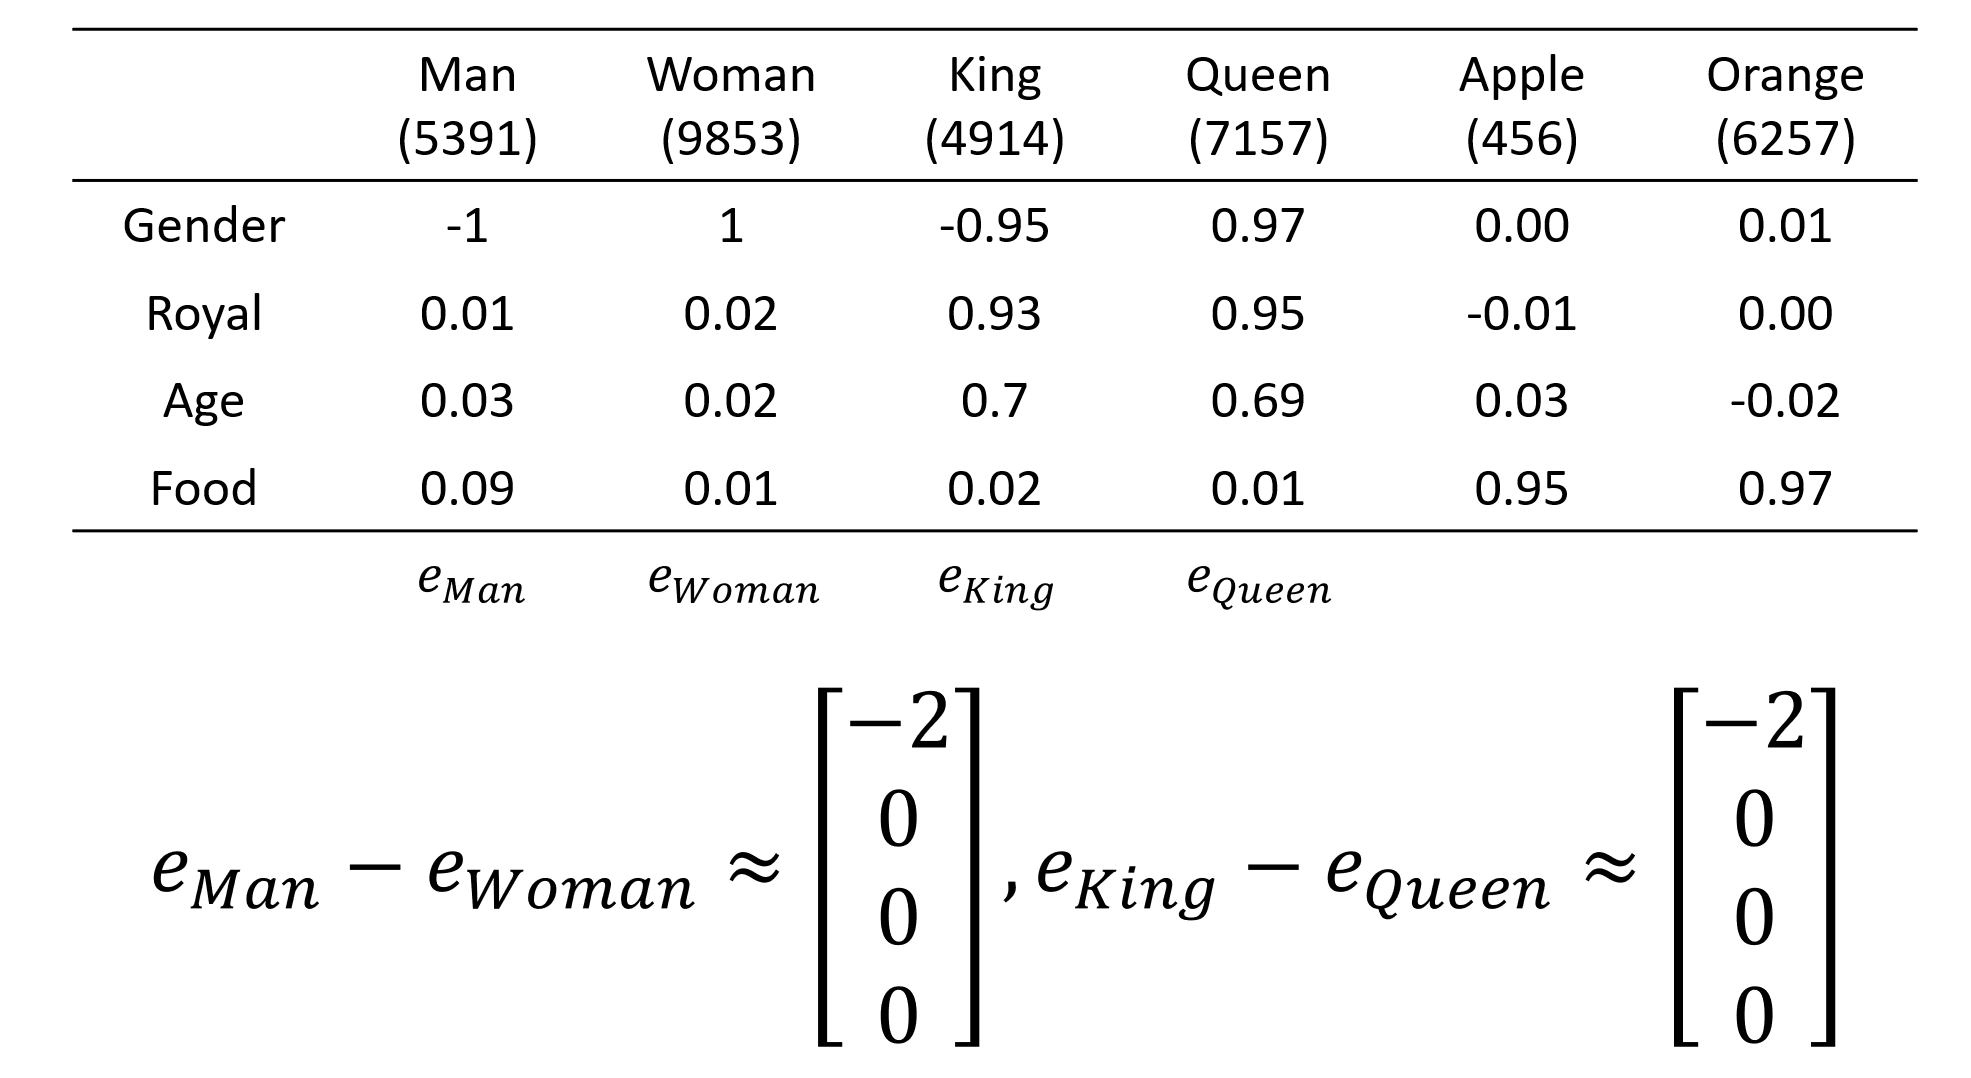
\includegraphics[width=\linewidth]{./figure/word2vec.png}
			\caption{ベクトル同士の計算による単語間の意味関係の取得}
			\label{fig:word2vec}
		\end{figure}

		各成分が特定の意味を持つような4次元のベクトルとして,各単語を表現している.
		この時,"Man"と"Woman"の違いは各ベクトルの差をとることで,
		"Gender"成分にあるということがわかり,
		同様の関係が"King"と"Queen"の間にも認められることがわかる.
		このように,各単語に対応するベクトルの演算結果が,
		単語間の意味関係と対応することになる.
		
		なお,実際に取得される単語分散表現は,より高次元で複雑なものである.
		各成分が持つ意味について人間が把握することは非常に困難であるが,
		ベクトル間の計算と意味関係が一致する性質を踏まえると,
		何かしらの特徴を各成分が表現していると推測される.
		主要な単語分散表現の手法として,Word2Vec\cite{word2vec}やGloVe\cite{glove}などが挙げられる.

\section{CBOWモデルをもとにした単語感情分析手法}
	武内ら\cite{takeuchi}は,Continuous Bag-of-wordsモデルの発想を感情表現の抽出に活用した.

	\subsection{Continuous Bag-of-Wordsモデル}
	Continuous Bag-of-Wordsモデル\cite{word2vec}(以下,CBOWモデルとよぶ)は,Word2Vecを学習するのに用いられる.
	Word2Vecの学習は分布仮説の下で行われる.
	分布仮説とは単語の持つ意味が周囲の単語により決まる,というものである.
	つまり,周りの単語が中心の単語の意味的な要素を持っていることにもなる.

	CBOWモデルは,周りの単語を入力して中央の単語を予測するという形のモデルである.
	図\ref{fig:CBOW}は,CBOWモデルの概要である.

	\begin{figure}[H]
		\centering
		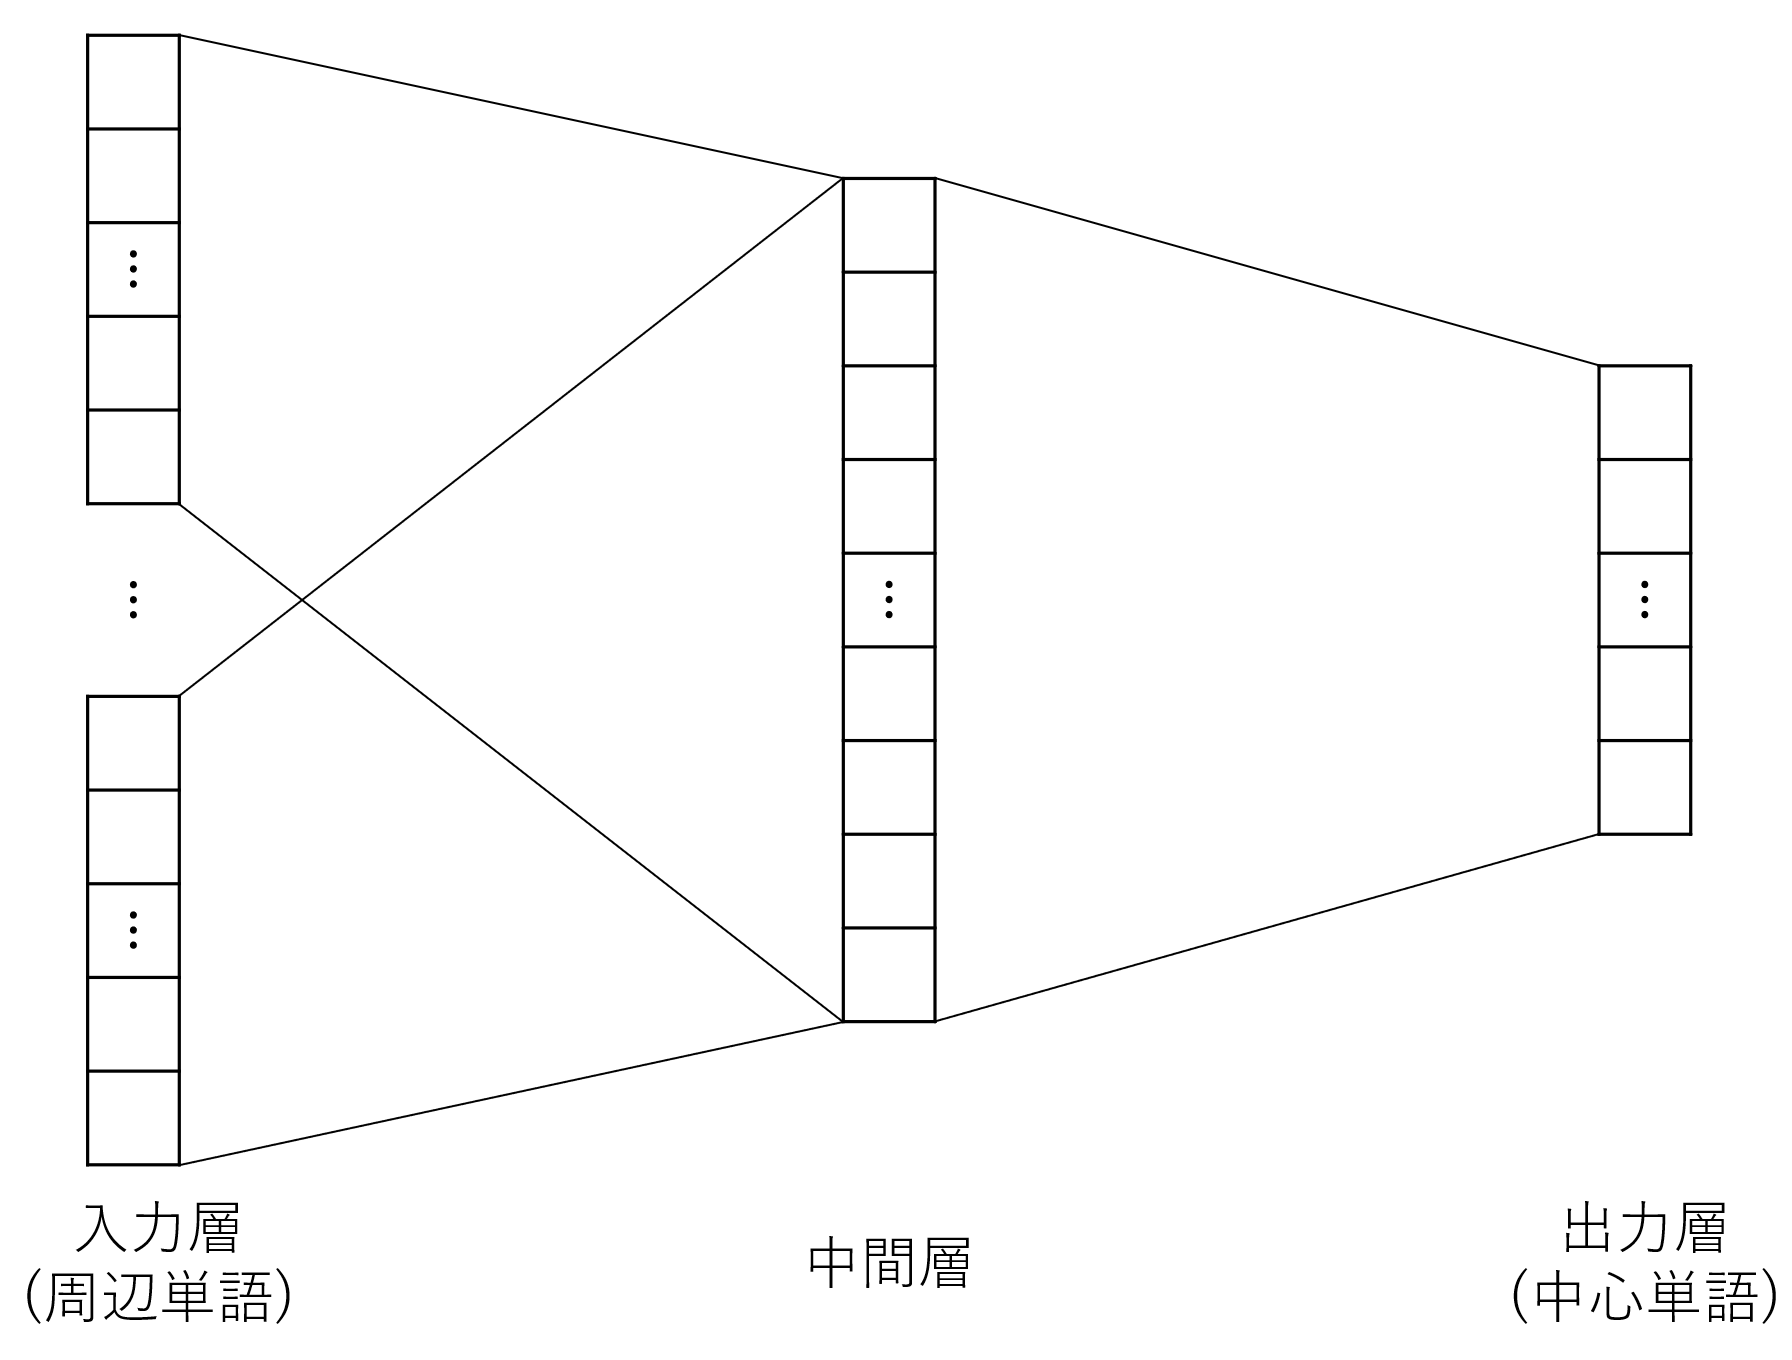
\includegraphics[width=\linewidth]{./figure/CBOW.png}
		\caption{CBOWモデルの概要}
		\label{fig:CBOW}
	\end{figure}

	生成する分散表現の次元数を$d$,語彙数を$V$とすると,
	入力は$V$次元のone-hotベクトル,入力と中間層の間の重みが$(V \times d)$の行列となる.
	中間層は周囲の単語の分散表現の和となり,出力は入力同様に$V$次元のone-hotベクトルで
	中心の単語を出力するという形になる.
	この予測が正しく行えるようにネットワークを学習することで,
	分散表現が単語の意味情報を反映できるようになる.
	

	\subsection{概要}
		\subsubsection{感性語の抽出}
			まず,感情表現辞典\cite{kanjou_hyogen_jiten}から感情と密接にかかわる単語である感性語を取得する.
			この感情表現辞典から得られる感情情報は「喜, 怒, 哀, 怖, 恥, 好, 厭, 昂, 安, 驚」10種類であるため,
			各要素が1つの感情に対応するような10次元のベクトル(以下,感情ベクトルとよぶ)を取得できる.

		\subsubsection{ネットワークの学習}
		テキストデータに対して形態素解析を行い,品詞を絞ったうえで原型に変換する.
		ウィンドウサイズを$W$としたとき,中心の感性語に対し前後$W$個の単語を収集し
		合計$2W+1$個の単語群を一つのデータとする.
		図\ref{fig:takeuchi_dataset}で,周辺単語の収集の様子を示す.
		\begin{figure}[H]
			\centering
			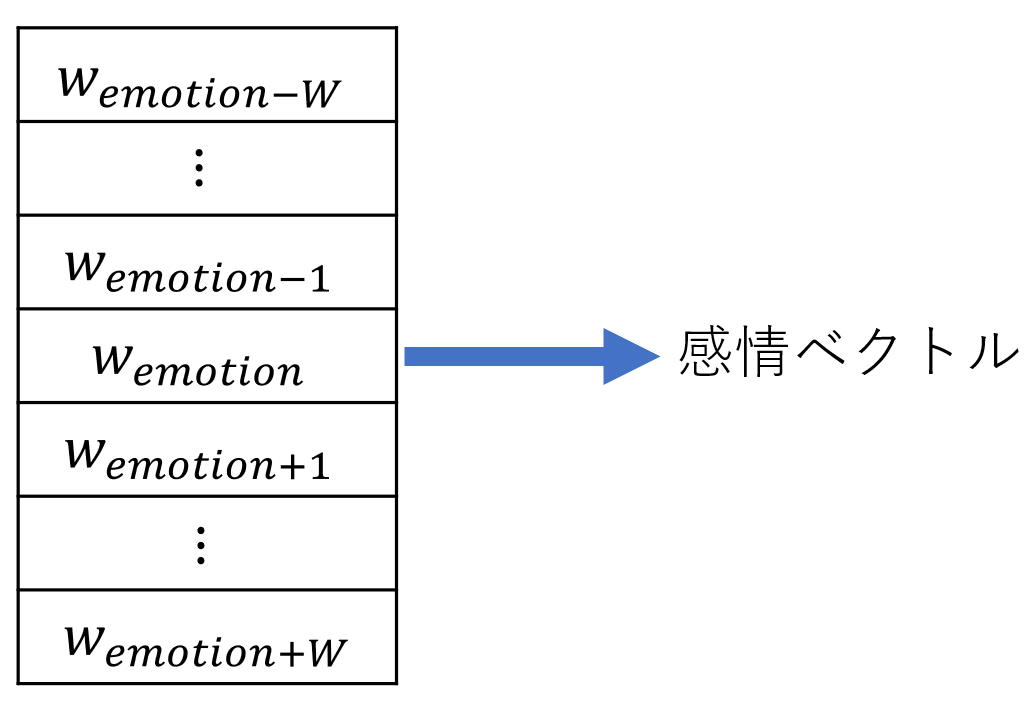
\includegraphics[width=\linewidth]{./figure/takeuchi_dataset.png}
			\caption{データセット生成での単語収集の概要}
			\label{fig:takeuchi_dataset}
		\end{figure}
		入力はそれぞれの単語に対するone-hotベクトルで,
		中間層は感情ベクトルと同じ10次元のベクトルとなる.
		語彙数を$V$としたとき,入力層と中間層の間の重みは,$(V \times 10)$の行列で,
		中間層は入力単語群から変換された10次元のベクトルの和となる.
		この中間層のベクトルをsoftmax層に通したときに,
		中心の感性語が持つ感情ベクトルとの差がなくなるようにしてネットワークを学習する.
		softmax関数は以下の式で示される.
		\begin{equation}
			p_k = \frac{e^{x_k}}{\sum_{i=1}^{10}e^{x_i}}
		\end{equation}
		softmax関数に入力する中間層は10次元で,$x_k$はそのうちの$k$番目の値である.
		softmax関数により,値の総和が1となるような同次元数の出力を得ることができる.
		この時,出力はウィンドウサイズ内の単語を入力した際に推定される感情の確率分布とみなされる.
		以上のような学習により,
		入力層と中間層の間の重みの各行が対応する単語に対する感情ベクトルとなる.

		\subsubsection{出力}
		上述のような学習を行うことにより,各単語に対する10次元の感情ベクトルを取得することができる.
		感情ベクトルの各成分はそれぞれ,「喜, 怒, 哀, 怖, 恥, 好, 厭, 昂, 安, 驚」の感情に対応している.
		これらの感情は,感情表現辞典から得られる情報に対応している.

	\subsection{出力例}
		以下に本手法で得られる出力例を示す.

		\begin{figure}[H]
			\centering
			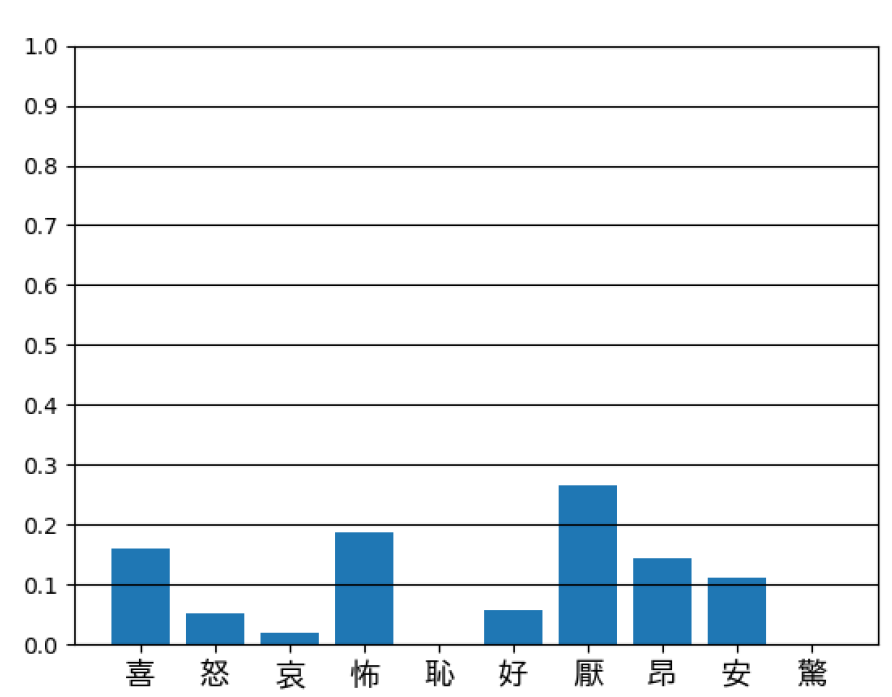
\includegraphics[width=110mm]{./figure/takeuchi_output_toushi.png}
			\caption{本手法で得られる「投資」に対する感情ベクトルの例}
			\label{fig:takeuchi_output_1}
		\end{figure}

		\begin{figure}[H]
			\centering
			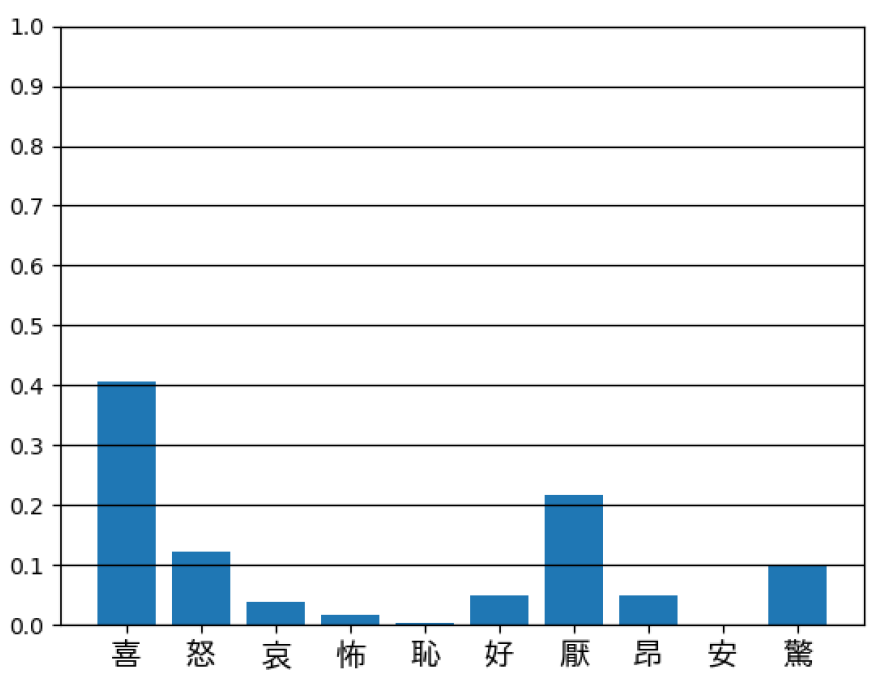
\includegraphics[width=110mm]{./figure/takeuchi_output_seiseki.png}
			\caption{本手法で得られる「成績」に対する感情ベクトルの例}
			\label{fig:takeuchi_output_2}
		\end{figure}

		本手法で得られる感情ベクトルの特徴は,一つの単語に対して,
		想起しうる感情が複数現れることが挙げられる.
		図\ref{fig:takeuchi_output_1}では,「投資」という単語に対する
		感情ベクトルを示している.
		「投資に成功して儲けが出た」,という文脈においては,
		投資に対してポジティブな印象を持っていると考えられる.
		反面,「投資に失敗してしまった」,という文脈においては,
		投資に対してあまり良い印象を持っていないと考えられる.
		また,投資を行ったことがない,という人にとっては
		怖いものとして扱われるケースも想定される.
		これらの,想定しうる「投資」のイメージを
		感情ベクトルがよく反映しているといえる.
		図\ref{fig:takeuchi_output_2}では,「成績」という単語に対する
		感情ベクトルを示している.
		成績も人や試験等の結果によって抱く印象は様々であり,
		出力でも同様の傾向が見られている.

		このように本手法では,
		単語が用いられる文脈によって想起されうる感情が異なってくることを
		感情ベクトルとして表現することができる.
	
	\vskip\baselineskip
	本研究では,一般単語に対して想起しうる感情情報を抽出している.
	しかし,その情報を使って対話システム等に応用することを考えると,
	単語から想起しうる複数の感情が想起されるのは好ましくない.
	単語がどのような文脈で用いられたかを踏まえたうえでの感情推定ができれば,
	後続のタスクへ適切な感情情報を与えることができる.

\section{BERT}
	Bidirectional Encoder Representations from Transformers\cite{BERT}(以下,BERTとよぶ)は,
	2018年にGoogleから発表された事前学習言語モデルである.
	\subsection{特徴}
		BERTは入力として,文章をトークンに分割したものを用い,出力として,各トークンに対応したベクトルを出力する.
		BERT以前の自然言語処理で主流であったRecurrent Neural Network(以下,RNNとよぶ)ベースのモデルと
		同様の入出力形式である.
		RNNベースのモデルでは,長い文章を入力しても最初の方の情報を保持することができない
		という課題があった.
		しかしBERTでは,Transformer Encoder\cite{attention}により
		トークンの処理に他のトークンの情報を直接的に用いることができる.
		これに伴い,各トークンについてより文脈に即した分散表現を出力することができる.
		図\ref{fig:bert}は,BERTの概要を図式化したものである.
		
		\begin{figure}[H]
			\centering
			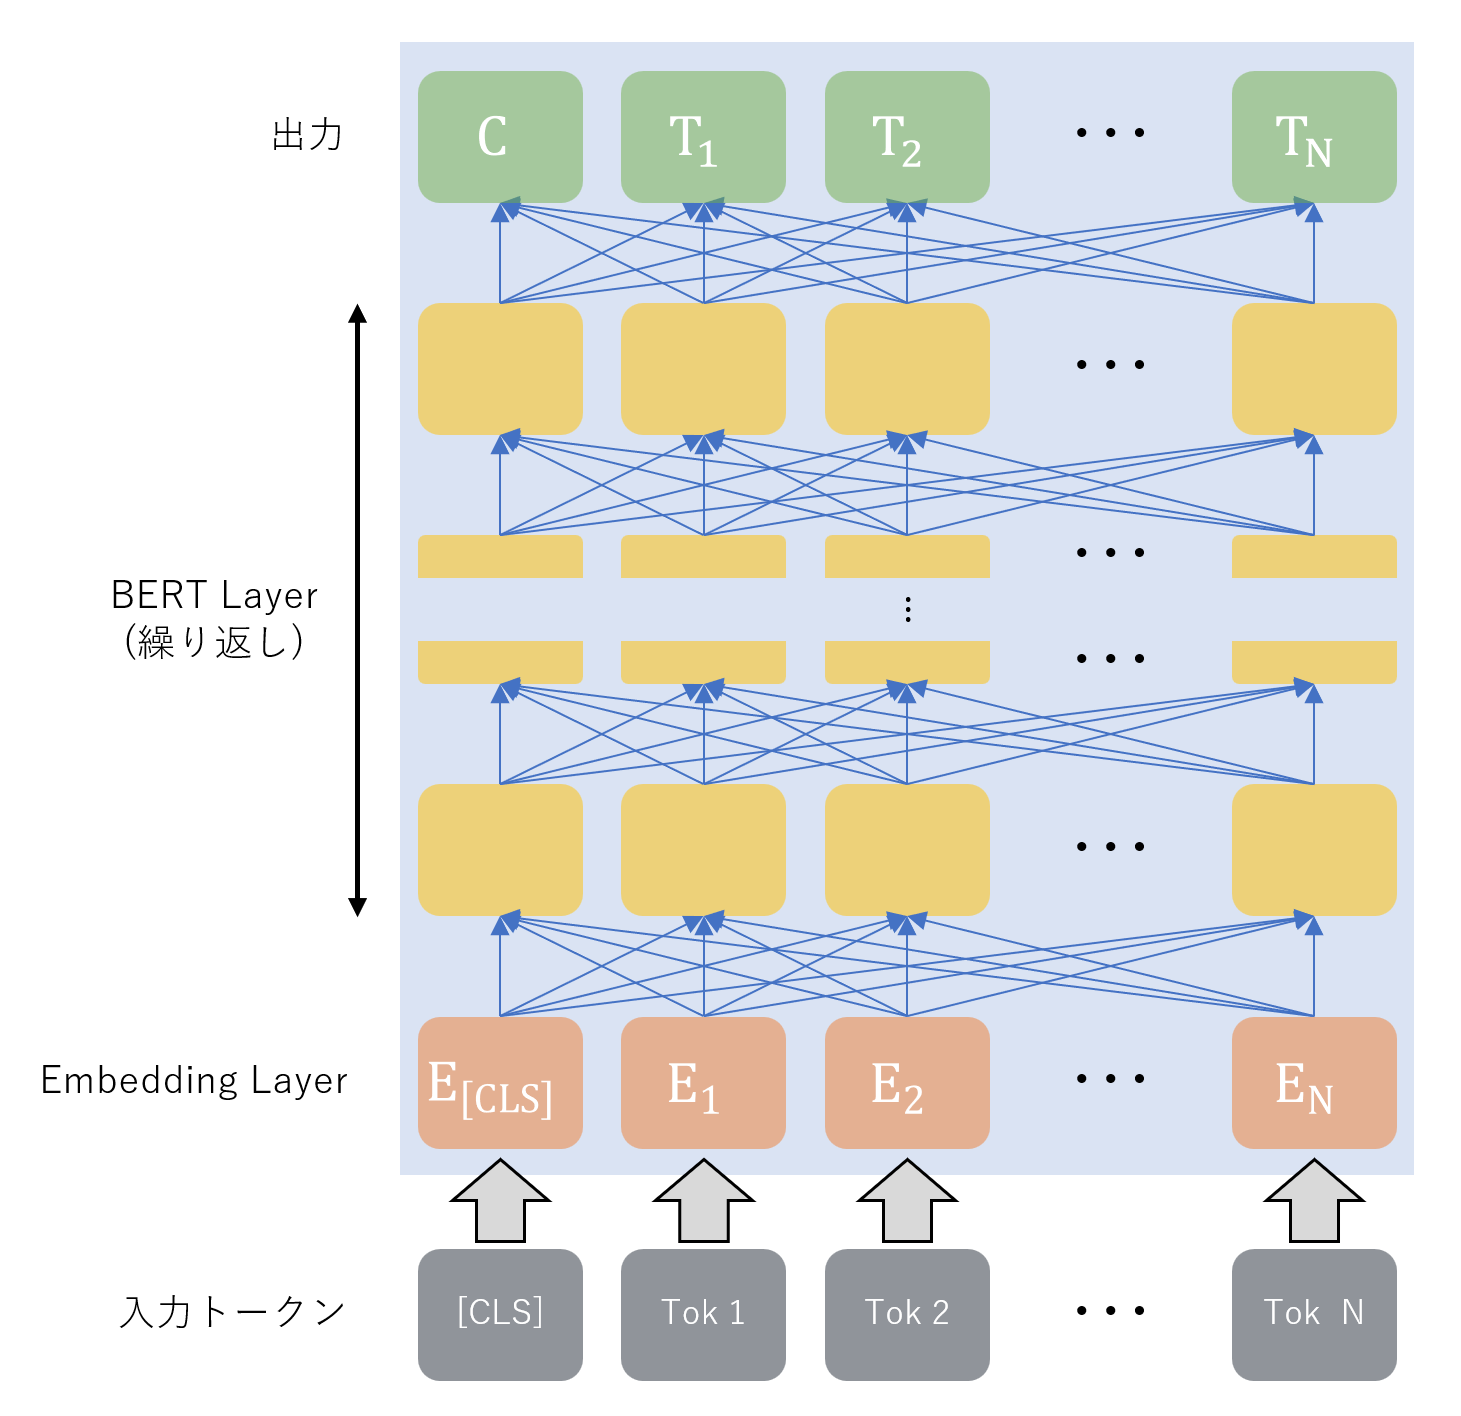
\includegraphics[width=\linewidth]{./figure/bert.png}
			\caption{BERTの概要図}
			\label{fig:bert}
		\end{figure}

	\subsection{BERTから得られる単語分散表現}
		BERTから取得できる単語分散表現の特徴の一つとして,
		同一の単語であっても用いられる文脈によって
		分散表現が変化することが挙げられる.

		例えば,"bank"という単語について考えたとき,
		まったく同じスペルでも文脈に応じて「銀行口座」という意味にも
		「土手」といった意味にもなる.
		Word2Vec等の単語分散表現では,単語に対して分散表現を1対1で対応付けるため,
		こういった多義性を表現することができず,すべて同じ出力となる.
		しかしBERTでは,Traosformer EncoderからなるBERT Layerモジュールを繰り返し通すことで
		単語が持つ多義性を分散表現へ反映させることができると考えられている.

		以下,分散表現が多義性を反映していることを確認する簡単な実験\cite{pytorch_advanced}について述べる.
		"bank"という単語を用いた3つの文章を以下に示す.
		\begin{enumerate}
			\item I accessed the bank account.
			\par 日本語訳)銀行口座にアクセスしました.
			\item He transferred the deposit money into the bank account.
			\par 日本語訳)彼は敷金を銀行口座に振り込みました.
			\item We play soccer at the bank of the river.
			\par 日本語訳)土手でサッカーをします.
		\end{enumerate}
		
		文1,文2では"bank"を「銀行口座」という意味で用いているが,
		文3では"bank"を「土手」という意味で用いている.
		入力はEmbedding Layerから得られる"bank"のトークンに
		一対一で対応した分散表現であるが,
		BERT Layerを繰り返し通すことで,
		この分散表現が周囲の単語の影響を受けながら変化していくことになる.
		各文章の"bank"に対応する出力ベクトルの間でコサイン類似度を算出すると
		以下の表\ref{table:bank_compare}のようになる.
		\begin{table}[H]
			\centering
			\caption{各文章の"bank"についての出力ベクトルの類似度比較}
			\label{table:bank_compare}
			\begin{tabular}[H]{|c|c|}
				\hline
				& cos類似度 \\
				\hline
				文1と文2(同じ意味) & 0.8796 \\
				文1と文3(異なる意味) & 0.4814\\
				\hline
			\end{tabular}
		\end{table}
		% \begin{itemize}
		% 	\item 文1の"bank"と文2の"bank"の類似度 : 0.8796
		% 	\par (どちらも「銀行口座」の意味)
		% 	\item 文1の"bank"と文3の"bank"の類似度 : 0.4814
		% 	\par (文1は「銀行口座」,文3は「土手」の意味)
		% \end{itemize}
		
		このように,"bank"という単語を異なる文章で用いたとしても,
		同じ意味で用いているもの同士であれば,出力ベクトルは類似した出力となる.
		それに対して,"bank"という単語を異なる意味で用いている文章で比較をすると,
		入力としては同じ単語であるにもかかわらず出力ベクトルの類似度は低下する.
		このような結果から,BERTから取得できる単語分散表現には
		文脈考慮性があるということが示唆されている.





\chapter{文脈を考慮した一般単語感情推定手法}	

	\section{全体の概要}
	単語に対して想起される感情は,その単語が用いられる文脈に応じて変化するといえる.
	例えば「ドライブ」という単語について考えたとき,
	「海までドライブに行って気持ちよかった.」という文脈で用いられた場合には,
	喜などのポジティブな感情を想起すると考えられる.
	しかし,「ドライブで事故にあってしまった」という文脈で用いられた場合には,
	怖などのネガティブな感情を想起すると考えられる.
	このように,単語に対して想起される感情は文脈によって異なる.
	本手法では,単語から想起される感情を文脈によって変化させる.
	これにより,対話システムに応用するなど,後続のタスクで用いやすい形の
	感情情報を与えることが期待される.

	本手法では,BERTから得られる単語分散表現を活用することにより,
	同一単語に対しても文脈に応じて出力される感情ベクトルを変化させる.
	具体的には,BERTの出力する単語分散表現が文脈に応じて変化する性質を利用し,
	出力される感情ベクトルを変化させている.
	図\ref{fig:flowchart}は提案手法の流れを示したものである.
	\begin{figure}[H]
		\centering
		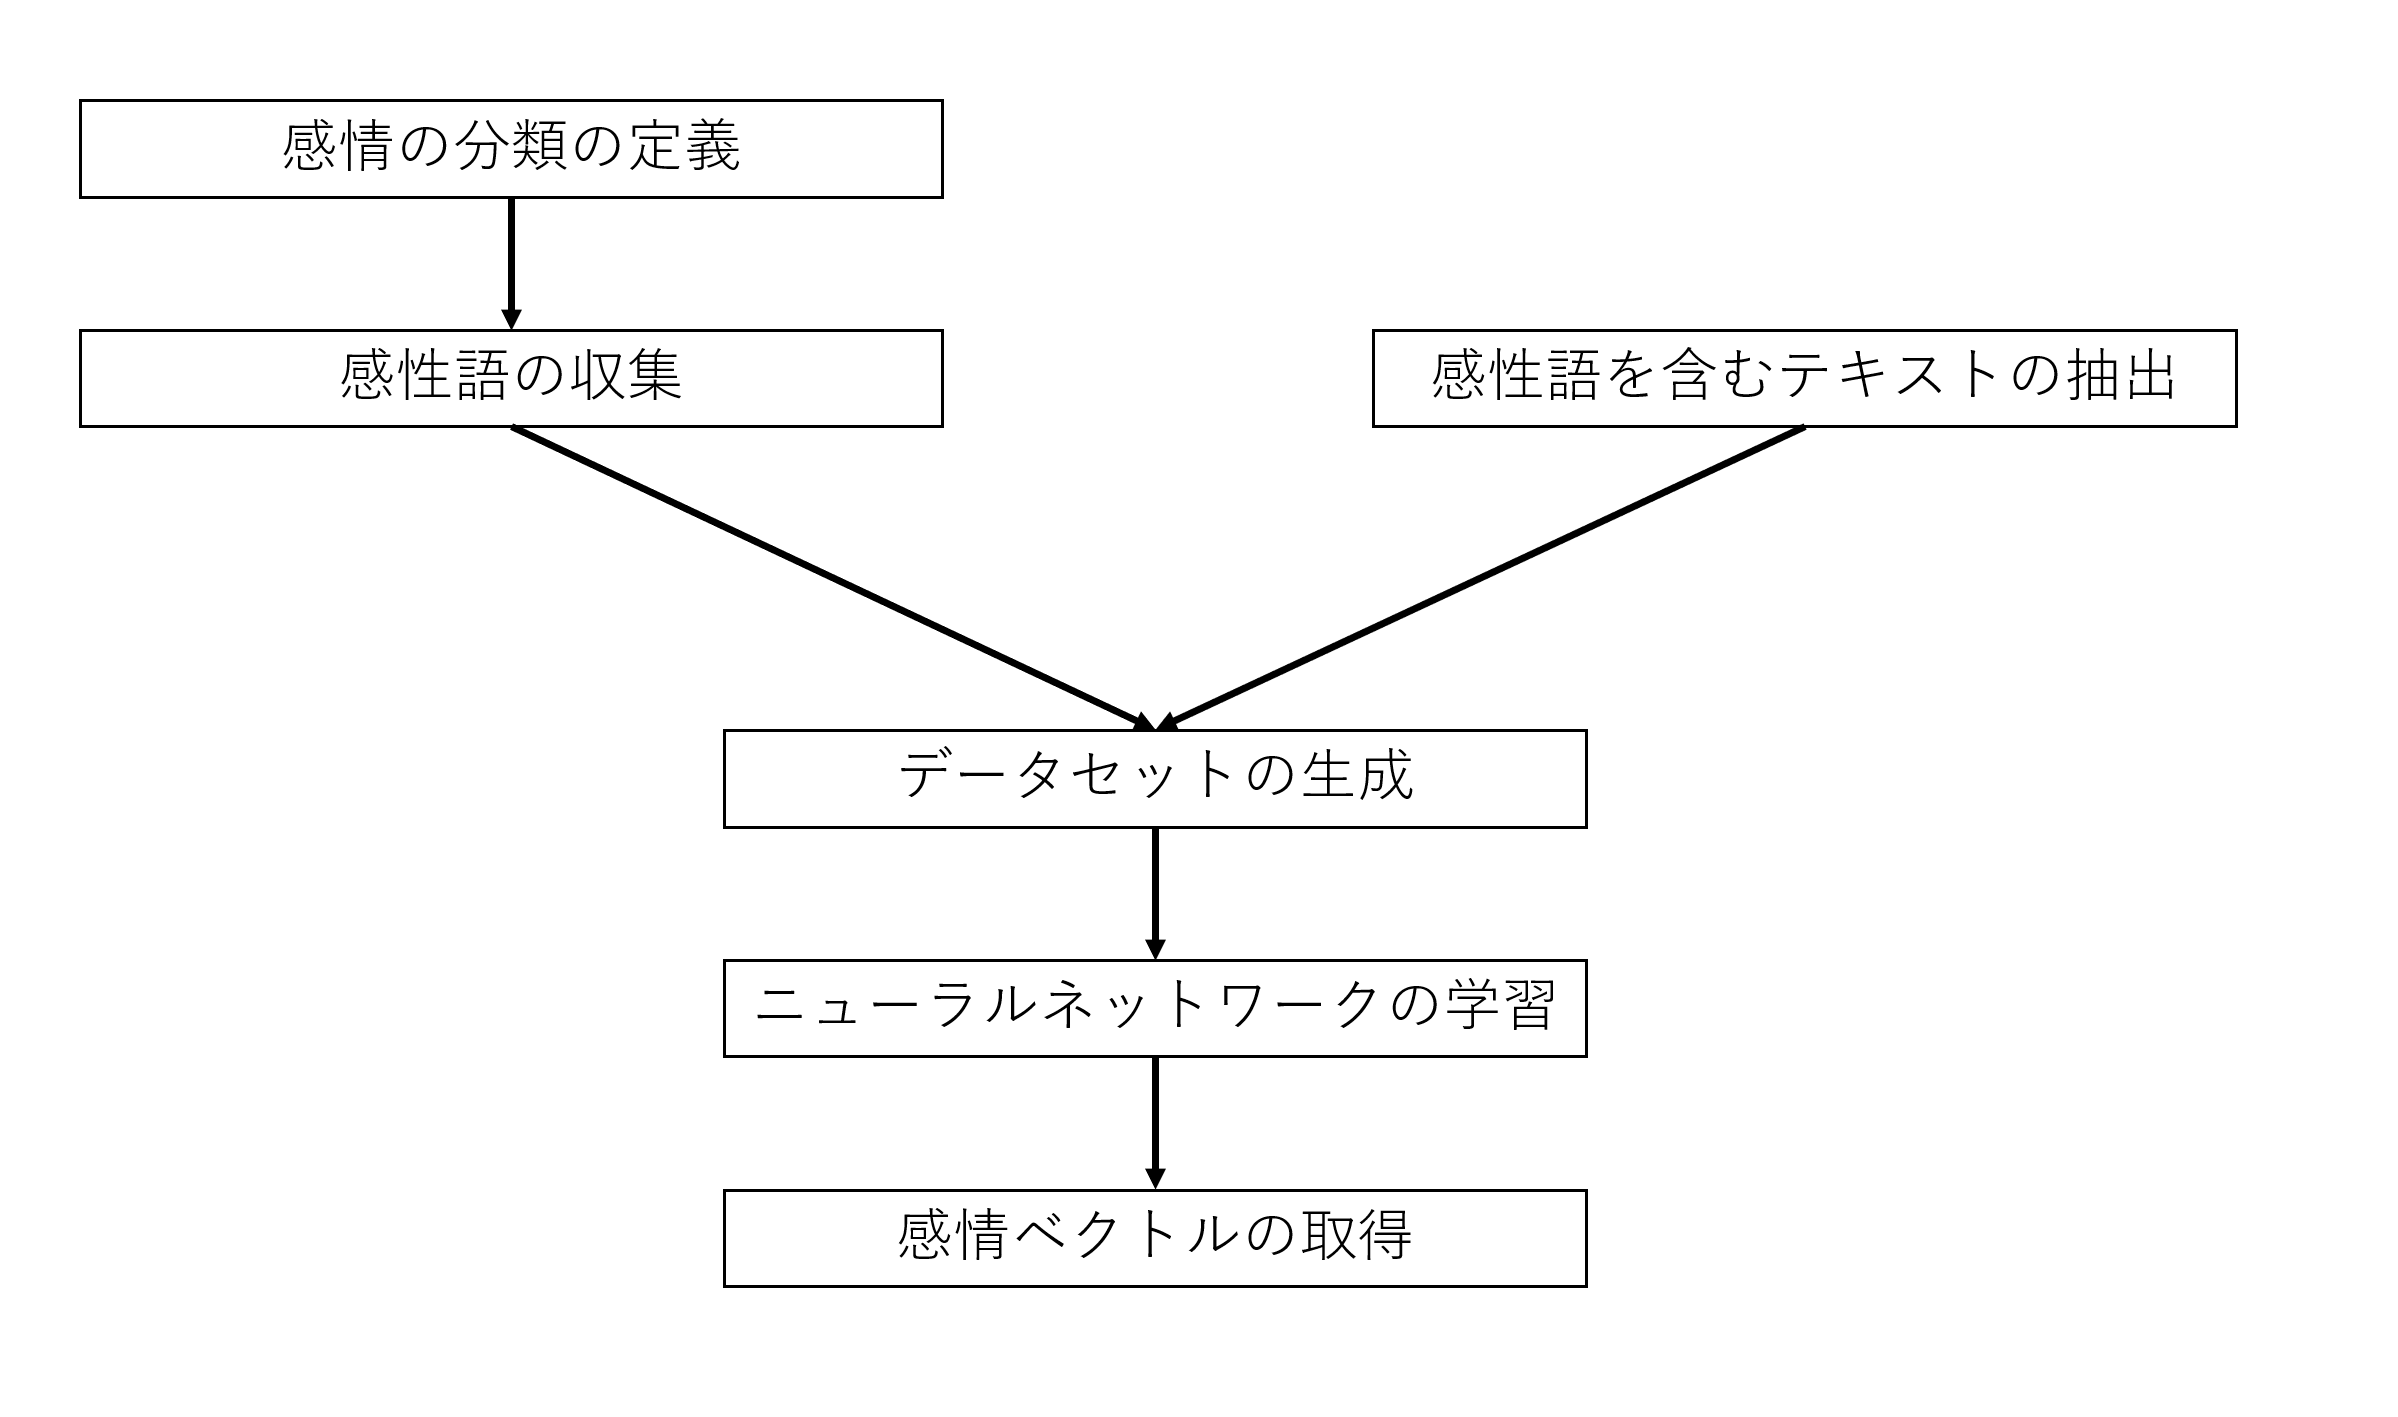
\includegraphics[width=\linewidth]{./figure/flowchart.png}
		\caption{提案手法の流れ}
		\label{fig:flowchart}
	\end{figure}
	分散表現と感情ベクトルを対応付けるに当たり,
	感情表現辞典\cite{kanjou_hyogen_jiten}から取得できる単語である感性語と
	その感情情報を利用する.
	Word2Vecの学習を行う上でもとになっている分布仮説の考え方を応用し,
	感性語の感情が周囲の単語に影響を与えるという仮説のもとでデータセットを生成した.
	分散表現から感情ベクトルへの変換には非常にシンプルなニューラルネットワークを用い,
	学習を行った.
	本手法で作成したシステムでは,文章を入力することによりそれを構成している単語の感情ベクトルを
	入力文の文脈を考慮した上で出力することができる.
	また,入力がBERTの分散表現としたことで,感情ベクトルを出力可能な単語数は
	BERTが扱うことのできる語彙数と一致し,従来の辞書構築型アプローチと比べると
	対応可能語彙数は大幅に増加している.
	以下,本手法の流れについて述べる.



	\section{提案手法の流れ}
		図\ref{fig:whole_image}は,入力されたテキストからそれを構成する各単語の感情情報を抽出するまでの
		全体的な処理の様子を示したものである.
		以下,これに沿って提案手法を説明する.

		\begin{figure}[H]
			\centering
			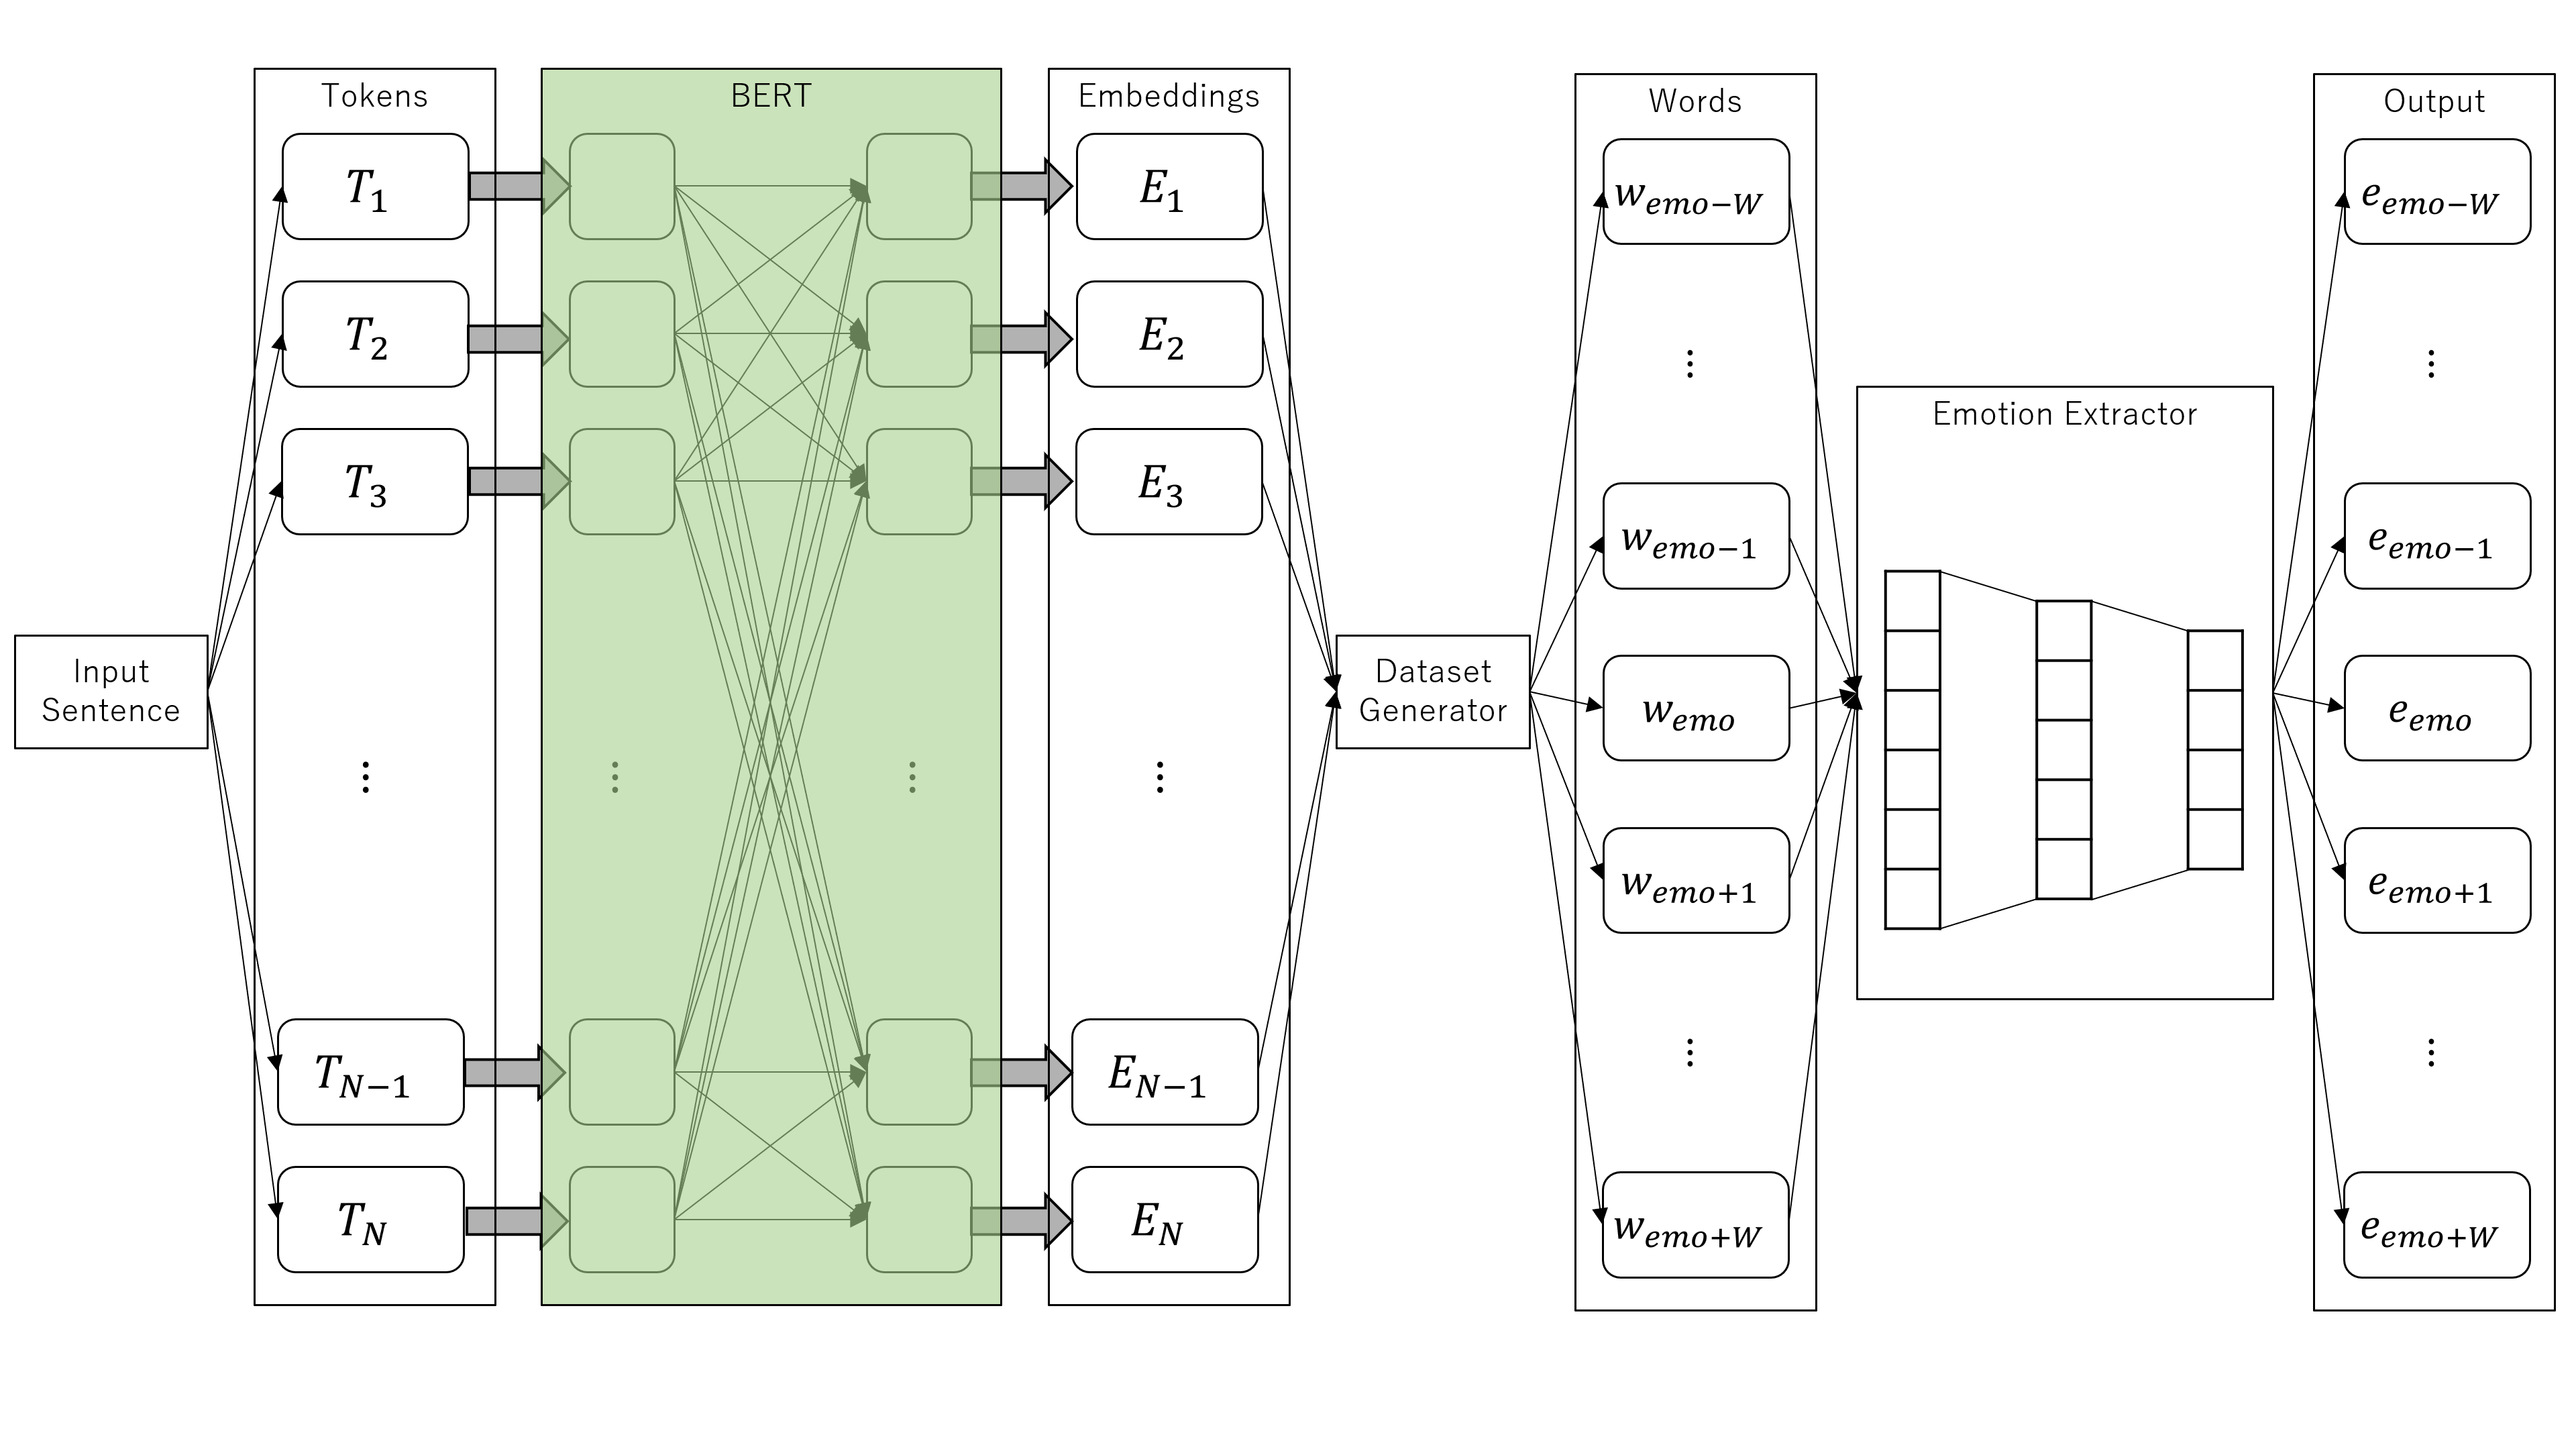
\includegraphics[width=\linewidth]{./figure/whole_image.png}
			\caption{感情情報の抽出における処理の様子}
			\label{fig:whole_image}
		\end{figure}

		\subsection{感情の分類方法の決定}
			本手法における感情分類の方法として,感情表現辞典\cite{kanjou_hyogen_jiten}で
			取得できる感情ベクトルに合わせた10次元の感情分類を採用している.
			各感情は「喜,怒,哀,怖,恥,好,厭,昂,安,驚」である.
			これらの感情は,日本語における言語表現の観点から決められたものである.

		\subsection{感性語の収集}
			感情表現辞典には,各感情を表す単語および熟語が2278語収録されている.
			各単語に対し,該当する感情に1,該当しない感情に0を割り振った10次元の感情ベクトルを
			対にしてリスト化した.
			いくつか例を示す.
			\begin{itemize}
				\item 「めでたい」
				\par $$(喜, 怒, 哀, 怖, 恥, 好, 厭, 昂, 安, 驚)=(1, 0, 0, 0, 0, 0, 0, 0, 0, 0)$$
				\item 「恐ろしい」
				\par $$(喜, 怒, 哀, 怖, 恥, 好, 厭, 昂, 安, 驚)=(0, 0, 0, 1, 0, 0, 0, 0, 0, 0)$$
			\end{itemize}

			また,これらの感性語の中に多数の感情に1が割り振られた単語(以下,感性多義語とよぶ)が存在する.
			感性多義語の例を以下に示す.
			\begin{itemize}
				\item 「気持ち」
				\par $$(喜, 怒, 哀, 怖, 恥, 好, 厭, 昂, 安, 驚)=(1, 1, 0, 0, 0, 0, 1, 0, 1, 0)$$
				\item 「涙」
				\par $$(喜, 怒, 哀, 怖, 恥, 好, 厭, 昂, 安, 驚)=(1, 0, 1, 0, 0, 0, 1, 1, 0, 0)$$
				\item 「思い」
				\par $$(喜, 怒, 哀, 怖, 恥, 好, 厭, 昂, 安, 驚)=(0, 0, 1, 0, 0, 1, 1, 0, 0, 1)$$
			\end{itemize}

			感性多義語には,多数の感情と結びつくような感情ベクトルが与えられるが,
			あらゆる文脈でこれら全ての感情を想起するようなケースは考えにくい.
			つまり,感性多義語については,感情表現辞典で与えられたベクトルをそのまま出力するだけでなく,
			文脈に応じて適切な感情の出力を強調し,不適切な感情の出力を抑えることが求められる.
			
			なお,感情表現辞典に掲載された単語および熟語のうち,
			分かち書きで2単語以上に分かれてしまうものについては
			リストから除外を行った.
			これは,分かち書きで分解された各要素のうち,どの部分に感情情報があるのかを
			判断するのが難しいためである.
			この際,分かち書きには,形態素解析エンジンのMeCab\cite{mecab}を用いた.
			\begin{table}[H]
				\caption{感情表現辞典から取得した感性語の例}
				\label{table:kansei_words}
				\centering
					\begin{tabular}{cc}
						\hline
						感情 & 感性語の例 \\
						\hline \hline
						喜 & めでたい,歓喜,感謝,誇り,$\cdots$ \\
						怒 & 腹立たしい,激怒,憤り,反感,$\cdots$ \\
						哀 & 悲哀,哀悼,嘆き,泣き別れ,$\cdots$ \\
						怖 & 不気味,恐ろしい,震えあがる,戦慄,$\cdots$ \\
						恥 & 照れる,生き恥,羞恥心,赤面,$\cdots$ \\
						好 & 人情,愛する,憧れる,お気に入り,$\cdots$ \\
						厭 & 不快,嫌い,憎しみ,残念,$\cdots$ \\
						昂 & 焦る,緊迫,ときめく,激情,$\cdots$ \\
						安 & 安心,和やか,落ち着く,悠長,$\cdots$ \\
						驚 & たまげる,驚愕,呆然,以外,$\cdots$ \\
						\hline
					\end{tabular}
				\end{table}

		\subsection{感性語を含むテキストデータの取得}
			学習用データセットを作成するにあたり,大量のテキストデータを必要とする.
			しかし,このテキストデータセット自体には感情にかかわるラベル付けがなされている必要はない.
			まず,テキストデータセットを1文ずつに分解したうえで,MeCabによる分かち書きを行い,
			文を構成する各単語の原型のリストを生成した.
			このリスト内に感性語が含まれているような文だけを抜粋し,
			図\ref{fig:whole_image}における"Input Sentece"に対応する
			学習用データセット作成のための入力文とした.

		\subsection{データセットの生成}
			感性語を含むテキストをBERTに入力するにあたり,BERTのトークナイザで入力文をトークン化する.
			これは図\ref{fig:whole_image}の"Input Sentence"から"Tokens"への変換に対応する.
			BERTのトークナイザはMeCabによる形態素解析とwordpieceアルゴリズムによるサブワード分割により構成されている.
			トークン化されたテキストをBERTに入力すると,図\ref{fig:whole_image}の"Embeddings"に対応する,
			各トークンの分散表現を取得することができる.

			以下,図\ref{fig:whole_image}の"Dataset Generator"に対応する処理について述べる.
			まず,感性語の周辺単語の収集を行う.
			ウィンドウサイズを$W$としたとき,感性語の前後それぞれ$W$個の単語を収集する.
			なお,サブワード分割されたトークンは結合した状態でウィンドウサイズをカウントする.
			その際には,名詞,形容詞,形容動詞,動詞以外はカウント対象外とした.
			また,名詞のうち,代名詞,接尾語,非自立語,数詞についても除外を行った.
			これらの単語が感情情報を持つとは考えにくいためである.

			感性語が持っている感情ベクトルを図\ref{fig:whole_image}の"Words"に対応する,
			ウィンドウサイズ内の単語すべてに付与することにより,
			学習用データセットは生成されることになる.
			つまり,ウィンドウサイズ内のトークンに対応する分散表現と感情ベクトルのペアが1件のデータ
			ということになる.
			以下に例を示す.

			図\ref{fig:token_processing}は,
			入力テキストとして「道の真ん中で転んでしまい恥ずかしかったので,走ってその場を立ち去った」
			という文章を与えたときのトークン処理の様子である.
			この文章をBERTへ入力するために,まずトークン化を行う.
			ここで,"\#\#"で始まるトークンが存在するが,これは分かち書きの後さらに
			サブワード分割がなされたために生じるトークンである.
			よって,品詞による判別を行うためにはサブワード分割されたトークンを結合する必要性がある.
			サブワード結合状態での分割単位で品詞を調査し,
			ウィンドウサイズのカウント対象となるトークン列を絞り込む.
			\begin{figure}[H]
				\centering
				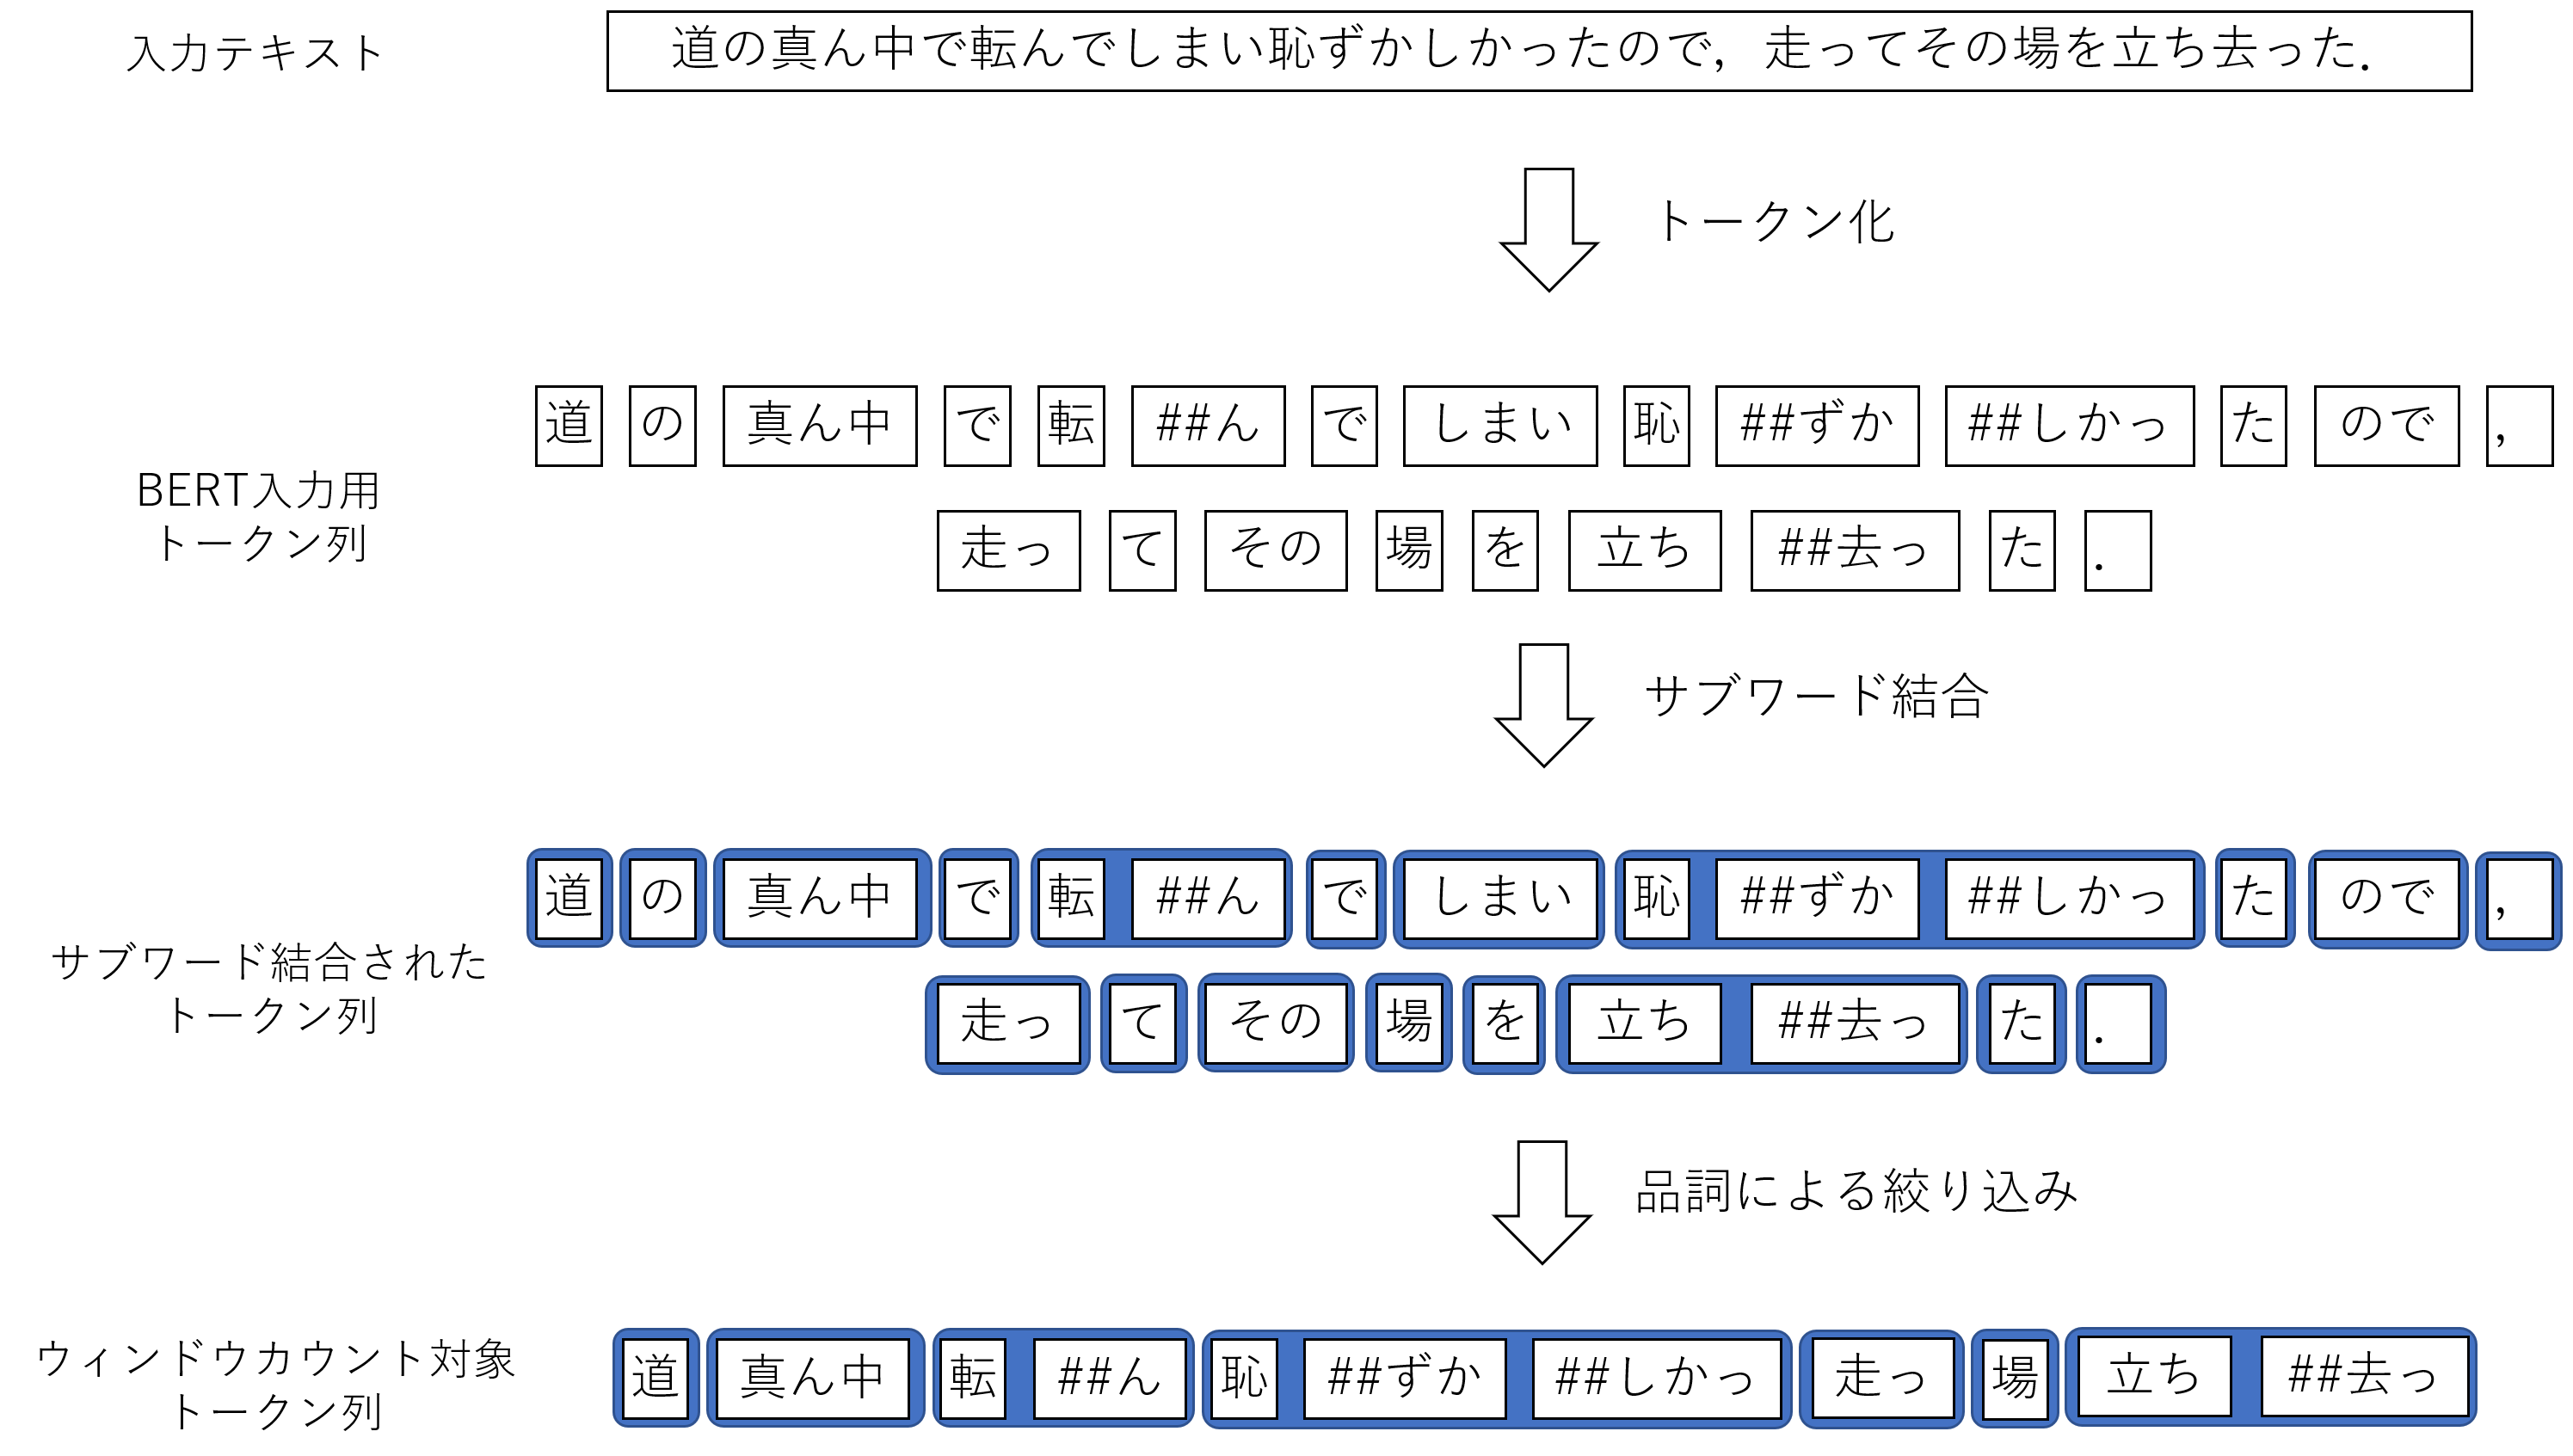
\includegraphics[width=\linewidth]{./figure/token_processing.png}
				\caption{入力文から生成されるトークンの処理の様子}
				\label{fig:token_processing}
			\end{figure}
			これらのトークン列のうち,「恥 \#\#ずか \#\#しかっ」の原型である「恥ずかしい」が
			感性語となる.
			よって,以下のような感情ベクトルを感情表現辞典から取得することができる.
			$$(喜, 怒, 哀, 怖, 恥, 好, 厭, 昂, 安, 驚)=(0, 0, 0, 0, 1, 0, 0, 0, 0, 0)$$
			ウィンドウサイズを3としたとき,「恥 \#\#ずか \#\#しかっ」の前後それぞれ3つずつの
			トークン列へ同様の感情ベクトルを付与することになる.
			図\ref{fig:make_dataset_window}は,この様子を図式化したものである.
			\begin{figure}[H]
				\centering
				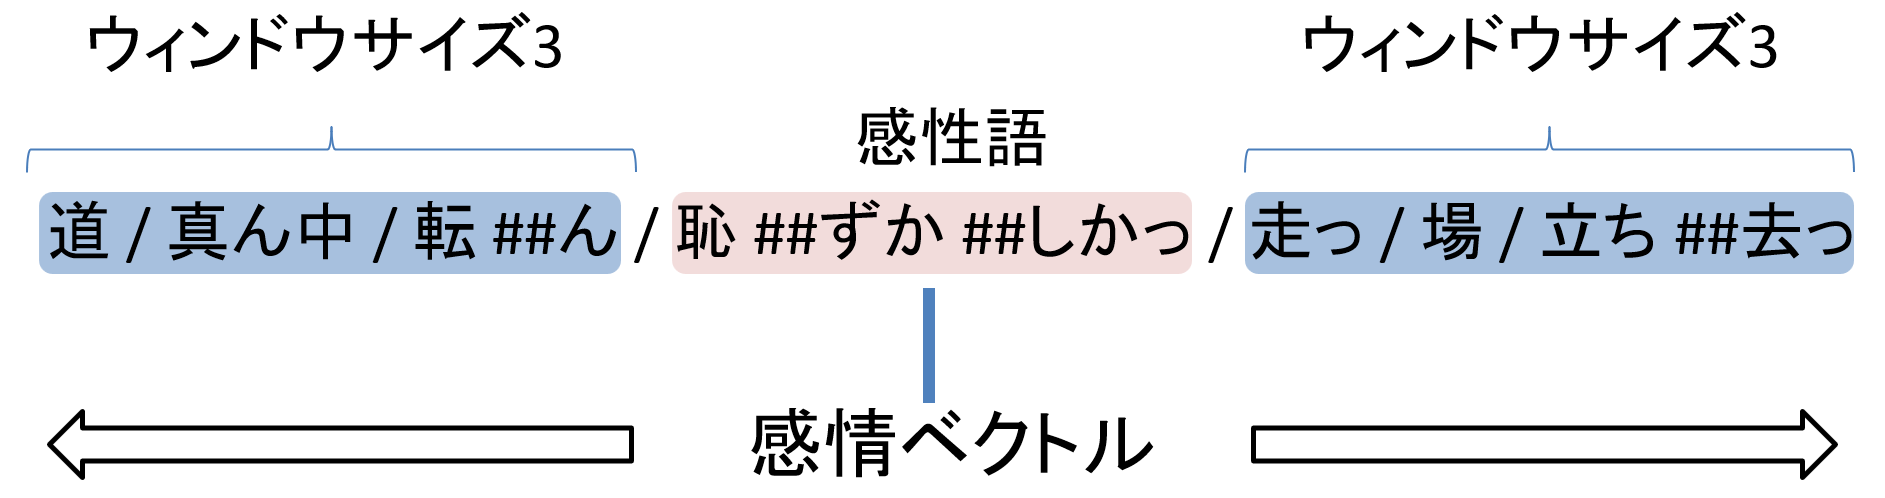
\includegraphics[width=\linewidth]{./figure/dataset_make_window.png}
				\caption{中心の感性語が持つ感情ベクトルを周辺単語へ付与する様子}
				\label{fig:make_dataset_window}
			\end{figure}


			また本手法ではデータセット生成に当たり,
			与える感情ベクトルについて感性語と周辺単語の距離に応じた重み付けを行った。
			感性語との距離が離れるほど、与えられる感情ベクトルの強度が弱くなる。
			これは,感性語ではない一般単語が感性語と同等の強度でその感情を想起するわけではない,
			という仮説に基づくものである.
			表\ref{table:vector_weaken}は最小値を0.5とした上で感性語との距離に応じて
			等間隔に値が小さくなるよう感情ベクトルを付与している様子を表している.
			\begin{table}[H]
				\centering
				\caption{感性語からの距離に応じて感情ベクトルの強度を弱める様子}
				\label{table:vector_weaken}
					\begin{tabular}{cccccccccc}
						\hline
						感性語との距離 & -4 & -3 & -2 & -1 & 0 & +1 & +2 & +3 & +4 \\
						\hline
						ベクトル強度 & 0.5 & 0.625 & 0.75 & 0.875 & 1.0 & 0.875 & 0.75 & 0.625 & 0.5 \\
						\hline
					\end{tabular}
			\end{table}

		\subsection{ニューラルネットワークの学習}
			本手法では,BERTが出力するトークンの分散表現から感情ベクトルを出力するために,
			非常にシンプルなニューラルネットワークを採用し,学習を行った.
			これは図\ref{fig:whole_image}の"Emotion Extractor"に対応する.
			以下の図\ref{fig:network}は、用いるネットワークを図式化したものである。
			\begin{figure}[H]
				\centering
				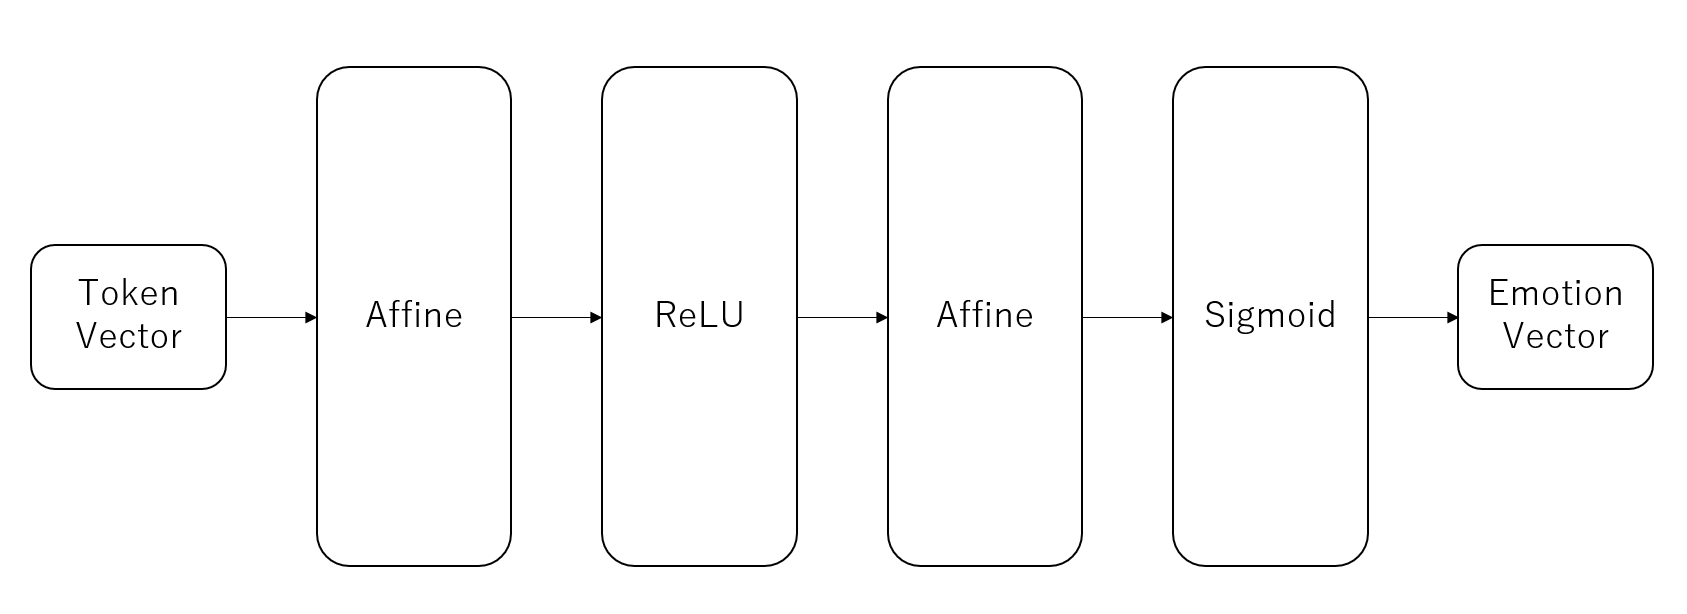
\includegraphics[width=\linewidth]{./figure/network.png}
				\caption{ニューラルネットワークの構造}
				\label{fig:network}
			\end{figure}
			具体的には,入力層が768次元の分散表現,出力層が10次元の感情ベクトルとなるため,
			400次元の中間層を設けた3層のニューラルネットワークを学習させた.
			中間層の活性化関数はReLU関数\cite{relu}とし,
			出力層にはSigmoid関数をかけ、0から1の値へ変換を施している。
			ReLU関数,Sigmoid関数はそれぞれ以下の式で示される.
			\begin{equation}
				ReLU(x)=
				\left\{
				\begin{alignedat}{2}
					x\;\;\;(x>0) \\
					0\;\;\;(x\leqq0)
				\end{alignedat}
				\right.
			\end{equation}
			\begin{equation}
				Sigmoid(x)=\frac{1}{1+e^{-x}}
			\end{equation}

			この時出力された10次元のベクトルが,
			データセットに与えられた感情ベクトルに近づくよう学習を行う.
			損失関数は最小二乗誤差とした.

		\subsection{感情ベクトルの取得}
			以上のようにして学習したネットワークに,BERTから得られたトークンの分散表現を入力することにより,
			入力文全体の文脈を踏まえた感情ベクトルを出力することができる.
			出力対象単語は,データセット作成時のウィンドウサイズカウント対象になる単語と
			同等の条件を満たすものに絞っている.
			また,サブワードに別れてしまう単語については,
			それぞれのトークンに対して出力される感情ベクトルの平均値をまとめて出力する.

			本手法では,出力に正規化を行わなかった.
			その理由としては,感情表現辞典から得られる感情ベクトルには
			複数の感情のラベルがついた単語が存在していること,
			1感情に対してだけわずかに値が出力されるようなケースでは
			その値が極端に大きくなってしまう可能性があることが挙げられる.

\chapter{評価実験}

\label{chap:evaluation}

\section{実験環境}
	\subsection{データセット生成}
		感性語の抽出を行うにあたり,感情表現辞典に掲載された情報を活用する.
		感情表現辞典に収録されている単語と熟語の合計2278語のうち,
		MeCabで分かち書きを行うことで複数単語に別れてしまうものを除くと,
		1245語となる.
		なお,MeCabの辞書にはipadicを用いた.
		本実験におけるデータセット生成では,これらを感性語とする.

		データセット生成のためのテキストデータには
		Wikipedia\cite{wikipedia}のテキストに前処理を施した状態で公開されている
		Wiki-40B\cite{wiki-40b}データセットの日本語版を用いる.
		1文ずつに分割し,感性語を含む文章のみを抽出した.
		それぞれの文章の数は以下の表\ref{table:wiki40b_sentence}の通りである.
		\begin{table}[H]
			\centering
			\caption{wiki-40bデータセットから得られる文章の数}
			\label{table:wiki40b_sentence}
			\begin{tabular}{cccc}
				\hline
				& Train & Val & Test \\
				\hline \hline
				全文章 & 12,330,278 & 677,757 & 678,490 \\
				感性語を含む文章 & 2,337,909 & 128,126 & 128,698 \\
				\hline
			\end{tabular}
		\end{table}
		% $Train/Val/Test=12,330,278/677,757/678,490$となった.
		% これらのうち,感性語を含む文は
		% $Train/Val/Test=2,337,909/128,126/128,698$となった.
		本実験では,ウィンドウサイズ$W=3$とし,感性語の周辺単語を収集した.
		このBERTが出力した分散表現と感情ベクトルがペアになった
		データセットのサイズは,
		% $Train/Val/Test=20,154,529/1,104,904/1,108,482$
		% となった.
		以下の表\ref{table:bert_to_emo_size}の通りである.
		\begin{table}[H]
			\centering
			\caption{作成したデータセットのサイズ}
			\label{table:bert_to_emo_size}
			\begin{tabular}{ccc}
				\hline
				Train & Val & Test \\
				\hline \hline
				20,154,529 & 1,104,904 & 1,108,482 \\
				\hline
			\end{tabular}
		\end{table}
		なお,用いたBERTモデルはHugging Face\cite{huggingface}で東北大学が公開している
		cl-tohoku/bert-base-japanese-whole-word-masking\cite{cl-tohoku}である.

	\subsection{ニューラルネットワークの学習条件}
		入力が768次元の単語分散表現で,出力が10次元の感情ベクトルとなる.
		本実験では図\ref{fig:network}で示すような,中間層を400次元とした
		非常にシンプルな3層のニューラルネットワークを構築し,
		生成したデータセットを用いて学習を行った.
		\begin{figure}[H]
			\centering
			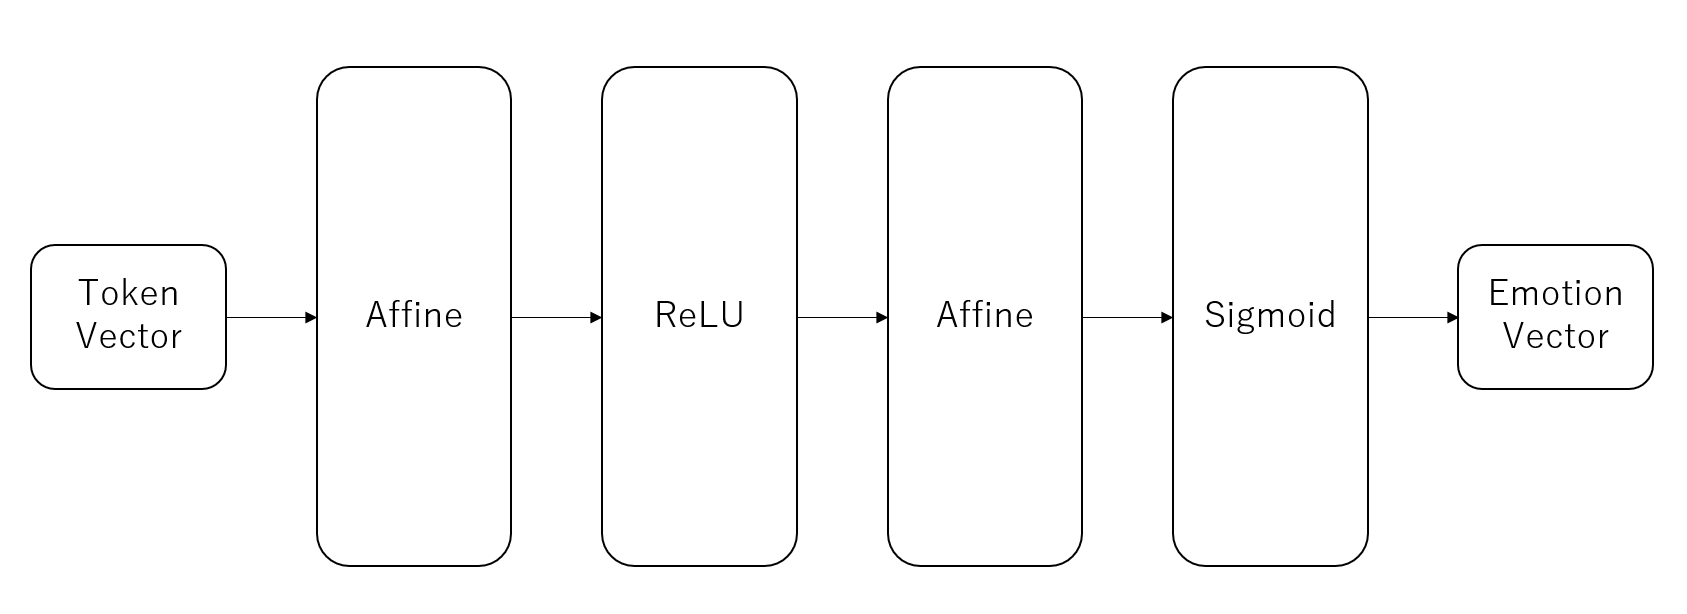
\includegraphics[width=\linewidth]{./figure/network.png}
			\caption{ニューラルネットワークの構造}
			\label{fig:network}
		\end{figure}
		中間層の活性化関数はReLU関数とし,
		出力層にsigmoid層を通すことにより,0以上1以下の値に変換する.
		この時,出力された10次元のベクトルが,データセットに与えられた
		感情ベクトルに近づくよう学習を行うことになる.
		損失関数は最小二乗誤差とし,Adamにより学習率$1\times10^{-3}$で最適化を行った.
		エポック数については,Early Stoppingで5回以上validation lossが更新
		されなかった段階で学習を終了させた.
		
	\subsection{比較手法}
		本手法と比較するためのベースライン手法として,BERT Layerを通す前の
		Embedding Layerによる分散表現をネットワークの入力とした場合を設定する.
		BERT Layerを通すことにより,Transformerによる周りの単語の影響を加味することになる.
		今回設定したベースラインではEmbedding Layerによる
		分散表現を利用することで周辺単語の影響が含まれないことになる.
		また、感性語の周辺単語に与える感情ベクトルについて
		距離に応じた重み付けを行うことによる効果を確認するため,
		重み付けを行うBERT+weight,行わないBERTに分けて実験を行う.

\section{感情ベクトルの生成例}
	入力文に対する各単語の感情ベクトル出力例を以下に示す.
	\subsection{「仕事は人生を豊かにしてくれる.」に対する出力}
		\begin{figure}[H]
			\begin{tabular}{cc}
				\begin{minipage}[t]{0.45\hsize}
					\centering
					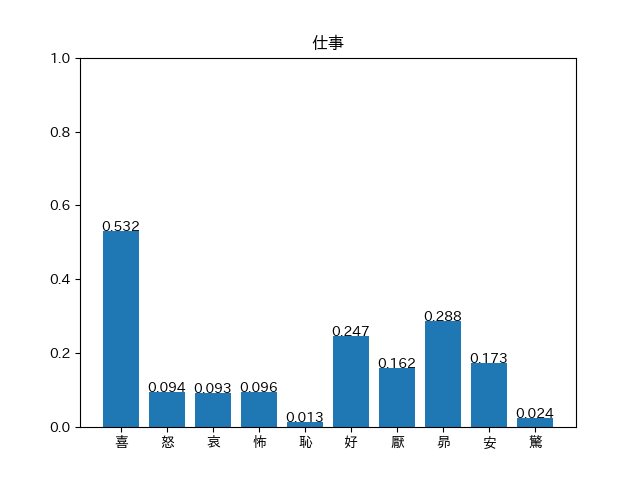
\includegraphics[keepaspectratio, scale=0.45]{./figure/output/Q01/001.png}
					\subcaption{「仕事」に対する感情ベクトル}
				\end{minipage} &
				\begin{minipage}[t]{0.45\hsize}
					\centering
					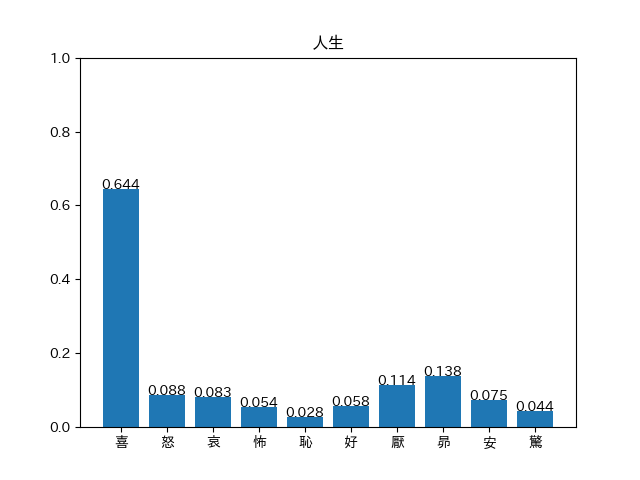
\includegraphics[keepaspectratio, scale=0.45]{./figure/output/Q01/002.png}
					\subcaption{「人生」に対する感情ベクトル}
				\end{minipage} \\
				\begin{minipage}[t]{0.45\hsize}
					\centering
					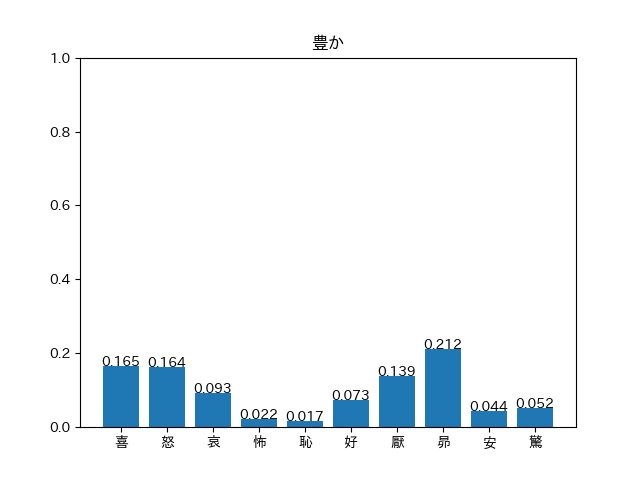
\includegraphics[keepaspectratio, scale=0.45]{./figure/output/Q01/003.png}
					\subcaption{「豊か」に対する感情ベクトル}
				\end{minipage} &
				\begin{minipage}[t]{0.45\hsize}
					\centering
					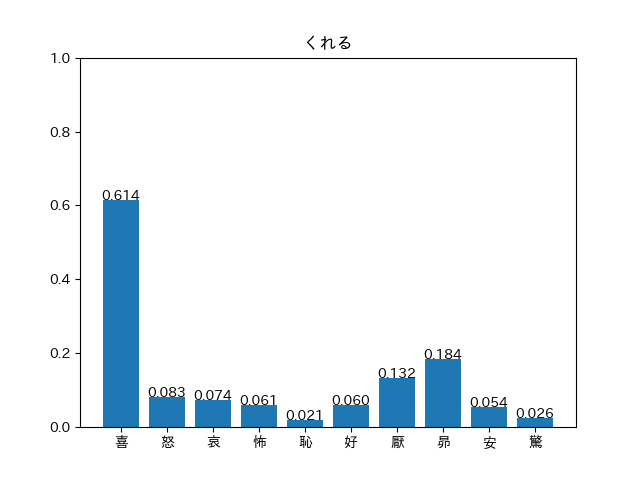
\includegraphics[keepaspectratio, scale=0.45]{./figure/output/Q01/004.png}
					\subcaption{「くれる」に対する感情ベクトル}
				\end{minipage} \\
			\end{tabular}
			\caption{「仕事は人生を豊かにしてくれる.」に対する各単語の感情ベクトル}
			\label{fig:output_ex01}
		\end{figure}

	\subsection{「仕事は面倒だし、疲れるから嫌だ。」に対する出力}
		\begin{figure}[H]
			\begin{tabular}{cc}
				\begin{minipage}[t]{0.45\hsize}
					\centering
					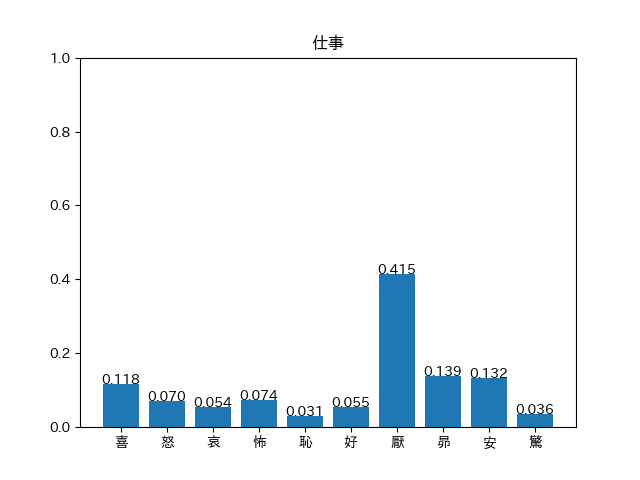
\includegraphics[keepaspectratio, scale=0.45]{./figure/output/Q02/001.png}
					\subcaption{「仕事」に対する感情ベクトル}
				\end{minipage} &
				\begin{minipage}[t]{0.45\hsize}
					\centering
					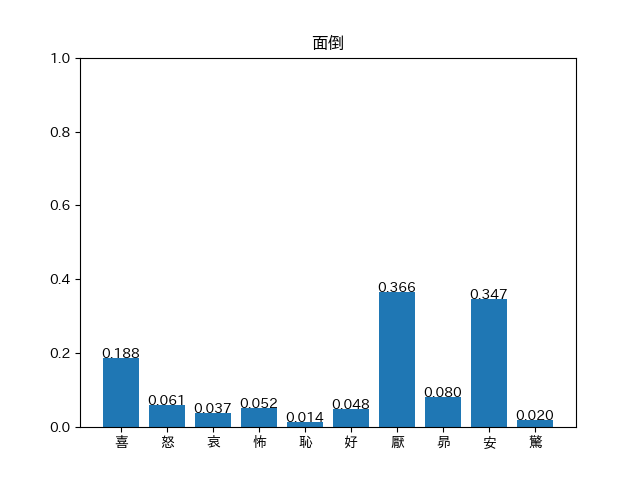
\includegraphics[keepaspectratio, scale=0.45]{./figure/output/Q02/002.png}
					\subcaption{「面倒」に対する感情ベクトル}
				\end{minipage} \\
				\begin{minipage}[t]{0.45\hsize}
					\centering
					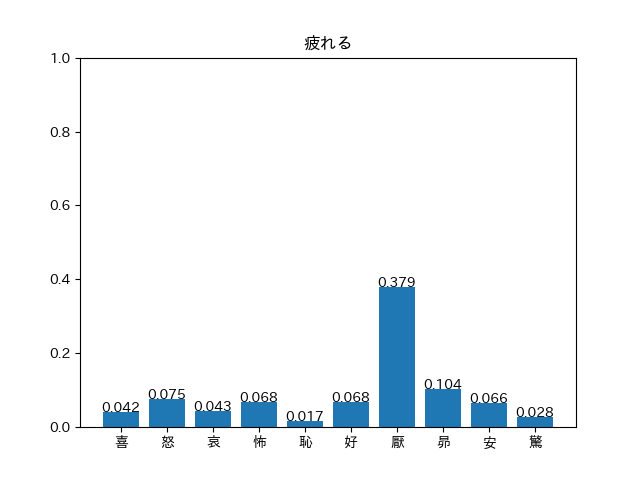
\includegraphics[keepaspectratio, scale=0.45]{./figure/output/Q02/003.png}
					\subcaption{「疲れる」に対する感情ベクトル}
				\end{minipage} &
				\begin{minipage}[t]{0.45\hsize}
					\centering
					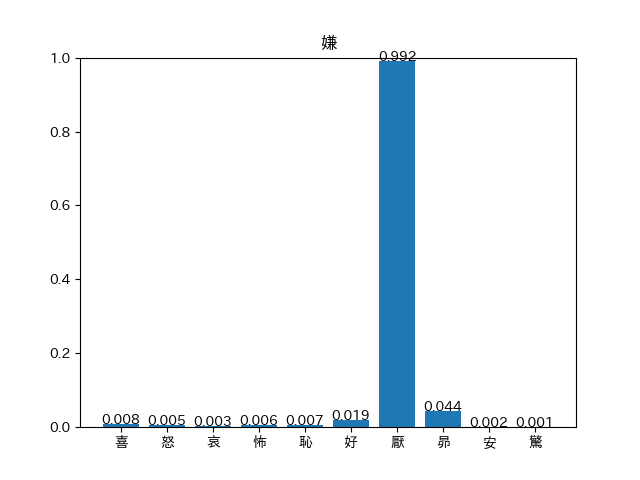
\includegraphics[keepaspectratio, scale=0.45]{./figure/output/Q02/004.png}
					\subcaption{「嫌」に対する感情ベクトル}
				\end{minipage} \\
			\end{tabular}
			\caption{「仕事は面倒だし、疲れるから嫌だ.」に対する各単語の感情ベクトル}
			\label{fig:output_ex02}
		\end{figure}

		図\ref{fig:output_ex01}ではポジティブな文脈で「仕事」という単語を用いているのに対し,
		図\ref{fig:output_ex02}ではネガティブな文脈で「仕事」という単語を用いている.
		それぞれの「仕事」に対する感情ベクトルを比較すると,
		文脈に応じてその出力が変化していることがわかる.

\section{単語の感情推定の妥当性に関する評価実験}
	\subsection{実験設定}
		本実験では,本システムにより出力された単語の感情ベクトルが
		人間の想起する感情のイメージと合致しているのかを検証する.
		単語を一般単語,感性語,感性多義語3つに分け,それぞれ検証を行う.
		実験に先立ち,被験者には表\ref{table:input_word}に示すような特定の単語を用いる文章を生成してもらった.
		\begin{table}[H]
			\centering
			\caption{文章生成時に指定した単語}
			\label{table:input_word}
			\begin{tabular}{|c|c|}
				\hline
				一般単語 & 
				\begin{tabular}{c}
					仕事,学校,試作,軽い,リンゴ,もたらす,\\夏休み,真似,手順,呼び寄せる,果物,石鹸,\\海老,最年長,エアコン,地下道,建て直す,積み重なる
				\end{tabular} \\
				\hline
				感性語 &
				\begin{tabular}{c}
					驚かす,笑み,切ない,恋しい,好む,不満,\\大嫌い,めでたい,侮る,立腹,安らか,感慨,\\心苦しい,名残惜しい,嬉し涙,祝する,叱り付ける,晴れ渡る
				\end{tabular} \\
				\hline
				感性多義語 & 気持ち,思い,涙 \\
				\hline
			\end{tabular}
		\end{table}
		一般単語については,
		各単語につきポジティブな文脈・ネガティブな文脈のそれぞれで生成してもらい,
		合計36文となった.
		感性語については,各単語につき1文ずつ生成してもらい,合計18文となった.
		感性多義語については,各単語につきポジティブな文脈・ネガティブな文脈のそれぞれで複数対
		生成してもらい,合計34文となった.
		以下の表では,単語とその単語を用いた文章の生成例を示している.
		\begin{table}[H]
			\centering
			\caption{特定の単語を用いた生成文の例}
			\label{table:generated_sentences_sample}
			\begin{tabular}{|c|c|c|}
				\hline
				\multirow{2}{*}{一般単語} & \multirow{2}{*}{仕事} & 仕事は人生を豊かにしてくれる. \\
				\cline{3-3}
				& & 仕事は面倒だし、疲れるから嫌だ. \\
				\hline
				感性語 & 驚かす & 兄は私をいきなり驚かした. \\
				\hline
				\multirow{2}{*}{感性多義語} & \multirow{2}{*}{気持ち} & 彼女と話すと楽しい気持ちになる. \\
				\cline{3-3}
				& & 食べ過ぎて気持ちが悪い. \\
				\hline
			\end{tabular}
		\end{table}

		これらの文章をシステムに入力したうえで,
		文章生成時に指定した単語(以下,対象単語とよぶ)
		の感情ベクトルを出力した.
		対象単語について,それが用いられた文脈を考慮した上で想起されるような
		感情を感情ベクトルの形で被験者に予想してもらった.
		システム出力,被験者により予想された感情ベクトルをそれぞれ正規化したうえで,
		Top-1精度,Top-3精度,コサイン類似度を比較する.
		同次元のベクトル$\bold{a},\bold{b}$について,これらのコサイン類似度は
		以下のように計算される.
		\begin{equation}
			cos(\boldsymbol{a},\boldsymbol{b})=\frac{\boldsymbol{a}\cdot\boldsymbol{b}}{\|\boldsymbol{a}\|\|\boldsymbol{b}\|}
		\end{equation}

	\subsection{実験結果}
		\subsubsection{全文章に対する結果}
			\begin{table}[H]
				\centering
				\caption{実験1の結果}
				\label{table:top-k_cos-sim_all}
					\begin{tabular}{cccc}
						\hline
						& Top-1 & Top-3 & cos類似度 \\
						\hline \hline
						BERT+weight & 32.95\% & 61.36\% & \textbf{0.612} \\
						BERT & \textbf{37.50}\% & \textbf{65.91}\% & 0.609 \\
						embedding & 26.14\% & 53.41\% & 0.557\\
						\hline
					\end{tabular}
			\end{table}

			表\ref{table:top-k_cos-sim_all}のコサイン類似度について,
			データの正規性を確認するためにShapiro-Wilk検定を行うと,
			BERTで$p=0.01161<0.05$となることから,正規性がないとみなせる.
			よって,3群の差の検定としてノンパラメトリック手法であるKruskal-Wallis検定を行った.
			$p=0.116\geqq0.05$となり,3手法の間で結果に有意差はないとみなせる.
			
		\subsubsection{単語の種類別に分けたときの結果}
			\begin{table}[H]
				\centering
				\caption{単語の種類別で分けた実験1のTop-1精度}
				\label{table:top-1_hinshi}
					\begin{tabular}{cccc}
						\hline
						& 一般単語 & 感性語 & 感性多義語 \\
						\hline \hline
						BERT+weight & \textbf{27.78}\% & \textbf{61.11}\% & 23.53\% \\
						BERT & 25.00\% & \textbf{61.11}\% & \textbf{38.24}\% \\
						embedding & 11.11\% & 50.00\% & 29.41\% \\
						\hline
					\end{tabular}
			\end{table}

			\begin{table}[H]
				\centering
				\caption{単語の種類別で分けた実験1のTop-3精度}
				\label{table:top-3_hinshi}
					\begin{tabular}{cccc}
						\hline
						& 一般単語 & 感性語 & 感性多義語 \\
						\hline \hline
						BERT+weight & \textbf{58.33}\% & \textbf{77.78}\% & 55.88\% \\
						BERT & \textbf{58.33}\% & \textbf{77.78}\% & \textbf{67.65}\% \\
						embedding & 33.33\% & 72.22\% & 64.71\% \\
						\hline
					\end{tabular}
			\end{table}

			\begin{table}[H]
				\centering
				\caption{単語の種類別で分けた実験1のコサイン類似度}
				\label{table:cos_sim_hinshi}
					\begin{tabular}{cccc}
						\hline
						& 一般単語 & 感性語 & 感性多義語 \\
						\hline \hline
						BERT+weight & \textbf{0.608} & \textbf{0.728} & 0.555 \\
						BERT & 0.595 & 0.715 & \textbf{0.567} \\
						embedding & 0.521 & 0.663 & 0.538 \\
						\hline
					\end{tabular}
			\end{table}

			表\ref{table:cos_sim_hinshi}について,
			単語の各種類毎に手法による差の検定を行った.
			\vskip \baselineskip
			まず一般単語について検定を行う.
			データ数は36である.
			正規性を確認するためにShapiro-Wilk検定を行うと,
			以下の表\ref{table:SW_kentei_normal}のようになる.

			\begin{table}[H]
				\centering
				\caption{Shapiro-Wilk検定の結果}
				\label{table:SW_kentei_normal}
				\begin{tabular}{|c|c|}
					\hline
					手法 & $p$の値 \\
					\hline
					BERT+weight & 0.1691 \\
					BERT & 0.07995 \\
					embedding & 0.1390 \\
					\hline
				\end{tabular}
			\end{table}

			表\ref{table:SW_kentei_normal}より,全ての手法において
			$p\geqq0.05$となることから,正規性があるとみなせる.
			続いて,等分散性の確認を行うためにBartlett検定を行うと,
			$p=0.4845\geqq0.05$となり,3手法のデータが等分散であるとみなせる.
			以上より,正規性と等分散性が確認できたので,3群の差の検定として
			一元配置分散分析を行った.
			$p=0.143\geqq0.05$となり,3手法の間で結果に有意差はないとみなせる.

			続いて感性語について検定を行う.
			データ数が18と少ないため,3群の差の検定として
			ノンパラメトリックなKruskal-Wallis検定を行った.
			$p=0.367\geqq0.05$となり,3手法の間で結果に有意差はないとみなせる.

			続いて感性多義語について検定を行う.
			データ数は34である.
			正規性を確認するためにShapiro-Wilk検定を行うと,
			BERTで$p=0.002322<0.05$となり,正規性がないとみなせる.
			よって,3群の差の検定としてノンパラメトリックなKruskal-Wallis検定を行った.
			$p=0.6732\geqq0.05$となり,3手法の間で結果に有意差はないとみなせる.

	\subsection{考察}
		\subsubsection{全文章での結果に対する考察}
			Top-1精度,Top-3精度では感性語との距離に応じて付与するベクトル強度に
			重みづけを行ったBERT+weightよりも,重みづけを行わなかったBERTの方が高性能であった.
			Top-k精度は,被験者により生成された感情ベクトルのうち,
			最も強く想起される感情に着目した指標となっている.
			この指標で高性能を出せるようにするためには,
			単語に対しより強い感情情報を与える必要性があると考えられる.
			しかし,BERT+weightでは感性語からの距離に応じて
			周辺単語に与える感情ベクトルを弱めてしまっている.
			よって,一般単語に感性語と同強度の感情ベクトルを与えているBERTの
			方がより高い精度が出ていると考えられる.

			コサイン類似度ではBERT+weightが最も高性能となった.
			コサイン類似度は,ベクトル間の距離を計測するための指標の一つである.
			そのため,想起される感情の比率を基に評価を行うことができると考えられる.
			BERT+weightが最も高性能であることから,様々な感情を考慮するような推定においては,
			感性語との距離に応じて周辺単語に与える感情ベクトルの強度を下げることが有効である可能性がある.
			しかし,手法の違いによる結果の有意差は認めることができなかった.
			本指標において,結果を改善するために考えられることとして,
			周辺単語に与える感情ベクトル強度の重みづけをより言語的な情報を含めて行う,
			ということが挙げられる.
			例えば,構文情報を用いて単語間の関係性に着目した感情ベクトルを付与することができれば,
			より実態に即した感情情報の学習が可能になると考えられる.			
			
		\subsubsection{単語の種類別に分けたときの結果に対する考察}
			一般単語のTop-1精度では,BERT+weightが最も高性能である.
			感情と直接的に関係のない一般単語について,
			付与する感情ベクトルを感性語との距離に応じて弱めることにより,
			より正確に予測を行うことができていると考えられる.

			一般単語のTop-3精度はBERT+weight,BERTともに同程度の性能となっている.
			また,ベースラインであるembeddingよりも大幅に精度が向上している.
			よって,BERTで得られる文脈に応じて出力が変化する単語分散表現が有効に作用していると考えられる.

			感性語のTop-1精度,Top-3精度はBERT+weight,BERTがともに同程度の性能となっている.
			ベースラインであるembeddingの精度を上回っているが,
			特にこの感性語については,ベースラインと提案手法の間の精度差が小さいことがわかる.
			特定の感情を想起することが多い感性語については,
			感情ベクトルの出力を行うにあたり文脈考慮性の有無があまり重要ではない.
			よって,一般単語に比べてBERTの文脈に応じて出力が変化する単語分散表現を
			用いることによる効果が現れにくくなっていると考えられる.

			また,一般単語と感性語でTop-k精度を比較すると,
			全体の傾向として感性語よりも一般単語の方が精度が低くなっている.
			これは,感情を直接的に表現する感性語よりも
			文脈に応じて想起する感情が異なる一般単語の方が
			感情推定の難易度が高いことを示していると考えられる.

			感性多義語では,Top-1精度,Top-3精度ともに
			BERTが最も高性能である.
			なお,BERT+weightはベースラインのembeddingを下回る結果となった.
			感性多義語はデータセット作成時に複数の感情で1となるような
			感情ベクトルを付与される感性語である.
			また,感性多義語付近に感性語があり,
			感性語の感情ベクトルを周辺単語として与えられるようなケース
			も考えられる.
			感性多義語については,これらの様々な感情ベクトルに対する学習を通じて
			文脈考慮性のある感情推定がなされることを期待される.
			Top-k精度は最も強く想起される感情を正しく推定できるかが求められるタスクであり,
			周辺単語へ付与する感情ベクトルを弱めるBERT+weightでは不利な指標であると考えられる.
			
			一般単語と感性語のコサイン類似度については,
			BERT+weightが最も高性能である.
			コサイン類似度は最も強く想起される感情だけでなく,
			その他にも想起される感情を含めた感情推定性能を測ることができると考えられる.
			複雑な感情表現を行う場合において,感情ベクトルの重みづけが有効に作用している可能性がある.

			感性多義語のコサイン類似度については,BERTが最も高性能であった.
			また,Top-k精度でベースラインのembeddingよりも性能が低かったBERT+weightは,
			コサイン類似度だとembeddingを上回る結果になっている.
			やはり,最も強く想起される感情についてではなく,
			複数の感情を含めた推定を行うのに,感情ベクトルの重みづけが有効である可能性がある.
			
			なお,コサイン類似度については,
			手法による差の検定を行ったところ,有意な差は見られなかった.
			したがって,本実験の結果を受けてコサイン類似度の性能向上について
			提案手法の有効性を示すことができなかった.
			\vskip \baselineskip
			本実験では,被験者が思う感情を入力してもらっているため,
			同じ文脈,単語に対して一人ひとりが異なる感情を想起している可能性がある.
			被験者の感情想起の特徴を踏まえたような出力を行うことができれば,
			一人ひとりにとってより適当な出力が得られる可能性があると考えられる.

\section{一般単語感情推定の文脈考慮性に関する評価実験}
	\subsection{実験設定}
		本実験では,同一の単語に対する出力がその出現する文脈に応じて
		適切に変化するのかを検証する.
		特定の単語(以下,対象単語と呼ぶ)を含み,文脈がポジティブ・ネガティブになるような文章を
		それぞれ被験者に生成してもらい,システムに入力した.
		表\ref{table:jikken2_target_words_list}は対象単語の一覧である.
		\begin{table}[H]
			\centering
			\caption{対象単語の一覧}
			\label{table:jikken2_target_words_list}
			\begin{tabular}{|c|}
				\hline
				\begin{tabular}{c}
					仕事,学校,試作,軽い,リンゴ,もたらす,\\夏休み,真似,手順,呼び寄せる,果物,石鹸,\\海老,最年長,エアコン,地下道,建て直す,積み重なる
				\end{tabular} \\
				\hline
			\end{tabular}
		\end{table}

		表\ref{table:jikken2_input_example}はこれらの単語を用いて被験者に生成してもらったシステム入力文の例を示している.
		\begin{table}[H]
			\centering
			\caption{本実験におけるシステム入力文の例}
			\label{table:jikken2_input_example}
			\begin{tabular}{|c|c|}
				\hline
				\multirow{2}{*}{学校} & 学校がもうすぐ夏休みに入る. \\
				\cline{2-2}
				& もうすぐ夏休みも終わり学校が始まる. \\
				\hline
				\multirow{2}{*}{軽い} & 羽のように軽い布団を買った. \\
				\cline{2-2}
				& 軽い嘘が大きな問題に発展した. \\
				\hline
				\multirow{2}{*}{果物} & 果物は甘くておいしい. \\
				\cline{2-2}
				& 新鮮でない果物を食べた. \\
				\hline
			\end{tabular}
		\end{table}
			
		本手法により得られた対象単語の感情ベクトルについて,
		それぞれの出力で,適切な感情を出力できているか,
		不適切な感情の出力を抑制できているかを評価してもらった.
		また,対象単語について用いられる文脈が異なっている
		2つの出力を比較して,文脈を考慮した出力になっているかを
		評価してもらった.
		評価方法はそれぞれ,1(最低)\textasciitilde5(最高)の5段階評価である.


	\subsection{実験結果}
	\begin{table}[H]
		\centering
		\caption{実験2の結果}
		\label{table:normal_word_result}
			\begin{tabular}{cccc}
				\hline
				& 適切な感情の出力 & 不適切な感情の出力の抑制 & 文脈考慮性 \\
				\hline \hline
				BERT+weight & 3.93 & \textbf{3.82} & \textbf{3.92} \\
				BERT & \textbf{3.98} & 3.76 & 3.91 \\
				embedding & 3.22 & 2.88 & 2.60 \\
				\hline
			\end{tabular}
	\end{table}

	表\ref{table:normal_word_result}について,各項目毎に
	手法による差の検定を行った.
	\subsubsection{「適切な感情の出力」についての検定}
		3群の差の検定としてKruskal-Wallis検定を行うと,
		$p=8.93\times10^{-12}<0.05$より有意差があるとみなせる.
		続いて,Bonferroni法による多重比較を行う.
		以下,表\ref{table:jikken2_good_Bonferroni}にその結果を示す.
		\begin{table}[H]
			\centering
			\caption{Bonferroni法による多重比較の$p$の値}
			\label{table:jikken2_good_Bonferroni}
			\begin{tabular}{|c|c|c|}
				\hline
				& BERT+weight & BERT \\
				\hline
				BERT & 0.72 & - \\
				\hline
				embedding & $4.8\times10^{-8}$ & $2.3\times10^{-10}$ \\
				\hline
			\end{tabular}
		\end{table}
		表\ref{table:jikken2_good_Bonferroni}より,
		BERTとembedding, BERT+weightとembeddingにおいて
		$p<0.05$となり,有意差があるとみなせる.
	\subsubsection{「不適切な感情の出力の抑制」についての検定}
		3群の差の検定としてKruskal-Wallis検定を行うと,
		$p=4.74\times10^{-14}<0.05$より有意差があるとみなせる.
		続いて,Bonferroni法による多重比較を行う.
		以下,表\ref{table:jikken2_bad_Bonferroni}にその結果を示す.
		\begin{table}[H]
			\centering
			\caption{Bonferroni法による多重比較の$p$の値}
			\label{table:jikken2_bad_Bonferroni}
			\begin{tabular}{|c|c|c|}
				\hline
				& BERT+weight & BERT \\
				\hline
				BERT & 1 & - \\
				\hline
				embedding & $2.3\times10^{-11}$ & $6.7\times10^{-11}$ \\
				\hline
			\end{tabular}
		\end{table}
		表\ref{table:jikken2_bad_Bonferroni}より,
		BERTとembedding, BERT+weightとembeddingにおいて
		$p<0.05$となり,有意差があるとみなせる.
	\subsubsection{「文脈考慮性」についての検定}
		3群の差の検定としてKruskal-Wallis検定を行うと,
		$p=2.1\times10^{-15}<0.05$より有意差があるとみなせる.
		続いて,Bonferroni法による多重比較を行う.
		以下,表\ref{table:jikken2_context_Bonferroni}にその結果を示す.
		\begin{table}[H]
			\centering
			\caption{Bonferroni法による多重比較の$p$の値}
			\label{table:jikken2_context_Bonferroni}
			\begin{tabular}{|c|c|c|}
				\hline
				& BERT+weight & BERT \\
				\hline
				BERT & 1 & - \\
				\hline
				embedding & $2.3\times10^{-12}$ & $7.4\times10^{-12}$ \\
				\hline
			\end{tabular}
		\end{table}
		表\ref{table:jikken2_context_Bonferroni}より,
		BERTとembedding, BERT+weightとembeddingにおいて
		$p<0.05$となり,有意差があるとみなせる.

	\subsection{考察}
		適切な感情の出力では,BERTが最も高性能だった.
		一般単語について,適切な感情をより強く出力させることを考えると,
		単語に対してより強い感情情報を付与して学習を行う必要性があると考えられる.
		BERTでは,感性語の感情ベクトルをそのまま付与しているため,
		重みづけによりベクトル強度が弱くなっているBERT+weigtよりも高性能になりやすいと考えられる.
		手法による差の検定を行うと,BERTとembedding, BERT+weightとembeddingにおいて
		有意差が認められた.
		よって,BERTから得られる分散表現の利用には有効性があるといえる.

		不適切な感情の出力の抑制では,BERT+weightの方が高性能となっている.
		このことから,不適切な感情の出力を抑えるのに
		感性語との距離に応じた重みづけが有効に作用している可能性がある.
		手法による差の検定を行うと,BERTとembedding,BERT+weightとembeddingにおいて
		有意差が認められたため,BERTから得られる単語分散表現の利用には有効性があると考えられる.
		しかし,BERTとBERT+weightで有意差は認められなかったことから,
		本実験の結果により感情ベクトルの重みづけが有効であることは示せない.

		また,文脈考慮性についてもBERT+weightが最も高性能であったが,
		BERTとの差は非常に小さいものとなっている.
		手法による差の検定を行うと,BERTとembedding,BERT+weightとembeddingにおいて
		有意差が認められたため,BERTから得られる単語分散表現の利用には有効性があると考えられる.
		
		\vskip \baselineskip

		本実験における各項目において,BERTとembedding,BERT+weightとembeddingにおいて
		有意差が認められた.
		よって,文脈を考慮した一般単語の感情推定を行う上で
		BERTの単語分散表現を利用するのは有効であると考えられる.


\section{感性多義語感情推定の文脈考慮性に関する評価実験}
	\subsection{実験設定}
	本実験では,データセット生成に用いた感情表現辞典において,
	多くの感情を想起するとされている,多義性のある感性語(以下,感性多義語とよぶ)
	に対しても,文脈を考慮して適切な感情を出力することができるのか
	を検証する.
	本実験では,4つ以上の感情を想起するとされていた感性多義語の中から,
	「気持ち」,「涙」,「思い」の3単語について,
	文脈考慮性を持った単語感情推定ができるのかを検証する.
	特定の感性多義語(以下,対象単語とよぶ)を含み,文脈が異なっている文章を
	あらかじめ被験者に生成してもらい,システムに入力した.
	表\ref{table:jikken3_input_example}は被験者に作成してもらったシステム入力文の例を示している.
	\begin{table}[H]
		\centering
		\caption{本実験におけるシステム入力文の例}
		\label{table:jikken3_input_example}
		\begin{tabular}{|c|c|}
			\hline
			\multirow{2}{*}{気持ち} & 秋頃は過ごしやすい気候で気持ちが良い. \\
			\cline{2-2}
			& 目の前で大きな事故を見てしまい,悲しい気持ちになった. \\
			\hline
			\multirow{2}{*}{涙} & 大会で優勝した瞬間,思わず涙がこぼれてしまった. \\
			\cline{2-2}
			& 戦争の悲惨な実態を知り,涙が止まらない. \\
			\hline
			\multirow{2}{*}{思い} & 記念日に家族に日頃の思いを伝えた. \\
			\cline{2-2}
			& 彼は他人の思いを軽視しがちである. \\
			\hline
		\end{tabular}
	\end{table}
	
	本手法により得られた対象単語の感情ベクトルについて,
	それぞれの出力で適切な感情を出力できているか,
	不適切な感情の出力を抑制できているか,
	をそれぞれ1(最低)\textasciitilde5(最高)の5段階評価で評価してもらった.
	

	\subsection{実験結果}
	\begin{table}[H]
		\centering
		\caption{実験3の結果}
		\label{kansei_tagigo_result}
			\begin{tabular}{ccc}
				\hline
				& 適切な感情の出力 & 不適切な感情の出力の抑制 \\
				\hline \hline
				BERT+weight & 4.05 & \textbf{3.84} \\
				BERT & \textbf{4.12} & 3.48 \\
				embedding & 3.66 & 3.31 \\
				\hline
			\end{tabular}
	\end{table}

	表\ref{kansei_tagigo_result}について,各項目ごとに手法による差の検定を行った.
	\subsubsection{「適切な感情の出力」についての検定}
		3群の差の検定としてKruskal-Wallis検定を行うと,
		$p=2.09\times10^{-7}<0.05$より有意差があるとみなせる.
		続いて,Bonferroni法による多重比較を行う.
		以下,表\ref{table:jikken3_good_Bonferroni}にその結果を示す.
		\begin{table}[H]
			\centering
			\caption{Bonferroni法による多重比較の$p$の値}
			\label{table:jikken3_good_Bonferroni}
			\begin{tabular}{|c|c|c|}
				\hline
				& BERT+weight & BERT \\
				\hline
				BERT & 1 & - \\
				\hline
				embedding & $5.07\times10^{-5}$ & $5.90\times10^{-7}$ \\
				\hline
			\end{tabular}
		\end{table}
		表\ref{table:jikken3_good_Bonferroni}より,
		BERTとembedding, BERT+weightとembeddingにおいて
		$p<0.05$となり,有意差があるとみなせる.

	\subsubsection{「不適切な感情の出力の抑制」についての検定}
		3群の差の検定としてKruskal-Wallis検定を行うと,
		$p=8.34\times10^{-6}<0.05$より有意差があるとみなせる.
		続いて,Bonferroni法による多重比較を行う.
		以下,表\ref{table:jikken3_bad_Bonferroni}にその結果を示す.
		\begin{table}[H]
			\centering
			\caption{Bonferroni法による多重比較の$p$の値}
			\label{table:jikken3_bad_Bonferroni}
			\begin{tabular}{|c|c|c|}
				\hline
				& BERT+weight & BERT \\
				\hline
				BERT & 0.0081 & - \\
				\hline
				embedding & $ 5.5\times10^{-6} $ & 0.1992 \\
				\hline
			\end{tabular}
		\end{table}
		表\ref{table:jikken3_bad_Bonferroni}より,
		BERT+weightとBERT, BERT+weightとembeddingにおいて
		$p<0.05$となり,有意差があるとみなせる.

	\subsection{考察}
	適切な感情の出力ではBERTが最も高性能だった.
	これは一般単語の場合と同様に,
	適切な感情をより強く出力させることを考えると
	単語にもより強い感情情報を付与して学習を行う必要性があると考えられる.
	感性語の感情ベクトルをそのまま付与しているBERTのほうが,
	重みづけを行って付与しているBERT+weightよりも高性能になりやすいと考えられる.
	手法による差の検定を行うと,BERTとembedding,BERT+weightとembeddingにおいて
	有意差が認められた.
	これにより,BERTによる単語分散表現の利用に有効性があると考えられる.

	不適切な感情の出力の抑制では,BERT+weightが最も高性能だった.
	これも一般単語の場合と同様の傾向である.
	不適切な感情の出力の抑制では,感性語の周辺単語に付与する感情ベクトルを
	距離に応じて弱めていることが有効に作用している可能性がある.
	手法による差の検定を行うと,BERT+weightとBERT,BERT+weightとembeddingにおいて
	有意差が認められた.
	これにより,BERTによる分散表現を用いている場合に
	感性語の周辺単語に付与する感情ベクトルに対し,距離に応じた重みづけを行うことの
	有効性があると考えられる.

\chapter{結論}
本論文では,文章に対してその文脈を考慮しながら,
文章内の単語がもつ感情情報を推定する手法を提案した.
ラベル付けのなされていないテキストデータセットから,
感情と密接にかかわる単語である感性語とその周辺単語を自動的に抽出し,
単語感情推定のためのデータセットを自動的に生成した.
また,周辺単語に付与する感情ベクトルを感性語との距離に応じて弱めた場合について検証を行った.
文章をBERTに入力した際に得られる各単語に対応した分散表現を入力とすることにより,
得られる感情ベクトルを文脈に応じた適切な形へ変化させることを目指した.

生成した感情ベクトルについて,ベースライン手法に比べて
より人間が作成したものと近い出力を得られていることが示唆された.
また,一般単語に対するシステムの出力について,
BERTの単語分散表現を用いることにより
文脈を考慮した感情ベクトルを取得できているという評価を受けた.
また様々な感情についてラベル付けがなされている感性多義語については,
感性語との距離に応じた感情ベクトルの重みづけによって
不適切な感情の出力を抑制できているという評価を受けた.

本手法で得られる文脈考慮性を持った単語感情情報は,
文感情推定にミクロな視点を与えることで,さらなる精度の向上をもたらすことを期待している.
また,対話に含まれるトピックについて,どのような捉え方の下で
やり取りがなされているかを把握することが可能となる等,
対話システムがより人間的なふるまいをするのにも役立つと考える.
人間と共感できるコンピュータの実現に向け,
今後も研究を深め,発展させていきたいと考えている.

以下,本研究における課題点について述べる.
\begin{itemize}
	\item 感性多義語に感情ベクトルを与えることの是非
	\par 感性多義語には多くの感情に対してラベル付けがなされている.
	つまり,感性多義語の周辺単語全てにこれらの様々な感情情報が付加されていることになる.
	このことが分散表現から感情情報を出力できるようにネットワークを学習させる際の
	ノイズになっている可能性が考えられる.
	感性多義語を感性語の対象から外した場合に結果がどのように変化するのかを検証する必要性がある.
	\item BERTを改善した各種モデルを用いた場合の検証
	\par BERTは2018年に発表されたモデルであり,本論文執筆時点でもBERTを改良したモデルが
	発表されている.ハイパーパラメータの調整や
	学習用データ量の増加により性能向上を果たしたRoBERTa\cite{roberta}や
	BERTを軽量化したALBERT\cite{albert}などのモデルでも本手法を適用できるのか
	検証していく必要があると考えている.
	\item 出力を一人ひとりのユーザに最適化する必要性
	\par 本研究では,大規模なテキストデータセットから,
	一般単語と感性語の共起性に着目し,一般単語の感情を推定した.
	しかし,同じ言葉であっても一人ひとり抱く感情は異なってくる.
	そこで,本手法に人間によるフィードバックを反映する仕組みを導入することにより,
	ユーザ一人ひとりに最適化された感情推定システムを実現可能であると考える.
	これにより,ユーザに共感しながら悩み相談を行うようなシステム等,
	人間に寄り添った対話システムを構築することができるのではないかと考える.
\end{itemize}
\chapter*{謝辞}
\addcontentsline{toc}{chapter}{謝辞}
本研究を行うにあたり親身に相談に乗っていただき,ご指導してくださった萩原将文教授,
ならびに共に問題解決,議論,相談に付き合ってくださった研究室の先輩方,同期の皆様に深く感謝いたします.
誠にありがとうございました.

% \addcontentsline{toc}{chapter}{参考文献}
\newpage
\pagestyle{fancyplain}\lfoot{}\cfoot{\thepage}\rhead{}
\lhead{\small \gt 参考文献~~}\chead{} \rhead{}
\addcontentsline{toc}{chapter}{参考文献}
\printbibliography[title=参考文献]

\appendix

% 付録はa, b, c,と見出しを付けていく
\chapter{実験に用いたシステム入力文}

評価実験を行うのに先立ち,被験者に生成してもらった
システム入力文の一覧を示す.
生成時に使用するよう指定した単語については
太字で示している.

\section{一般単語を用いたシステム入力文}

\begin{longtable}[C]{|l|}
	\caption{本実験における一般単語を用いたシステム入力文の例}
	\label{table:normal_input_list}
	\\
	\endfirsthead
	\multicolumn{1}{l}{\small\it 前ページからの続き}\\
 	\endhead
	\multicolumn{1}{r}{\small\it 表は次ページに続く}\\
	\endfoot
	\multicolumn{1}{r}{\small\it これで終わり}\\
 	\endlastfoot
		\hline
		\textbf{仕事}は人生を豊かにしてくれる. \\
		\hline
		\textbf{仕事}は面倒だし、疲れるから嫌だ. \\
		\hline
		\textbf{学校}がもうすぐ夏休みに入る. \\
		\hline
		もうすぐ夏休みも終わり\textbf{学校}が始まる.	\\
		\hline
		幸福を\textbf{もたらす}鳥.	\\
		\hline
		不運を\textbf{もたらす}行い.	\\
		\hline
		\textbf{試作}を褒めてもらえた. \\
		\hline
		今回の\textbf{試作}は失敗だった.	\\
		\hline
		羽根のように\textbf{軽い}布団を買った.	\\
		\hline
		\textbf{軽い}嘘が大きな問題に発展した.	\\
		\hline
		おばあちゃんからおいしい\textbf{リンゴ}を貰った.	\\
		\hline
		昨日食べた\textbf{リンゴ}が不味すぎた.	\\
		\hline
		\textbf{夏休み}は実家に帰って、昔の友人と会うことができた.	\\
		\hline
		\textbf{夏休み}なのにバイト三昧で疲れた.	\\
		\hline
		芸人のモノ\textbf{真似}がとても面白かった.	\\
		\hline
		自分の癖を他人に悪く\textbf{真似}されて嫌な気持ちになった.	\\
		\hline
		この説明書は図が多くて、準備の\textbf{手順}がわかりやすい.	\\
		\hline
		この椅子は、組み立ての\textbf{手順}が複雑で時間がかかってしまう.	\\
		\hline
		幸運を\textbf{呼び寄せる}.	\\
		\hline
		日頃の行いが不運を\textbf{呼び寄せる}.	\\
		\hline
		\textbf{果物}は甘くて美味しい.	\\
		\hline
		新鮮でない\textbf{果物}を食べた.	\\
		\hline
		昨日買った\textbf{石鹸}は良い香りがする.	\\
		\hline
		職場の\textbf{石鹸}は傷口に沁みる.	\\
		\hline
		飼っている\textbf{海老}が成長して大きくなった.	\\
		\hline
		お寿司屋さんで\textbf{海老}が売り切れてて食べ損なった.	\\
		\hline
		あのお爺さんは町内\textbf{最年長}だが町内で最も活力に満ちた人でもある.	\\
		\hline
		上司や先輩が次々と辞めてしまい、気付けば部署で\textbf{最年長}になってしまった.	\\
		\hline
		新しい\textbf{エアコン}は、部屋がよく冷えてとても快適である.	\\
		\hline
		リビングの\textbf{エアコン}が故障してしまった.	\\
		\hline
		\textbf{地下道}は人が少なくて近道になるのでとても便利だ.	\\
		\hline
		夜の\textbf{地下道}は暗くて少し怖い.	\\
		\hline
		こちらのチームは試合開始からずっと劣勢であったが、なんとか\textbf{建て直し}た.	\\
		\hline
		勝つためには今の状況を\textbf{建て直す}以外に方法はない.	\\
		\hline
		小さな幸福が\textbf{積み重なる}ことで人生が豊かになる.	\\
		\hline
		負債が\textbf{積み重なり}国の財政が危うい.	\\
		\hline		
\end{longtable}

\newpage
\section{感性語を用いたシステム入力文}

\begin{longtable}[C]{|l|}
	\caption{本実験における感性語を用いたシステム入力文の例}
	\label{table:kansei_input_list}
	\\
	\endfirsthead
	\multicolumn{1}{l}{\small\it 前ページからの続き}\\
 	\endhead
	\multicolumn{1}{r}{\small\it 表は次ページに続く}\\
	\endfoot
	\multicolumn{1}{r}{\small\it これで終わり}\\
 	\endlastfoot
	\hline
	兄は私をいきなり\textbf{驚かし}た。 \\
	\hline
	彼は\textbf{笑み}を浮かべた。 \\
	\hline
	海を見ると\textbf{切ない}気持ちになった。 \\
	\hline
	寒くなってくると、こたつが\textbf{恋しい}。\\
	\hline
	最近は平和を\textbf{好む}人が多い。 \\
	\hline
	自分の希望が通らず非常に\textbf{不満}だった。\\
	\hline
	彼は生意気でいつも一言多いけど\textbf{大嫌い}にはなれない。\\
	\hline
	子供が生まれて\textbf{めでたい}と思った。 \\
	\hline
	調子が良いからと言って、相手を\textbf{侮っ}てはいけない。 \\
	\hline
	愚かな行動に\textbf{立腹}した。 \\
	\hline
	かわいい赤ちゃんは\textbf{安らか}に眠っています。 \\
	\hline
	何年経っても変わらない母校を見ると\textbf{感慨}深いものがある。 \\
	\hline
	思うような結果を出せず\textbf{心苦しい}。 \\
	\hline
	生まれ育った街を離れるのは\textbf{名残惜しい}ものだ。 \\
	\hline
	因縁のライバルを倒すことができ、\textbf{嬉し涙}を流した。\\
	\hline
	弟の合格を\textbf{祝する}。 \\
	\hline
	万引きを働いた子供を\textbf{叱りつける}。 \\
	\hline
	ふと見上げると、空は雲ひとつなく\textbf{晴れ渡っ}ていた。 \\
	\hline
\end{longtable}

\newpage
\section{感性多義語を用いたシステム入力文}

\begin{longtable}[C]{|l|}
	\caption{本実験における感性多義語を用いたシステム入力文の例}
	\label{table:kansei_tagi_input_list}
	\\
	\endfirsthead
	\multicolumn{1}{l}{\small\it 前ページからの続き}\\
 	\endhead
	\multicolumn{1}{r}{\small\it 表は次ページに続く}\\
	\endfoot
	\multicolumn{1}{r}{\small\it これで終わり}\\
 	\endlastfoot
	\hline
	秋頃は過ごしやすい気候で\textbf{気持ち}が良い。 \\
	\hline
	天気が良くていい\textbf{気持ち}になった。 \\
	\hline
	彼女と話すと楽しい\textbf{気持ち}になる。\\
	\hline
	サウナで汗をかいて\textbf{気持ち}がリフレッシュした。\\
	\hline
	今日は晴れていて\textbf{気持ち}がいい。\\
	\hline
	相手の\textbf{気持ち}を考えることは得意だ。\\
	\hline
	目の前で大きな事故を見てしまい、悲しい\textbf{気持ち}になった。\\
	\hline
	食べ過ぎて\textbf{気持ち}が悪い。\\
	\hline
	辛い\textbf{気持ち}にさせる相手と無理に一緒にいたせいでますます不幸になった。\\
	\hline
	彼の話を聞いても\textbf{気持ち}が晴れない。\\
	\hline
	人とぶつかって嫌な\textbf{気持ち}になった。\\
	\hline
	彼の\textbf{気持ち}は全くわからないし、知りたくもない。\\
	\hline
	大会で優勝した瞬間、思わず\textbf{涙}がこぼれてしまった。\\
	\hline
	彼の冗談に笑いすぎて\textbf{涙}が出た。\\
	\hline
	久々の再会に\textbf{涙}を流して喜んだ。\\
	\hline
	感動的な映画を見て\textbf{涙}が出た。\\
	\hline
	\textbf{涙}の数だけ強くなれるよ。\\
	\hline
	優秀賞を手にすることができ、思わず\textbf{涙}をこぼした。\\
	\hline
	紛争の悲惨な実態を知り、\textbf{涙}が止まらない。\\
	\hline
	あいつに負けてしまい、あまりの悔しさに\textbf{涙}が止まらない。\\
	\hline
	突然の訃報に\textbf{涙}が止まらない。\\
	\hline
	友達に自分の悪口を言われて\textbf{涙}が出た。\\
	\hline
	彼は彼女へ怒るあまり、目に\textbf{涙}を浮かべた。\\
	\hline
	悲しいことがあり、\textbf{涙}を流した。\\
	\hline
	記念日に家族に日ごろの\textbf{思い}を伝えた。\\
	\hline
	彼は世界一の選手になりたいという\textbf{思い}を持っている。\\
	\hline
	試合に勝ったので嬉しい\textbf{思い}をすることができた。\\
	\hline
	両親に感謝の\textbf{思い}を伝えた。\\
	\hline
	彼の言葉からも、両親を大切にする\textbf{思い}が伝わってくる。\\
	\hline
	彼は他人の\textbf{思い}を軽視しがちである。\\
	\hline
	一つの\textbf{思い}に執着して周りが見えなくなる。\\
	\hline
	自分1人しか残らなかったので寂しい\textbf{思い}をした。\\
	\hline
	うまくいかないことが多く、つらい\textbf{思い}を抱えている。\\
	\hline
	なかなか周りの理解を得られず、しんどい\textbf{思い}をしているだろう。\\
	\hline
\end{longtable}
\chapter{感情ベクトルの出力例}

本手法で得られる感情ベクトルの出力例を以下に示す.
\begin{figure}[H]
	\begin{tabular}{cc}
		\begin{minipage}[t]{0.45\hsize}
			\centering
			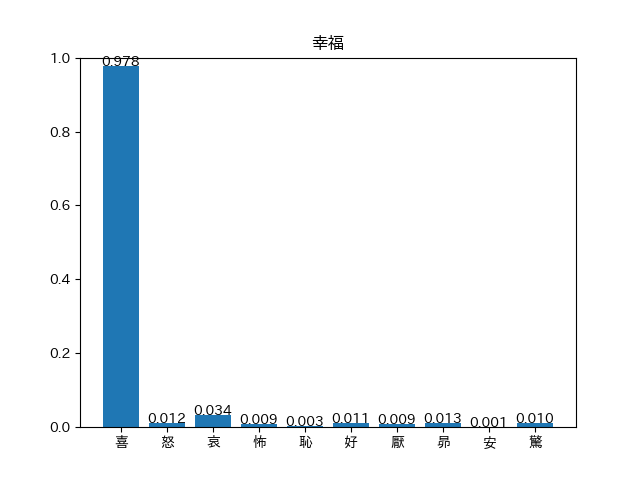
\includegraphics[keepaspectratio, scale=0.45]{./figure/BERT+weight/Q05/001.png}
			\subcaption{「幸福」に対する感情ベクトル}
		\end{minipage} &
		\begin{minipage}[t]{0.45\hsize}
			\centering
			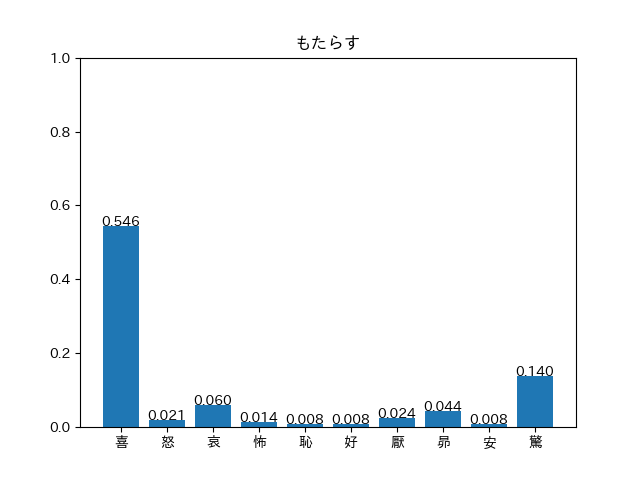
\includegraphics[keepaspectratio, scale=0.45]{./figure/BERT+weight/Q05/002.png}
			\subcaption{「もたらす」に対する感情ベクトル}
		\end{minipage} \\
		\begin{minipage}[t]{0.45\hsize}
			\centering
			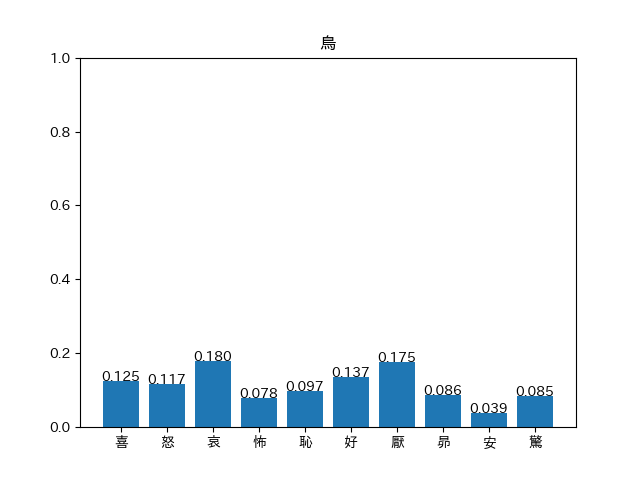
\includegraphics[keepaspectratio, scale=0.45]{./figure/BERT+weight/Q05/003.png}
			\subcaption{「鳥」に対する感情ベクトル}
		\end{minipage} \\
	\end{tabular}
	\caption{「幸福をもたらす鳥.」に対する各単語の感情ベクトル}
	\label{fig:output_q05}
\end{figure}

\begin{figure}[H]
	\begin{tabular}{cc}
		\begin{minipage}[t]{0.45\hsize}
			\centering
			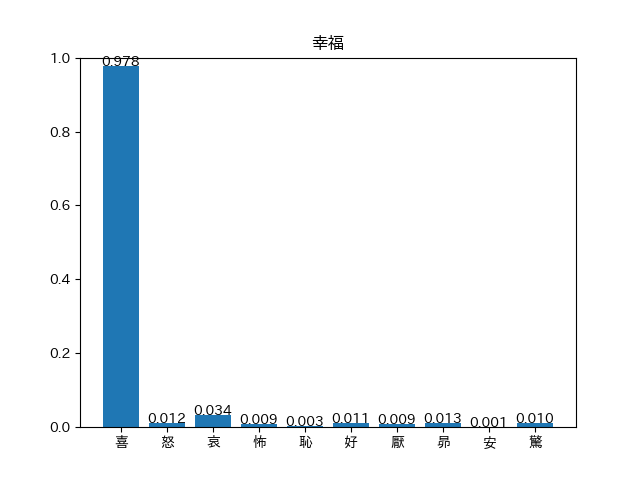
\includegraphics[keepaspectratio, scale=0.45]{./figure/BERT+weight/Q05/001.png}
			\subcaption{「不運」に対する感情ベクトル}
		\end{minipage} &
		\begin{minipage}[t]{0.45\hsize}
			\centering
			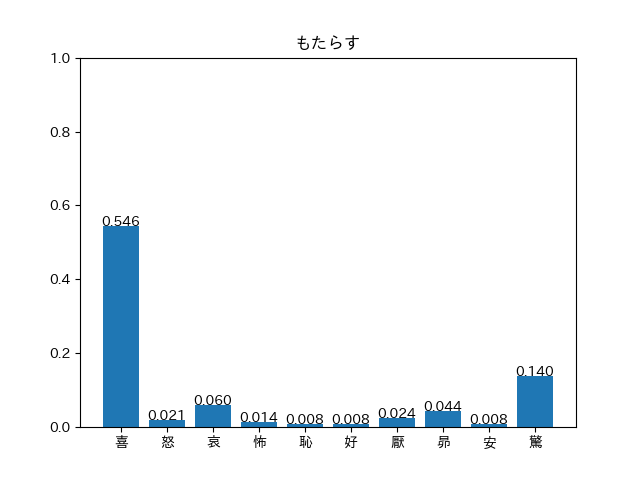
\includegraphics[keepaspectratio, scale=0.45]{./figure/BERT+weight/Q05/002.png}
			\subcaption{「もたらす」に対する感情ベクトル}
		\end{minipage} \\
		\begin{minipage}[t]{0.45\hsize}
			\centering
			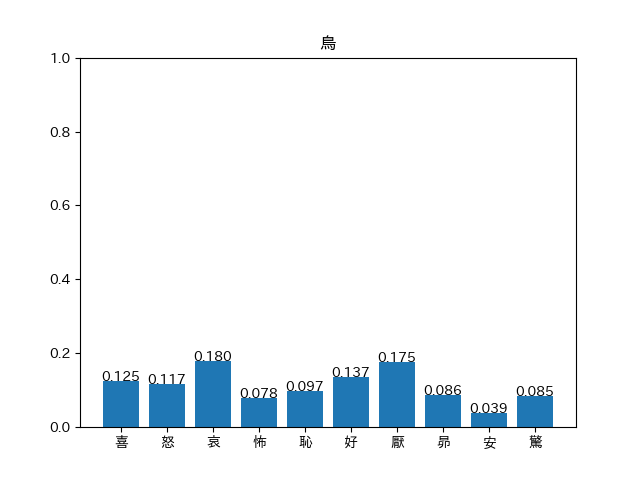
\includegraphics[keepaspectratio, scale=0.45]{./figure/BERT+weight/Q05/003.png}
			\subcaption{「行い」に対する感情ベクトル}
		\end{minipage} \\
	\end{tabular}
	\caption{「不運をもたらす行い.」に対する各単語の感情ベクトル}
	\label{fig:output_q06}
\end{figure}

\begin{figure}[H]
	\begin{tabular}{cc}
		\begin{minipage}[t]{0.45\hsize}
			\centering
			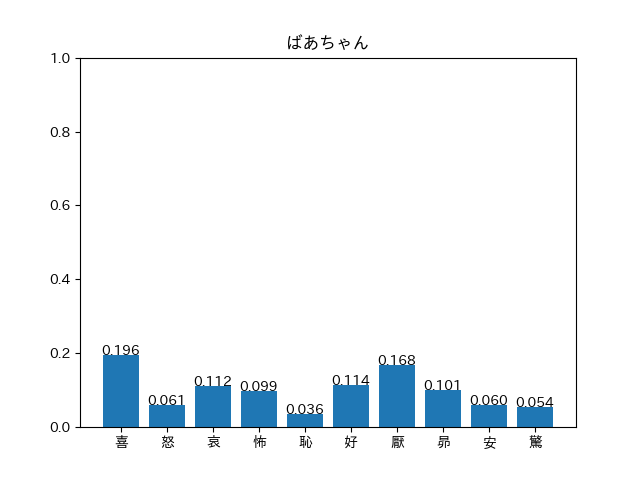
\includegraphics[keepaspectratio, scale=0.45]{./figure/BERT+weight/Q11/001.png}
			\subcaption{「ばあちゃん」に対する感情ベクトル}
		\end{minipage} &
		\begin{minipage}[t]{0.45\hsize}
			\centering
			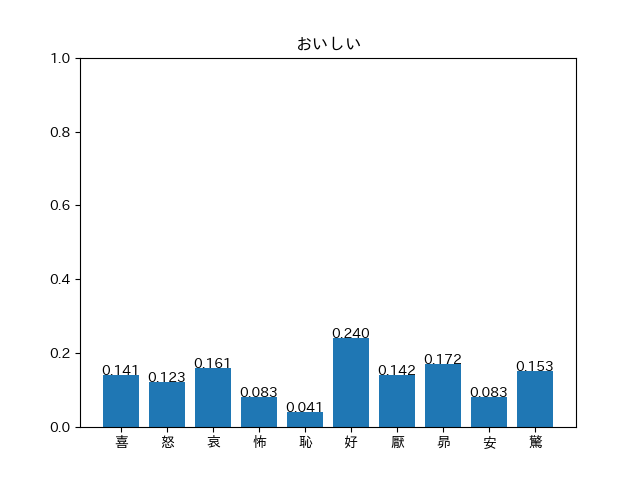
\includegraphics[keepaspectratio, scale=0.45]{./figure/BERT+weight/Q11/002.png}
			\subcaption{「おいしい」に対する感情ベクトル}
		\end{minipage} \\
		\begin{minipage}[t]{0.45\hsize}
			\centering
			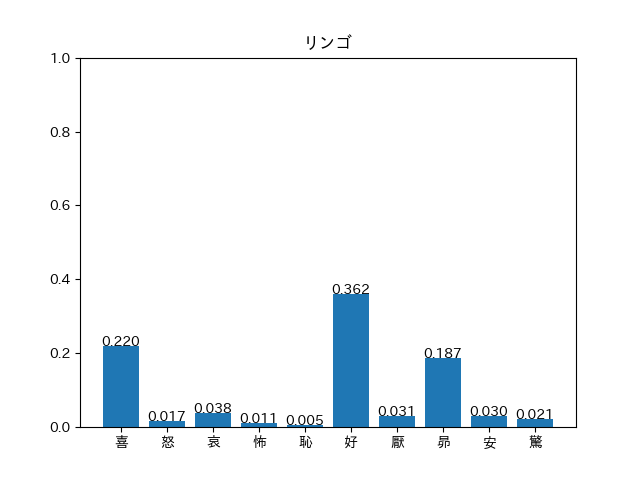
\includegraphics[keepaspectratio, scale=0.45]{./figure/BERT+weight/Q11/003.png}
			\subcaption{「リンゴ」に対する感情ベクトル}
		\end{minipage} &
		\begin{minipage}[t]{0.45\hsize}
			\centering
			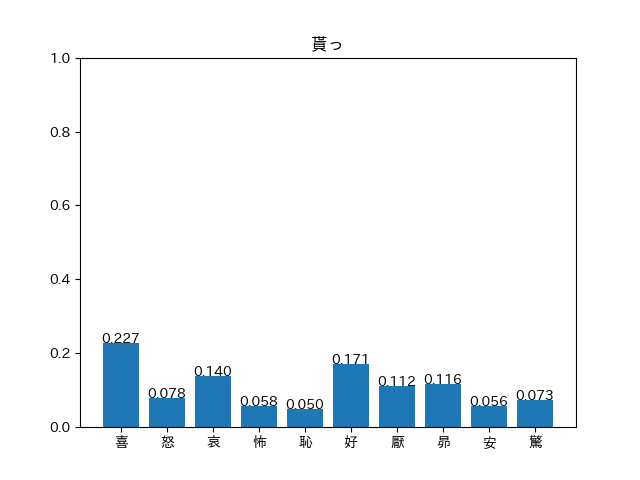
\includegraphics[keepaspectratio, scale=0.45]{./figure/BERT+weight/Q11/004.png}
			\subcaption{「貰っ」に対する感情ベクトル}
		\end{minipage} \\
	\end{tabular}
	\caption{「おばあちゃんからおいしいリンゴを貰った.」に対する各単語の感情ベクトル}
	\label{fig:output_q11}
\end{figure}

\begin{figure}[H]
	\begin{tabular}{cc}
		\begin{minipage}[t]{0.45\hsize}
			\centering
			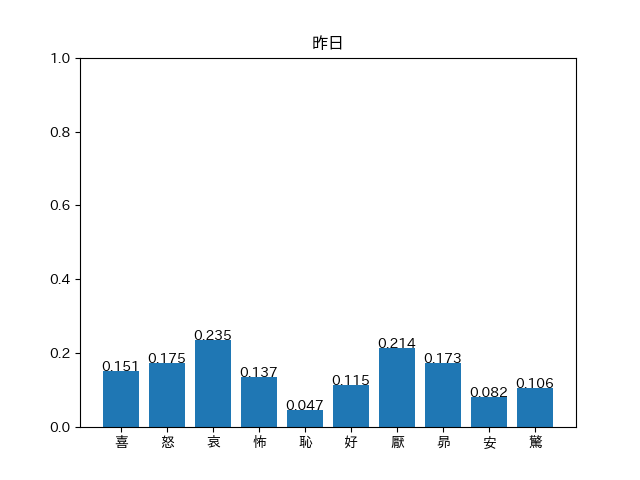
\includegraphics[keepaspectratio, scale=0.45]{./figure/BERT+weight/Q12/001.png}
			\subcaption{「昨日」に対する感情ベクトル}
		\end{minipage} &
		\begin{minipage}[t]{0.45\hsize}
			\centering
			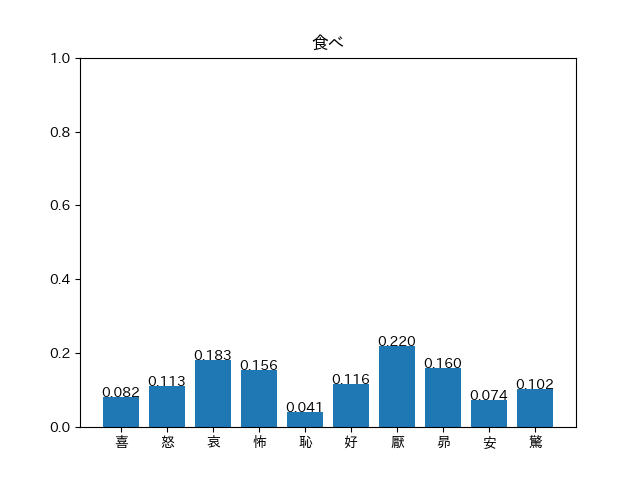
\includegraphics[keepaspectratio, scale=0.45]{./figure/BERT+weight/Q12/002.png}
			\subcaption{「食べ」に対する感情ベクトル}
		\end{minipage} \\
		\begin{minipage}[t]{0.45\hsize}
			\centering
			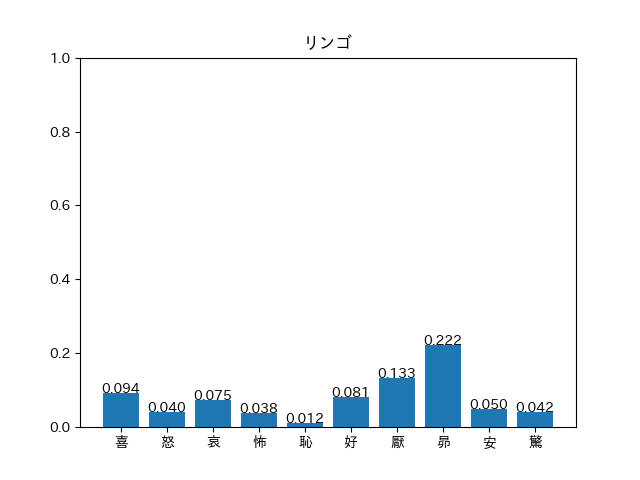
\includegraphics[keepaspectratio, scale=0.45]{./figure/BERT+weight/Q12/003.png}
			\subcaption{「リンゴ」に対する感情ベクトル}
		\end{minipage} &
		\begin{minipage}[t]{0.45\hsize}
			\centering
			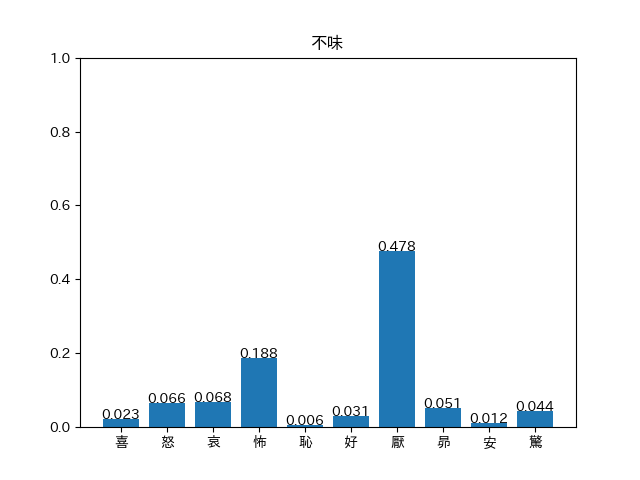
\includegraphics[keepaspectratio, scale=0.45]{./figure/BERT+weight/Q12/004.png}
			\subcaption{「不味」に対する感情ベクトル}
		\end{minipage} \\
	\end{tabular}
	\caption{「昨日食べたリンゴが不味すぎた.」に対する各単語の感情ベクトル}
	\label{fig:output_q12}
\end{figure}

\begin{figure}[H]
	\begin{tabular}{cc}
		\begin{minipage}[t]{0.45\hsize}
			\centering
			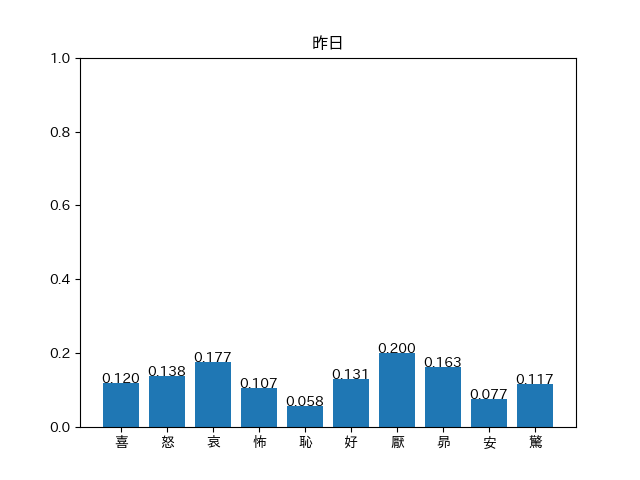
\includegraphics[keepaspectratio, scale=0.45]{./figure/BERT+weight/Q23/001.png}
			\subcaption{「昨日」に対する感情ベクトル}
		\end{minipage} &
		\begin{minipage}[t]{0.45\hsize}
			\centering
			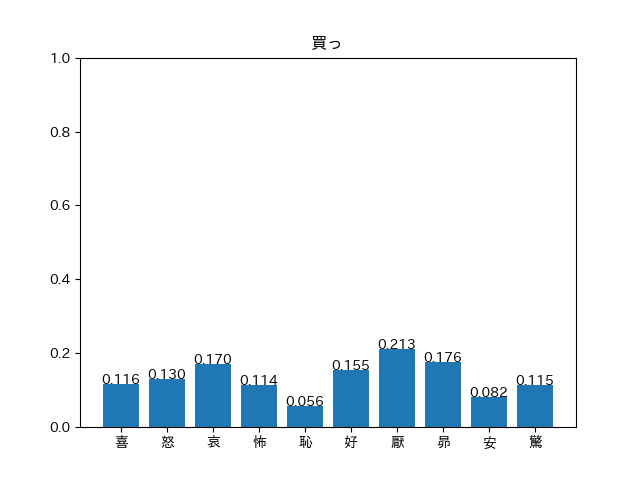
\includegraphics[keepaspectratio, scale=0.45]{./figure/BERT+weight/Q23/002.png}
			\subcaption{「買っ」に対する感情ベクトル}
		\end{minipage} \\
		\begin{minipage}[t]{0.45\hsize}
			\centering
			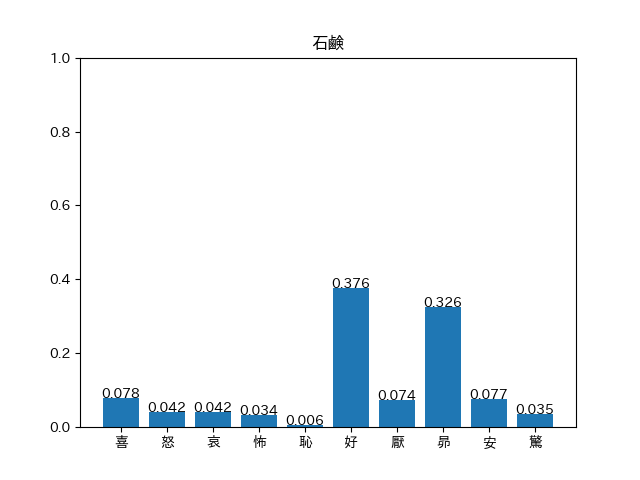
\includegraphics[keepaspectratio, scale=0.45]{./figure/BERT+weight/Q23/003.png}
			\subcaption{「石鹸」に対する感情ベクトル}
		\end{minipage} &
		\begin{minipage}[t]{0.45\hsize}
			\centering
			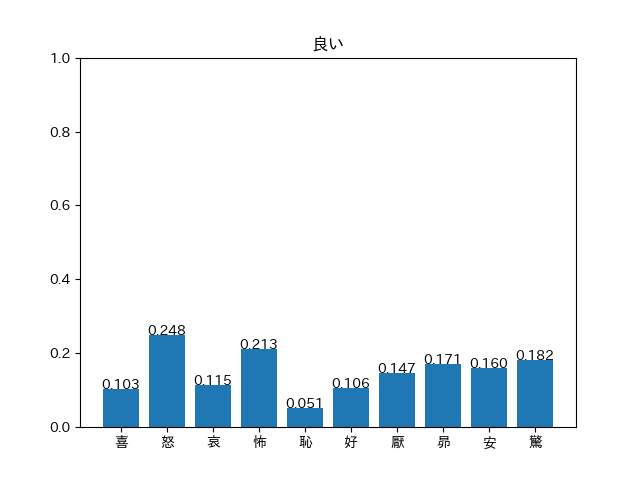
\includegraphics[keepaspectratio, scale=0.45]{./figure/BERT+weight/Q23/004.png}
			\subcaption{「良い」に対する感情ベクトル}
		\end{minipage} \\
		\begin{minipage}[t]{0.45\hsize}
			\centering
			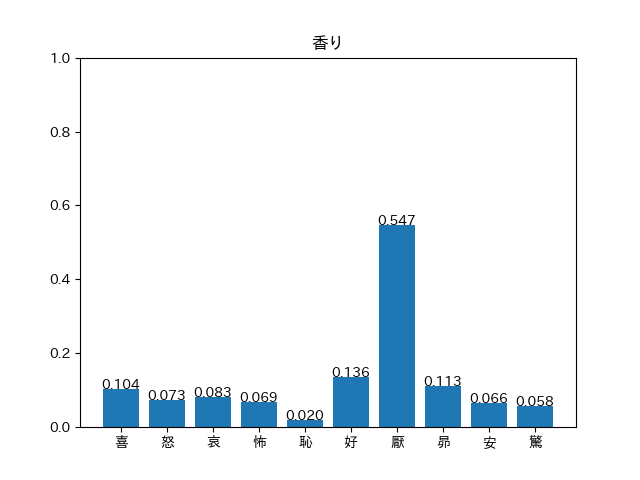
\includegraphics[keepaspectratio, scale=0.45]{./figure/BERT+weight/Q23/005.png}
			\subcaption{「香り」に対する感情ベクトル}
		\end{minipage} \\
	\end{tabular}
	\caption{「昨日買った石鹸は良い香りがする.」に対する各単語の感情ベクトル}
	\label{fig:output_q23}
\end{figure}

\begin{figure}[H]
	\begin{tabular}{cc}
		\begin{minipage}[t]{0.45\hsize}
			\centering
			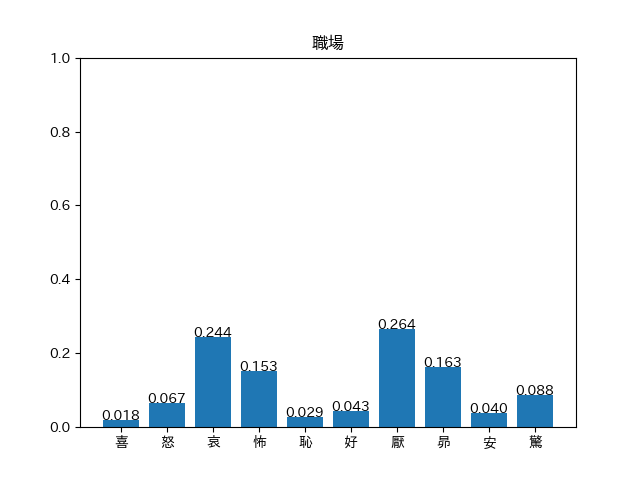
\includegraphics[keepaspectratio, scale=0.45]{./figure/BERT+weight/Q24/001.png}
			\subcaption{「職場」に対する感情ベクトル}
		\end{minipage} &
		\begin{minipage}[t]{0.45\hsize}
			\centering
			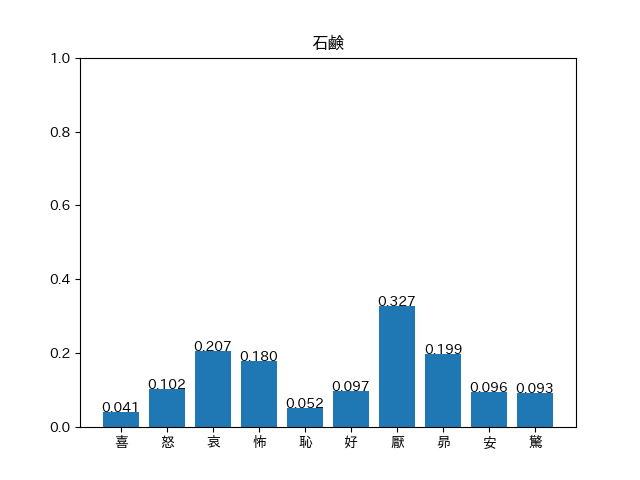
\includegraphics[keepaspectratio, scale=0.45]{./figure/BERT+weight/Q24/002.png}
			\subcaption{「石鹸」に対する感情ベクトル}
		\end{minipage} \\
		\begin{minipage}[t]{0.45\hsize}
			\centering
			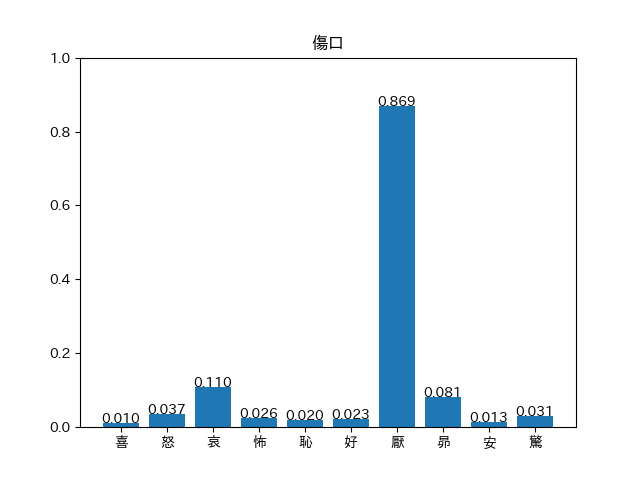
\includegraphics[keepaspectratio, scale=0.45]{./figure/BERT+weight/Q24/003.png}
			\subcaption{「傷口」に対する感情ベクトル}
		\end{minipage} \\
	\end{tabular}
	\caption{「職場の石鹸は傷口に沁みる.」に対する各単語の感情ベクトル}
	\label{fig:output_q24}
\end{figure}

\begin{figure}[H]
	\begin{tabular}{cc}
		\begin{minipage}[t]{0.45\hsize}
			\centering
			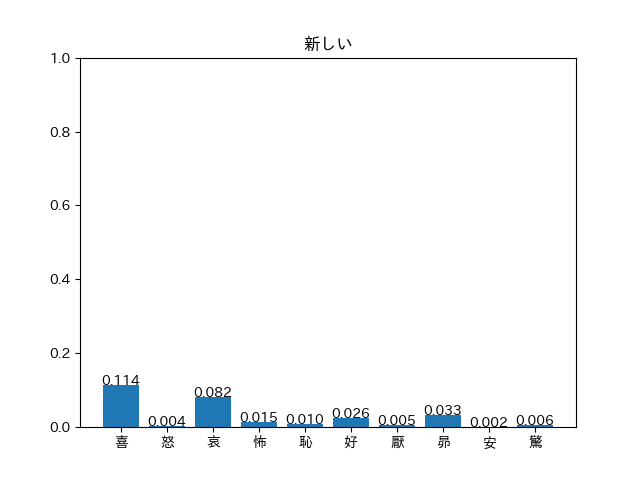
\includegraphics[keepaspectratio, scale=0.45]{./figure/BERT+weight/Q29/001.png}
			\subcaption{「新しい」に対する感情ベクトル}
		\end{minipage} &
		\begin{minipage}[t]{0.45\hsize}
			\centering
			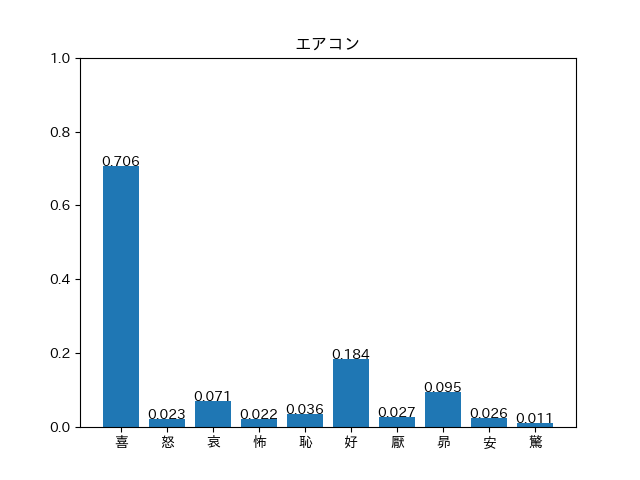
\includegraphics[keepaspectratio, scale=0.45]{./figure/BERT+weight/Q29/002.png}
			\subcaption{「エアコン」に対する感情ベクトル}
		\end{minipage} \\
		\begin{minipage}[t]{0.45\hsize}
			\centering
			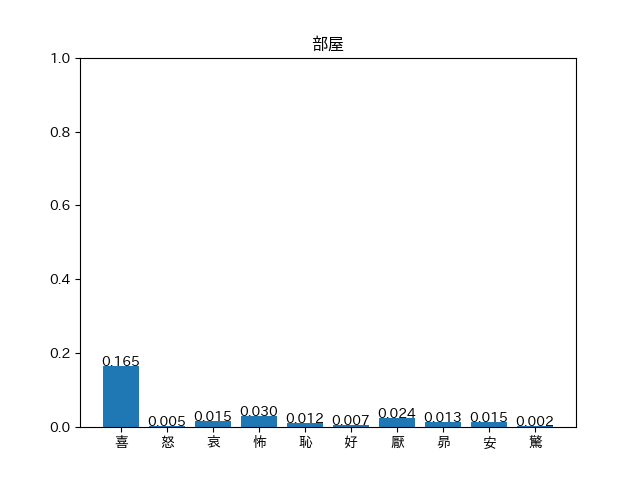
\includegraphics[keepaspectratio, scale=0.45]{./figure/BERT+weight/Q29/003.png}
			\subcaption{「部屋」に対する感情ベクトル}
		\end{minipage} &
		\begin{minipage}[t]{0.45\hsize}
			\centering
			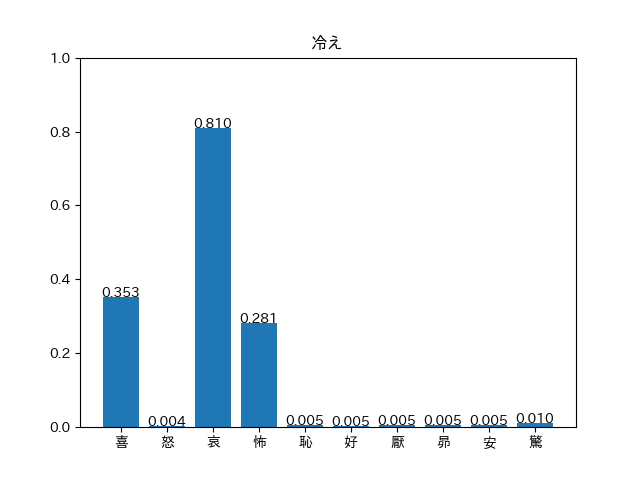
\includegraphics[keepaspectratio, scale=0.45]{./figure/BERT+weight/Q29/004.png}
			\subcaption{「冷え」に対する感情ベクトル}
		\end{minipage} \\
		\begin{minipage}[t]{0.45\hsize}
			\centering
			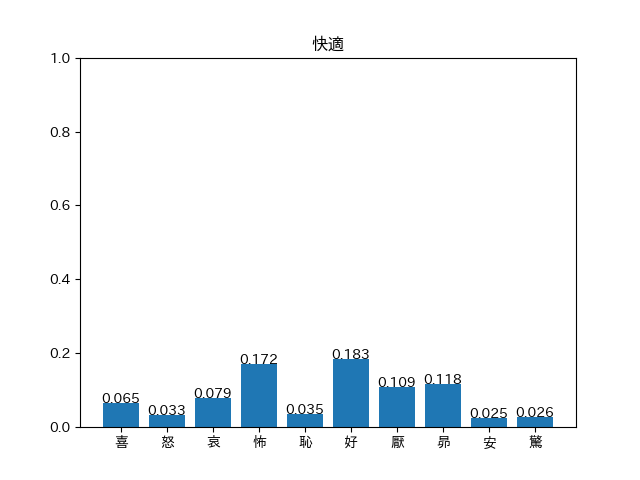
\includegraphics[keepaspectratio, scale=0.45]{./figure/BERT+weight/Q29/005.png}
			\subcaption{「快適」に対する感情ベクトル}
		\end{minipage} \\
	\end{tabular}
	\caption{「新しいエアコンは、部屋がよく冷えてとても快適である.」に対する各単語の感情ベクトル}
	\label{fig:output_q29}
\end{figure}

\begin{figure}[H]
	\begin{tabular}{cc}
		\begin{minipage}[t]{0.45\hsize}
			\centering
			\includegraphics[keepaspectratio, scale=0.45]{./figure/BERT+weight/Q30/001.png}
			\subcaption{「リビング」に対する感情ベクトル}
		\end{minipage} &
		\begin{minipage}[t]{0.45\hsize}
			\centering
			\includegraphics[keepaspectratio, scale=0.45]{./figure/BERT+weight/Q30/002.png}
			\subcaption{「エアコン」に対する感情ベクトル}
		\end{minipage} \\
		\begin{minipage}[t]{0.45\hsize}
			\centering
			\includegraphics[keepaspectratio, scale=0.45]{./figure/BERT+weight/Q30/003.png}
			\subcaption{「故障」に対する感情ベクトル}
		\end{minipage} &
		\begin{minipage}[t]{0.45\hsize}
			\centering
			\includegraphics[keepaspectratio, scale=0.45]{./figure/BERT+weight/Q30/004.png}
			\subcaption{「しまっ」に対する感情ベクトル}
		\end{minipage} \\
	\end{tabular}
	\caption{「リビングのエアコンが故障してしまった.」に対する各単語の感情ベクトル}
	\label{fig:output_q30}
\end{figure}

\begin{figure}[H]
	\begin{tabular}{cc}
		\begin{minipage}[t]{0.45\hsize}
			\centering
			\includegraphics[keepaspectratio, scale=0.45]{./figure/BERT+weight/Q72/001.png}
			\subcaption{「笑み」に対する感情ベクトル}
		\end{minipage} &
		\begin{minipage}[t]{0.45\hsize}
			\centering
			\includegraphics[keepaspectratio, scale=0.45]{./figure/BERT+weight/Q72/002.png}
			\subcaption{「浮かべ」に対する感情ベクトル}
		\end{minipage} \\
	\end{tabular}
	\caption{「彼は笑みを浮かべた.」に対する各単語の感情ベクトル}
	\label{fig:output_q72}
\end{figure}

\begin{figure}[H]
	\begin{tabular}{cc}
		\begin{minipage}[t]{0.45\hsize}
			\centering
			\includegraphics[keepaspectratio, scale=0.45]{./figure/BERT+weight/Q74/001.png}
			\subcaption{「寒く」に対する感情ベクトル}
		\end{minipage} &
		\begin{minipage}[t]{0.45\hsize}
			\centering
			\includegraphics[keepaspectratio, scale=0.45]{./figure/BERT+weight/Q74/002.png}
			\subcaption{「くる」に対する感情ベクトル}
		\end{minipage} \\
		\begin{minipage}[t]{0.45\hsize}
			\centering
			\includegraphics[keepaspectratio, scale=0.45]{./figure/BERT+weight/Q74/003.png}
			\subcaption{「こたつ」に対する感情ベクトル}
		\end{minipage} &
		\begin{minipage}[t]{0.45\hsize}
			\centering
			\includegraphics[keepaspectratio, scale=0.45]{./figure/BERT+weight/Q74/004.png}
			\subcaption{「恋しい」に対する感情ベクトル}
		\end{minipage} \\
	\end{tabular}
	\caption{「寒くなってくると、こたつが恋しい.」に対する各単語の感情ベクトル}
	\label{fig:output_q74}
\end{figure}

\begin{figure}[H]
	\begin{tabular}{cc}
		\begin{minipage}[t]{0.45\hsize}
			\centering
			\includegraphics[keepaspectratio, scale=0.45]{./figure/BERT+weight/Q80/001.png}
			\subcaption{「愚か」に対する感情ベクトル}
		\end{minipage} &
		\begin{minipage}[t]{0.45\hsize}
			\centering
			\includegraphics[keepaspectratio, scale=0.45]{./figure/BERT+weight/Q80/002.png}
			\subcaption{「行動」に対する感情ベクトル}
		\end{minipage} \\
		\begin{minipage}[t]{0.45\hsize}
			\centering
			\includegraphics[keepaspectratio, scale=0.45]{./figure/BERT+weight/Q80/003.png}
			\subcaption{「立腹」に対する感情ベクトル}
		\end{minipage} \\
	\end{tabular}
	\caption{「愚かな行動に立腹した.」に対する各単語の感情ベクトル}
	\label{fig:output_q80}
\end{figure}

\begin{figure}[H]
	\begin{tabular}{cc}
		\begin{minipage}[t]{0.45\hsize}
			\centering
			\includegraphics[keepaspectratio, scale=0.45]{./figure/BERT+weight/Q85/001.png}
			\subcaption{「因縁」に対する感情ベクトル}
		\end{minipage} &
		\begin{minipage}[t]{0.45\hsize}
			\centering
			\includegraphics[keepaspectratio, scale=0.45]{./figure/BERT+weight/Q85/002.png}
			\subcaption{「ライバル」に対する感情ベクトル}
		\end{minipage} \\
		\begin{minipage}[t]{0.45\hsize}
			\centering
			\includegraphics[keepaspectratio, scale=0.45]{./figure/BERT+weight/Q85/003.png}
			\subcaption{「倒す」に対する感情ベクトル}
		\end{minipage} &
		\begin{minipage}[t]{0.45\hsize}
			\centering
			\includegraphics[keepaspectratio, scale=0.45]{./figure/BERT+weight/Q85/004.png}
			\subcaption{「嬉し涙」に対する感情ベクトル}
		\end{minipage} \\
		\begin{minipage}[t]{0.45\hsize}
			\centering
			\includegraphics[keepaspectratio, scale=0.45]{./figure/BERT+weight/Q85/005.png}
			\subcaption{「流し」に対する感情ベクトル}
		\end{minipage} \\
	\end{tabular}
	\caption{「因縁のライバルを倒すことができ、嬉し涙を流した.」に対する各単語の感情ベクトル}
	\label{fig:output_q85}
\end{figure}

\begin{figure}[H]
	\begin{tabular}{cc}
		\begin{minipage}[t]{0.45\hsize}
			\centering
			\includegraphics[keepaspectratio, scale=0.45]{./figure/BERT+weight/Q39/001.png}
			\subcaption{「話す」に対する感情ベクトル}
		\end{minipage} &
		\begin{minipage}[t]{0.45\hsize}
			\centering
			\includegraphics[keepaspectratio, scale=0.45]{./figure/BERT+weight/Q39/002.png}
			\subcaption{「楽しい」に対する感情ベクトル}
		\end{minipage} \\
		\begin{minipage}[t]{0.45\hsize}
			\centering
			\includegraphics[keepaspectratio, scale=0.45]{./figure/BERT+weight/Q39/003.png}
			\subcaption{「気持ち」に対する感情ベクトル}
		\end{minipage} \\
	\end{tabular}
	\caption{「彼女と話すと楽しい気持ちになる.」に対する各単語の感情ベクトル}
	\label{fig:output_q39}
\end{figure}

\begin{figure}[H]
	\begin{tabular}{cc}
		\begin{minipage}[t]{0.45\hsize}
			\centering
			\includegraphics[keepaspectratio, scale=0.45]{./figure/BERT+weight/Q43/001.png}
			\subcaption{「目」に対する感情ベクトル}
		\end{minipage} &
		\begin{minipage}[t]{0.45\hsize}
			\centering
			\includegraphics[keepaspectratio, scale=0.45]{./figure/BERT+weight/Q43/002.png}
			\subcaption{「前」に対する感情ベクトル}
		\end{minipage} \\
		\begin{minipage}[t]{0.45\hsize}
			\centering
			\includegraphics[keepaspectratio, scale=0.45]{./figure/BERT+weight/Q43/003.png}
			\subcaption{「事故」に対する感情ベクトル}
		\end{minipage} &
		\begin{minipage}[t]{0.45\hsize}
			\centering
			\includegraphics[keepaspectratio, scale=0.45]{./figure/BERT+weight/Q43/004.png}
			\subcaption{「見」に対する感情ベクトル}
		\end{minipage} \\
		\begin{minipage}[t]{0.45\hsize}
			\centering
			\includegraphics[keepaspectratio, scale=0.45]{./figure/BERT+weight/Q43/005.png}
			\subcaption{「悲しい」に対する感情ベクトル}
		\end{minipage} &
		\begin{minipage}[t]{0.45\hsize}
			\centering
			\includegraphics[keepaspectratio, scale=0.45]{./figure/BERT+weight/Q43/006.png}
			\subcaption{「気持ち」に対する感情ベクトル}
		\end{minipage} \\
	\end{tabular}
	\caption{「目の前で大きな事故を見てしまい、悲しい気持ちになった.」に対する各単語の感情ベクトル}
	\label{fig:output_q43}
\end{figure}


\begin{figure}[H]
	\begin{tabular}{cc}
		\begin{minipage}[t]{0.45\hsize}
			\centering
			\includegraphics[keepaspectratio, scale=0.45]{./figure/BERT+weight/Q51/001.png}
			\subcaption{「久々」に対する感情ベクトル}
		\end{minipage} &
		\begin{minipage}[t]{0.45\hsize}
			\centering
			\includegraphics[keepaspectratio, scale=0.45]{./figure/BERT+weight/Q51/002.png}
			\subcaption{「再会」に対する感情ベクトル}
		\end{minipage} \\
		\begin{minipage}[t]{0.45\hsize}
			\centering
			\includegraphics[keepaspectratio, scale=0.45]{./figure/BERT+weight/Q51/003.png}
			\subcaption{「涙」に対する感情ベクトル}
		\end{minipage} &
		\begin{minipage}[t]{0.45\hsize}
			\centering
			\includegraphics[keepaspectratio, scale=0.45]{./figure/BERT+weight/Q51/004.png}
			\subcaption{「流し」に対する感情ベクトル}
		\end{minipage} \\
		\begin{minipage}[t]{0.45\hsize}
			\centering
			\includegraphics[keepaspectratio, scale=0.45]{./figure/BERT+weight/Q51/005.png}
			\subcaption{「喜ん」に対する感情ベクトル}
		\end{minipage} \\
	\end{tabular}
	\caption{「久々の再会に涙を流して喜んだ.」に対する各単語の感情ベクトル}
	\label{fig:output_q51}
\end{figure}

\begin{figure}[H]
	\begin{tabular}{cc}
		\begin{minipage}[t]{0.45\hsize}
			\centering
			\includegraphics[keepaspectratio, scale=0.45]{./figure/BERT+weight/Q55/001.png}
			\subcaption{「紛争」に対する感情ベクトル}
		\end{minipage} &
		\begin{minipage}[t]{0.45\hsize}
			\centering
			\includegraphics[keepaspectratio, scale=0.45]{./figure/BERT+weight/Q55/002.png}
			\subcaption{「悲惨」に対する感情ベクトル}
		\end{minipage} \\
		\begin{minipage}[t]{0.45\hsize}
			\centering
			\includegraphics[keepaspectratio, scale=0.45]{./figure/BERT+weight/Q55/003.png}
			\subcaption{「実態」に対する感情ベクトル}
		\end{minipage} &
		\begin{minipage}[t]{0.45\hsize}
			\centering
			\includegraphics[keepaspectratio, scale=0.45]{./figure/BERT+weight/Q55/004.png}
			\subcaption{「知り」に対する感情ベクトル}
		\end{minipage} \\
		\begin{minipage}[t]{0.45\hsize}
			\centering
			\includegraphics[keepaspectratio, scale=0.45]{./figure/BERT+weight/Q55/005.png}
			\subcaption{「涙」に対する感情ベクトル}
		\end{minipage} &
		\begin{minipage}[t]{0.45\hsize}
			\centering
			\includegraphics[keepaspectratio, scale=0.45]{./figure/BERT+weight/Q55/006.png}
			\subcaption{「止まら」に対する感情ベクトル}
		\end{minipage} \\
	\end{tabular}
	\caption{「紛争の悲惨な実態を知り、涙が止まらない.」に対する各単語の感情ベクトル}
	\label{fig:output_q55}
\end{figure}

\begin{figure}[H]
	\begin{tabular}{cc}
		\begin{minipage}[t]{0.45\hsize}
			\centering
			\includegraphics[keepaspectratio, scale=0.45]{./figure/BERT+weight/Q62/001.png}
			\subcaption{「世界一」に対する感情ベクトル}
		\end{minipage} &
		\begin{minipage}[t]{0.45\hsize}
			\centering
			\includegraphics[keepaspectratio, scale=0.45]{./figure/BERT+weight/Q62/002.png}
			\subcaption{「選手」に対する感情ベクトル}
		\end{minipage} \\
		\begin{minipage}[t]{0.45\hsize}
			\centering
			\includegraphics[keepaspectratio, scale=0.45]{./figure/BERT+weight/Q62/003.png}
			\subcaption{「たい」に対する感情ベクトル}
		\end{minipage} &
		\begin{minipage}[t]{0.45\hsize}
			\centering
			\includegraphics[keepaspectratio, scale=0.45]{./figure/BERT+weight/Q62/004.png}
			\subcaption{「思い」に対する感情ベクトル}
		\end{minipage} \\
		\begin{minipage}[t]{0.45\hsize}
			\centering
			\includegraphics[keepaspectratio, scale=0.45]{./figure/BERT+weight/Q62/005.png}
			\subcaption{「持っ」に対する感情ベクトル}
		\end{minipage} \\
	\end{tabular}
	\caption{「彼は世界一の選手になりたいという思いを持っている.」に対する各単語の感情ベクトル}
	\label{fig:output_q62}
\end{figure}

\begin{figure}[H]
	\begin{tabular}{cc}
		\begin{minipage}[t]{0.45\hsize}
			\centering
			\includegraphics[keepaspectratio, scale=0.45]{./figure/BERT+weight/Q69/001.png}
			\subcaption{「うまく」に対する感情ベクトル}
		\end{minipage} &
		\begin{minipage}[t]{0.45\hsize}
			\centering
			\includegraphics[keepaspectratio, scale=0.45]{./figure/BERT+weight/Q69/002.png}
			\subcaption{「多く」に対する感情ベクトル}
		\end{minipage} \\
		\begin{minipage}[t]{0.45\hsize}
			\centering
			\includegraphics[keepaspectratio, scale=0.45]{./figure/BERT+weight/Q69/003.png}
			\subcaption{「つらい」に対する感情ベクトル}
		\end{minipage} &
		\begin{minipage}[t]{0.45\hsize}
			\centering
			\includegraphics[keepaspectratio, scale=0.45]{./figure/BERT+weight/Q69/004.png}
			\subcaption{「思い」に対する感情ベクトル}
		\end{minipage} \\
		\begin{minipage}[t]{0.45\hsize}
			\centering
			\includegraphics[keepaspectratio, scale=0.45]{./figure/BERT+weight/Q69/005.png}
			\subcaption{「抱え」に対する感情ベクトル}
		\end{minipage} \\
	\end{tabular}
	\caption{「うまくいかないことが多く、つらい思いを抱えている.」に対する各単語の感情ベクトル}
	\label{fig:output_q69}
\end{figure}
\chapter{ニューラルネットワークの学習について}

\section{学習の様子}
	評価実験で用いたBERT+weight, BERT, embeddingの3手法について,
	それぞれのネットワーク学習時のふるまいを示す.
	以下の図\ref{fig:BERT_plus_weight_loss}~\ref{fig:embedding_loss}は,
	各モデルを学習しているときの
	train loss, validation lossの推移を示したグラフである.

	\begin{figure}[H]
		\centering
		\includegraphics[keepaspectratio, scale=0.8]{./figure/BERT+weight.png}
		\caption{BERT+weightの学習中の各種lossの推移}
		\label{fig:BERT_plus_weight_loss}
	\end{figure}

	\begin{figure}[H]
		\centering
		\includegraphics[keepaspectratio, scale=0.8]{./figure/BERT.png}
		\caption{BERTの学習中の各種lossの推移}
		\label{fig:BERT_loss}
	\end{figure}

	\begin{figure}[H]
		\centering
		\includegraphics[keepaspectratio, scale=0.8]{./figure/embeddings.png}
		\caption{embeddingの学習中の各種lossの推移}
		\label{fig:embedding_loss}
	\end{figure}

	なお,学習についてはEarly Stoppingを採用している.
	5回以上validation lossが更新されなかった場合に学習を停止し,
	それ以前でvalidation lossが最良であったネットワークを用いた.
	この時,各ネットワークの学習に要したエポック数と
	その時のtest lossは以下の表\ref{table:epoch_num}の通りである.

	\begin{table}[H]
		\centering
		\caption{各手法におけるネットワーク学習に要したエポック数とtest loss}
		\label{table:epoch_num}
		\begin{tabular}{|c|c|c|}
			\hline
			& エポック数 & test loss \\
			\hline
			BERT+weight & 23 & 0.0384 \\
			\hline
			BERT & 28 & 0.0792 \\
			\hline
			embedding & 15 & 0.1082 \\
			\hline
		\end{tabular}
	\end{table}

\section{ウィンドウサイズによる性能の変化}
	データセット生成時に感性語の周辺単語を収集する範囲である
	ウィンドウサイズを変化させたときの
	性能の変化について,BERT+weightとBERTのそれぞれで検証した.
	以下の表\ref{table:window_size}にその結果を示す.

	\begin{table}[H]
		\centering
		\caption{ウィンドウサイズの変化によるtest lossの変化}
		\label{table:window_size}
		\begin{tabular}{|c|c|c|c|}
			\hline
			& $W=2$ & $W=3$ & $W=4$ \\
			\hline
			BERT+weight & 0.0294 & 0.0384 & 0.0446 \\
			\hline
			BERT & 0.0670 & 0.0792 & 0.0863 \\
			\hline
		\end{tabular}
	\end{table}

	ウィンドウサイズが大きくなるほど学習完了時のlossが大きくなる傾向にある.
	これは,感情と直接的に関連しているわけではない一般単語の割合が高まり,
	感情推定の難易度が上がっていることが原因として考えられる.

	また,BERT+weightとBERTを比較すると,BERT+weightの方がlossの値が小さい傾向
	にある.
	これは,感性語ではない一般単語に対して強度を弱めた感情ベクトルを与えているためであり,
	システムが出力する値との誤差が小さくなることが原因であると考えられる.
	よって,test lossが小さいこととモデルの性能が高いことは
	必ずしも対応するとは限らないといえる.
\end{document}
